\documentclass{book}
\usepackage{amsmath, amsthm, amssymb, amsfonts}\usepackage{thmtools}\usepackage{parskip}\usepackage[pdftex]{graphicx}\usepackage[a4paper, margin=4cm]{geometry} % margins%
\usepackage{calc}\usepackage{setspace}\usepackage{geometry}\usepackage{float}\usepackage[hidelinks]{hyperref}\usepackage[utf8]{inputenc}\usepackage[english,danish]{babel}\usepackage{framed}\usepackage[dvipsnames,table]{xcolor} \usepackage{tcolorbox}\usepackage{hyperref}\usepackage{lastpage}\usepackage{fancyhdr}
%https://www.overleaf.com/learn/latex/Multiple_columns Linket her kan bruges til at indelle sider i kolumner
\usepackage{titlesec} %den her pakke bruges til at fjerne "Kapitel n" fra kapitelsidderne
\usepackage{minitoc}
\usepackage{gensymb} %Bruges til at kunne lave grader tegn
\usepackage{tcolorbox}
\usepackage{ifthen} % Skal bruges til sidebar
\usepackage{afterpage}
\renewcommand{\chaptermark}[1]{\markboth{#1}{}} % Fjerne kapitel nummeret fra headeren
\usepackage{tikz}
\titleformat{\chapter}[display] {\normalfont\huge\bfseries}{}{0pt}{\Huge} \pagestyle{fancy}
\fancyhf{} % Clear the header and footer
\fancyhead[LE,RO]{\thepage} % Page number on the outer (left on even, right on odd) side
\fancyhead[RE]{\leftmark} % Chapter title on the inner side (right on even pages)
\fancyhead[LO]{\leftmark} % Chapter title on the inner side (left on odd pages}
\definecolor{mahogany}{rgb}{192, 64, 0} % RGB for mahogany
\definecolor{gennemstegt}{rgb}{192, 112, 0}
\newcommand{\emptystar}{\textcolor{gray}{\textbf{$\star$}}}
\newcommand{\fullstar}{\textbf{$\star$}}

\title{Victors Kogebog med Stjålne Opskrifter}
\author{Victor Posselt Sandberg}
\date{Første udgave \quad \today}

\begin{document}
\dominitoc  

\frontmatter
\maketitle 
\begin{figure}
    \centering
    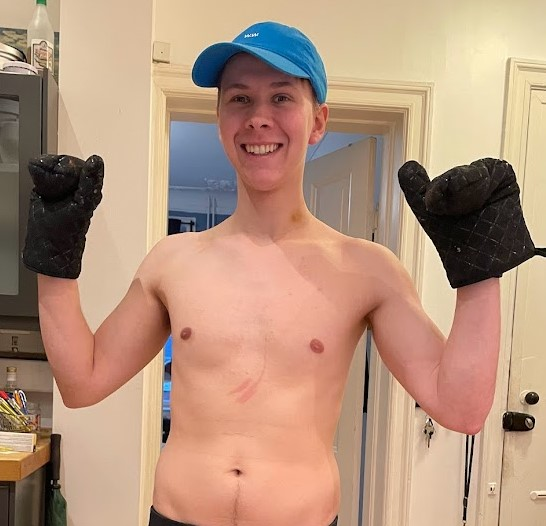
\includegraphics[width=1\linewidth]{Billeder/Mave2.jpg}
    \caption{Det er mig}
\end{figure}
\newpage \tableofcontents
\mainmatter
\newpage\chapter{Introduktion} 
Gennem de sidste 2 år har jeg haft til mål at lave mindst en ny opskrift per måned. Dette har bragt mig rundt omkring med unikke, spændende og lækre opskrifter. Jeg håber at denne bog kan få nogle inspirationer og nogle lækre måltider frem. 
\\Bogen er stadig et work in progress, da dette mål med en ny ret vil fortsætte. Udover dette, eksperimentere jeg også med hvilket setup, som giver bedst mening for en bog.
\\ Der er i særdeleshed lagt vægt på 2 afsnit, aftensmad og brød. Dette skyldes, at det især har været disse 2 felter jeg indtil videre har udforsket, den nuværende fordeling er subject to change, men indtil videre, alfabetisk opdeling inden for hvert kapitel, med vegetarisk og ikke-vegetarisk fordeling i aftensmaden. \\ Som udgangspunkt har jeg prøvet at undgå at bruge halve mål i mine opskrifter, da det giver en mere naturlig opdeling og mulighed for opskalering med hele tal. I de tilfælde hvor der er halve eller lignede, har jeg forsøgt at bruge brøker frem fra komma tal da jeg bruger "." som separator frem for "," til dagligt, og vil dermed prøve at undgå forvirring. \\ Bogen er eksporteret til PDF-format, med fungerende hyperlink, samt søge muligheder, da jeg vil fortsætte med at opdatere den er der her et link til den Drive mappe som jeg kommer til at ligge den op i: \\ 
\href{https://drive.google.com/drive/folders/1fln6GW-yU5_G8CKFQj_JbLBBnYhR5MEQ?usp=drive_link}{https://drive.google.com/drive/folders/1fln6GW-yU5\_G8CKFQj\_JbLBBnYhR5MEQ? \\ usp=drive\_link }
\\ Det er desværre ikke lige muligt at gøre det mere simpelt linket.
\\ \\ \textbf{Bon Appetit} 
\chapter{Morgenmad}
\minitoc
%\newpage \section{Bananpandekager}
\newpage \section{French Toast}
\begin{minipage}[t]{0.5\textwidth}
\textbf{Ingredienser:}
\begin{itemize}
    \item 1 Toastbrød (helst et i en fin størrelse, såsom multikernebrød fra Netto)
    \item 1 æg
    \item Eventuelt
    \begin{itemize}
        \item En skive ost
        \item Et stykke skinke
        \item Endnu et stykke toastbrød
        \item Forårsløg til pynt
    \end{itemize}
\end{itemize}
\end{minipage}
\begin{minipage}[t]{0.5\textwidth}
\textbf{Fremgangsmåde:}
\begin{enumerate}
    \item Skær et stykke af brødet ud fra midten, således ægget kan klæges deri.
    \item Steg på en pande, eventuelt med "låg".
    \item Hvis man vil have det som en parisertoast agtig, så læg ost, skinke og det andet stykke brød på.
    \item Lad brødet blive gylden brunt og vend
\end{enumerate}
\end{minipage}
\newpage \begin{tikzpicture}[remember picture,overlay,inner sep=0pt,outer sep=0pt]
    \node[anchor=south east] at (current page.south east) {
        \includegraphics[width=\paperwidth,height=\paperheight]{Billeder/Morgenmad/French_Toast3.jpg}
    };
\end{tikzpicture}
\clearpage \section{Røræg}
\begin{minipage}[t]{0.5\textwidth}
\textbf{Ingredienser:}
\begin{itemize}
\item  4 æg
\item 100 g cremefraiche eller græsk yoghurt
\item Salt, peber og evt. timian
\end{itemize}
\end{minipage}
\begin{minipage}[t]{0.5\textwidth}
 \textbf{Fremgangsmåde:}
\begin{enumerate}
    \item Bland æggene og mælkeproduktet sammen til en ensformig masse. 
    \item Steg på panden ved lav varme.\\
    OBS. Der kan med fordel vendes med en spisepind da det giver mindre smuldrende æg.
\end{enumerate}
\end{minipage}
\newpage \begin{tikzpicture}[remember picture,overlay,inner sep=0pt,outer sep=0pt]
    \node[anchor=south east] at (current page.south east) {
        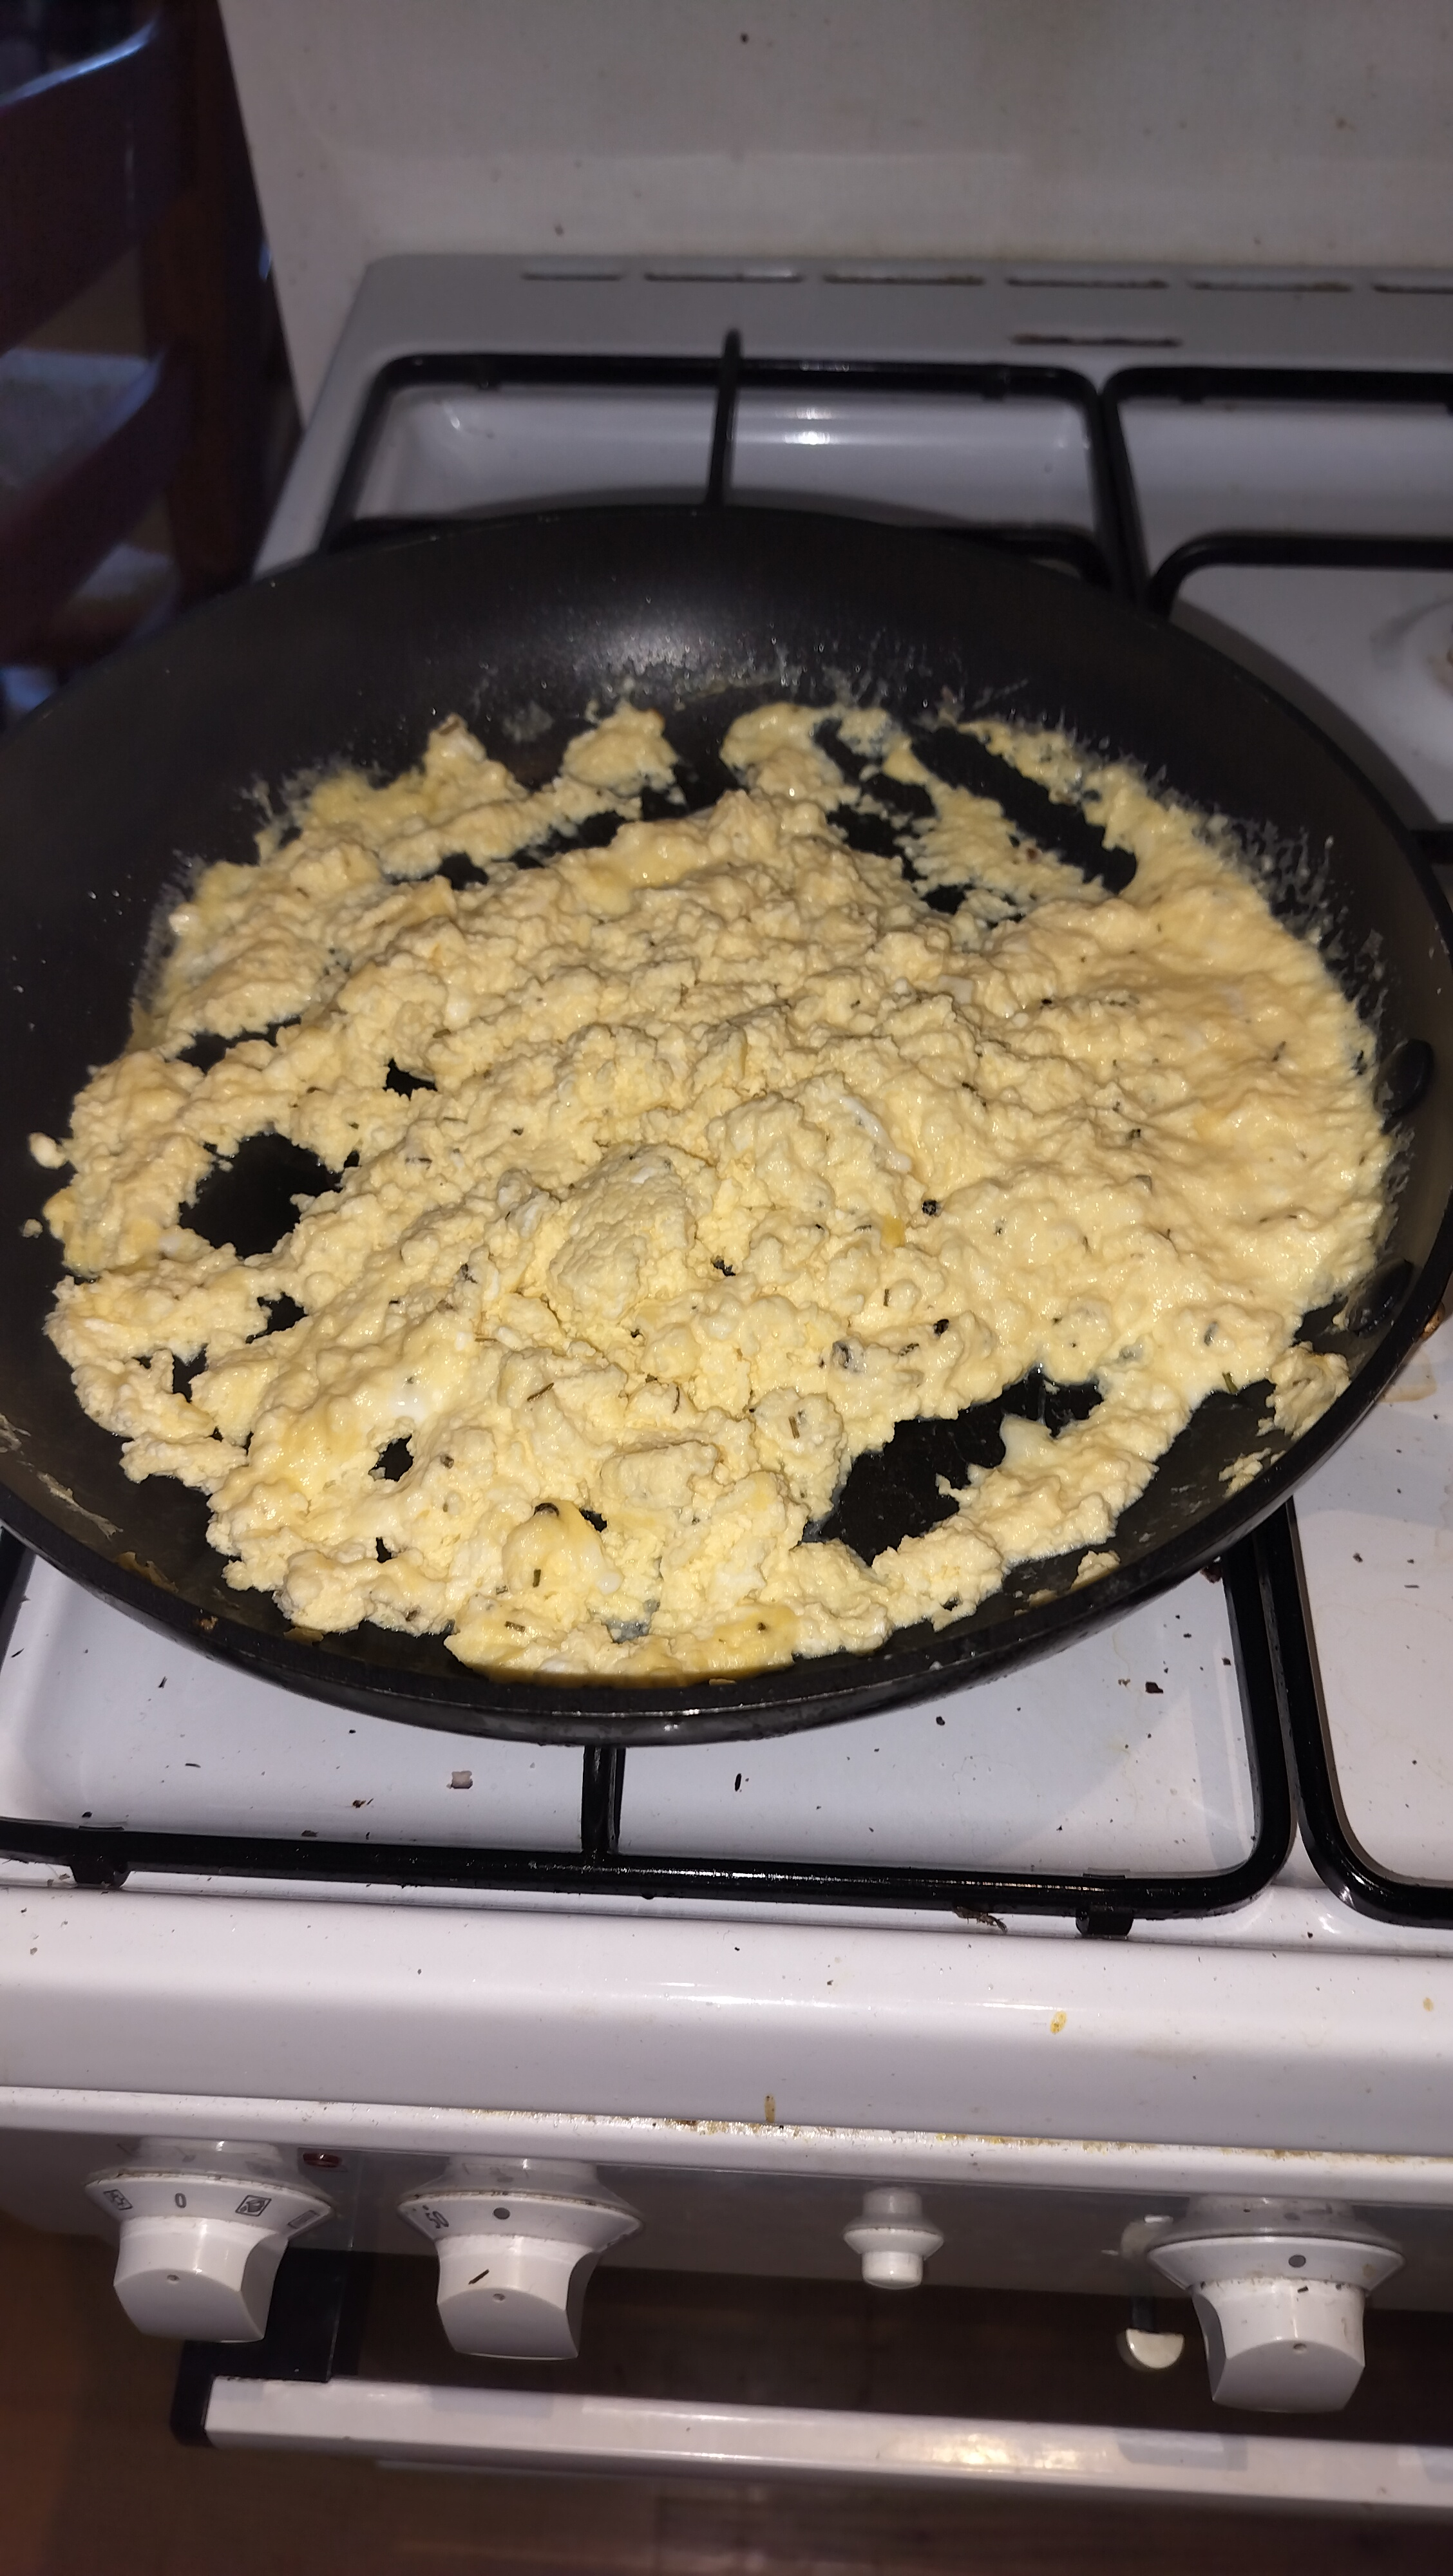
\includegraphics[width=\paperwidth,height=\paperheight]{Billeder/Morgenmad/Røræg.jpg}
    };
\end{tikzpicture}

\chapter{Frokost}
\minitoc
\clearpage \section{Couscous salat}
\begin{minipage}[t]{0.5\textwidth}
\textbf{Ingredienser:}
\begin{itemize}
    \item 200g Tørret couscous
    \item 500 mL kogende vand
    \item Krydderier
    \begin{itemize}
        \item Cayennepeber
        \item Paprika
    \end{itemize}
    \item Grøntsager
    \begin{itemize}
        \item Squash i tern
        \item Peberfrugt
        \item Aubergine
        \item Tomater
        \item Koriander
    \end{itemize}
\end{itemize}
\end{minipage}
\begin{minipage}[t]{0.5\textwidth}
\textbf{Fremgangsmåde:}
\begin{enumerate}
    \item Bland den tørrede couscous med de ønskede krydderier. 
    \item Held det kogende vand på couscoussen i en plastik skål og lad det trække. Der kan med fordel tilføjes mere vand, hvis man ønsker en mere "våd" salat.
    \item Tilsæt til sidst grøntsagerne og server eventuel med hummus.
\end{enumerate}
\end{minipage}
\newpage
\begin{tikzpicture}[remember picture,overlay,inner sep=0pt,outer sep=0pt]
    \node[anchor=south east] at (current page.south east) {
        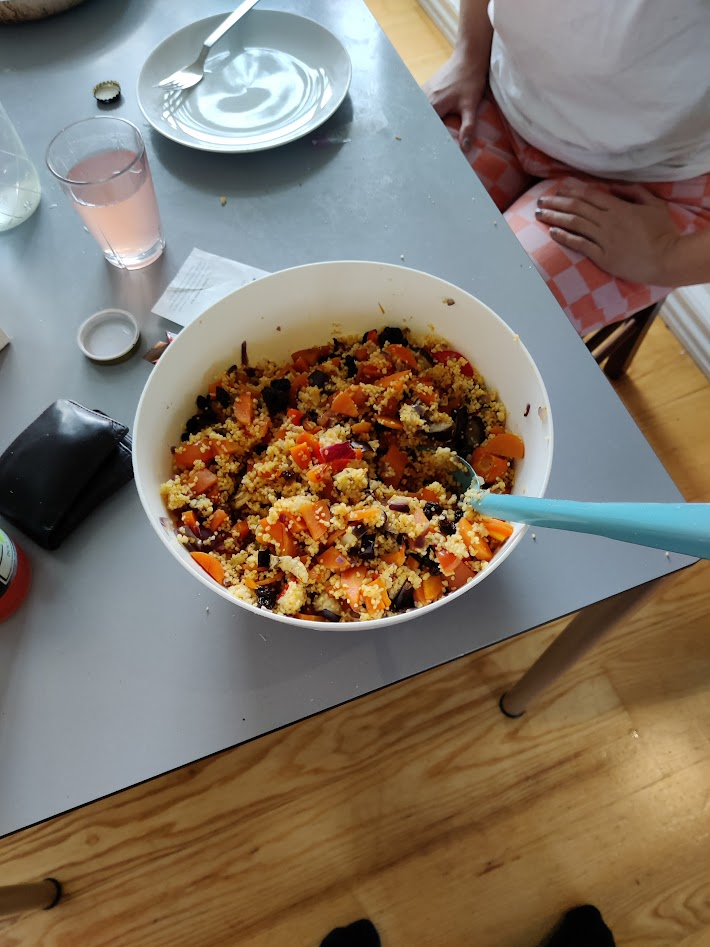
\includegraphics[width=\paperwidth,height=\paperheight]{Billeder/Frokost/Couscous.jpg}
    };
\end{tikzpicture}
\newpage \section{Tun mousse}
\begin{minipage}[t]{0.5\textwidth}
\textbf{Ingredienser:}
\begin{itemize}
    \item 3 dåset tun 
    \item 200g blødt smør
    \item 1 dL cremefraiche
    \item Citronsaft
    \item Salt og peber
\end{itemize}
\end{minipage}
\begin{minipage}[t]{0.5\textwidth}
\textbf{Fremgangsmåde:}
\begin{enumerate}
    \item Blød smørret
    \item Hæld vandet fra tunen, og "riv" tunen fra hinanden til små stykker.
    \item Bland ingredienserne sammen til en blandet masse, og lad stå på køl, helst omkring 6 timer
\end{enumerate}
\end{minipage}
Jeg foretrækker personligt tun i vand, men man kan sikker også bruge tun i olie.

\newpage Her mangler jeg igen et passende billede, så her er et billede af mig klædt ud som en havfrue\begin{figure}
    \centering
    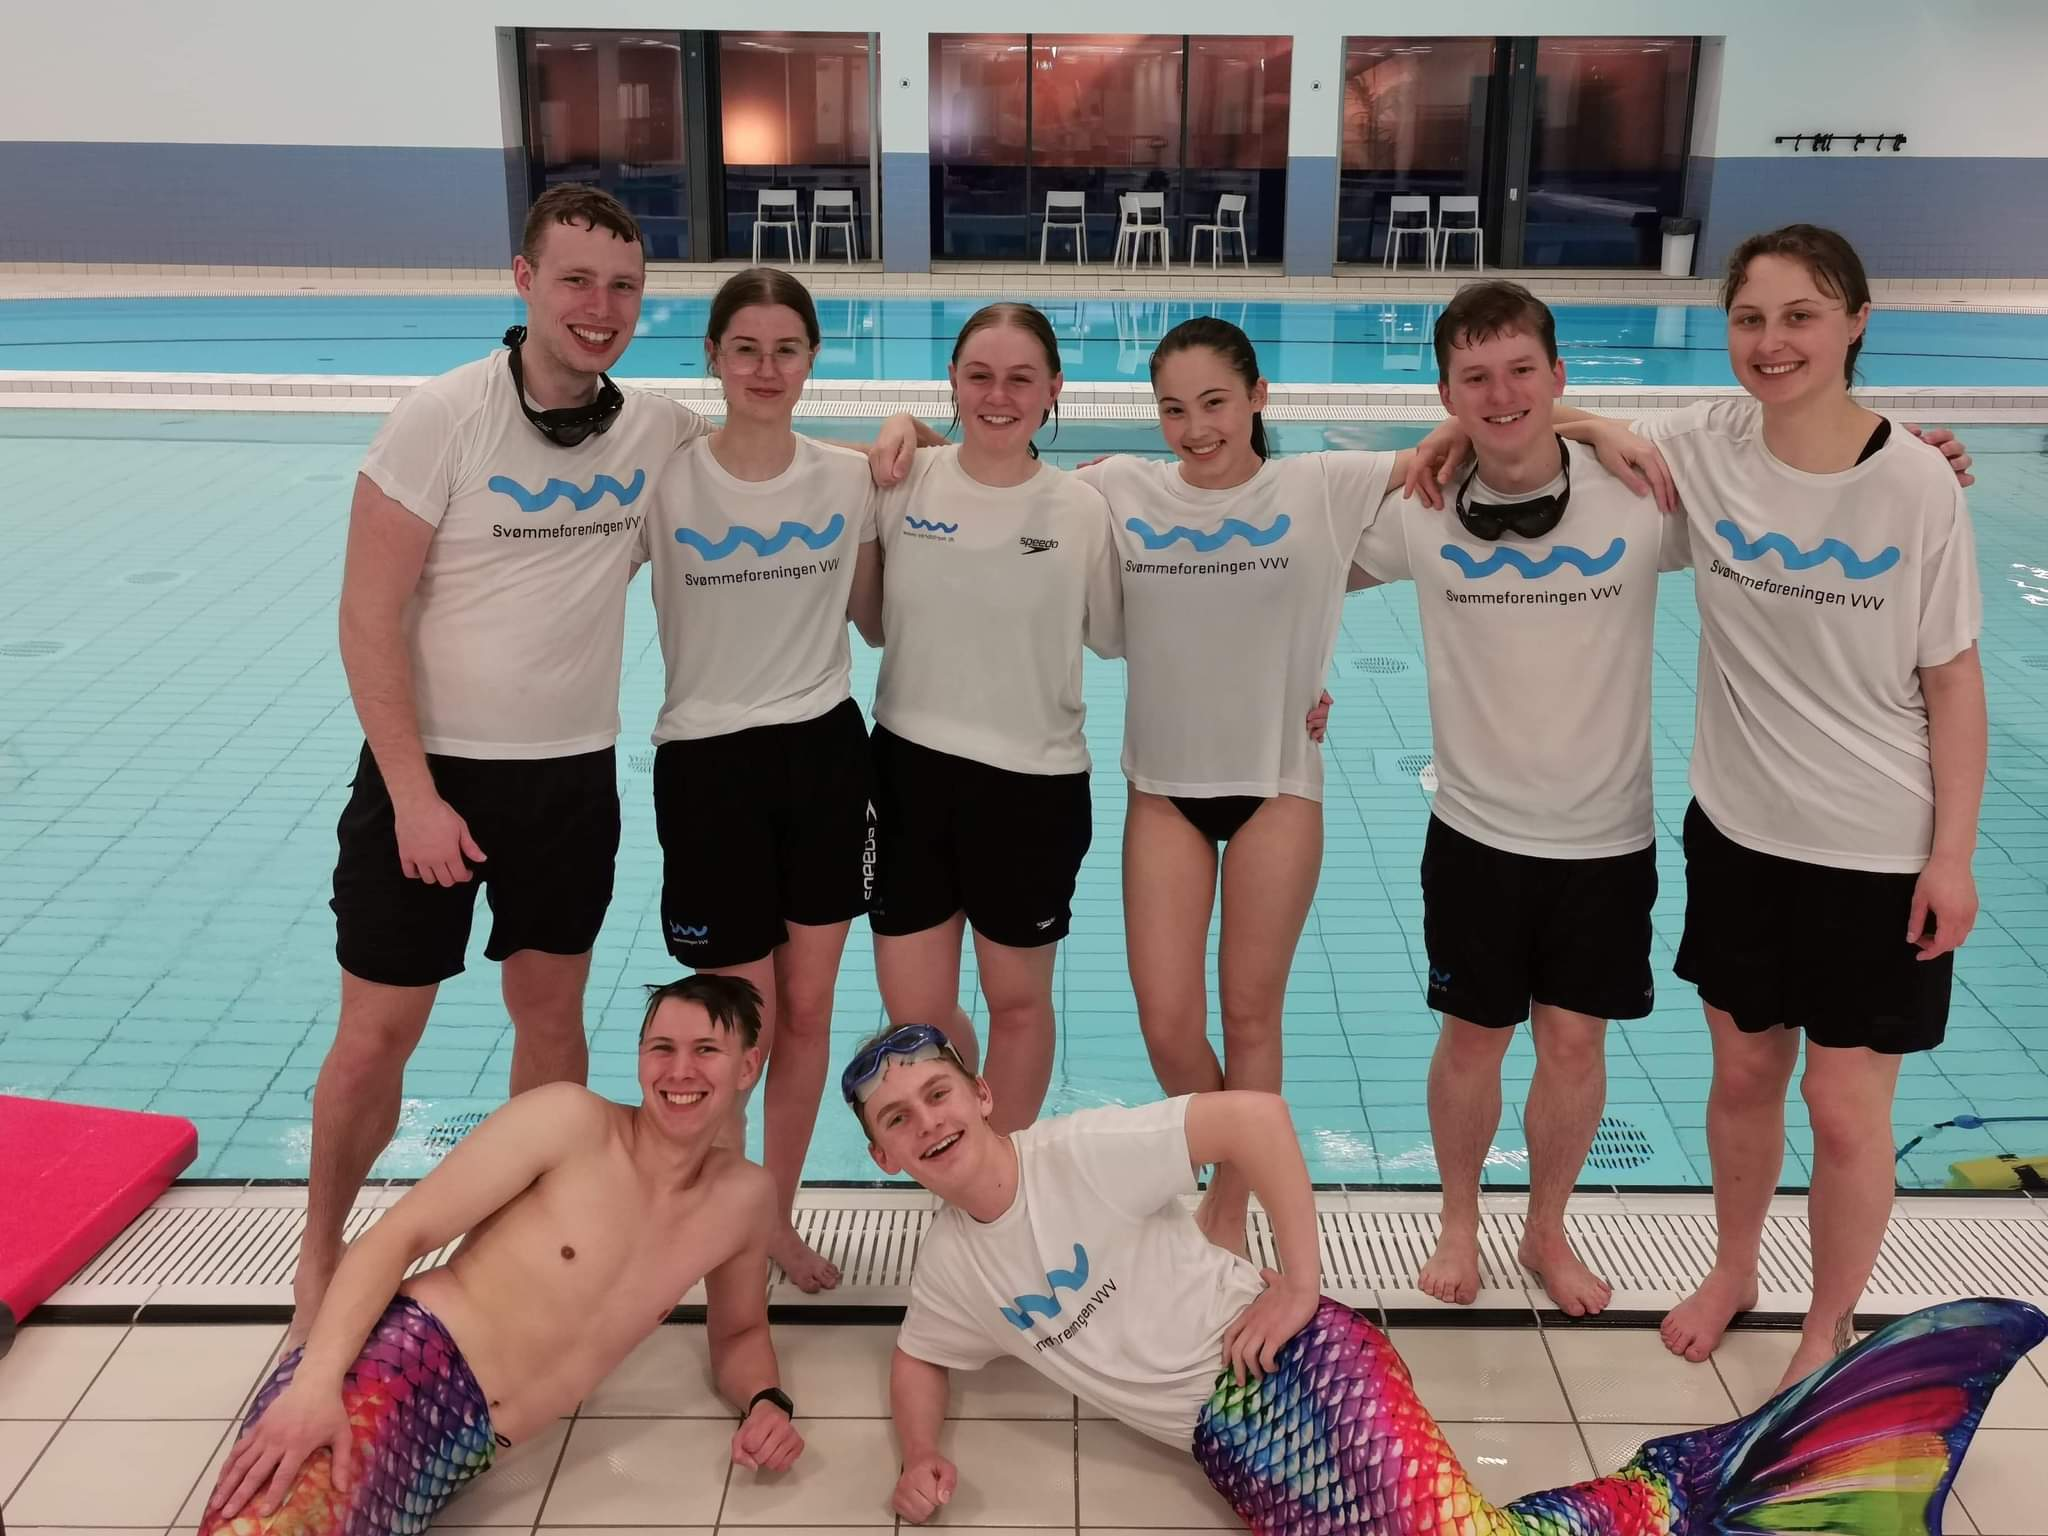
\includegraphics[width=0.75\linewidth]{received_483340176906259.jpeg}
    \caption{VVV coverbillede}
    
\end{figure}
\newpage \section{Vintersalat}
\begin{minipage}[t]{0.5\textwidth}
\textbf{Ingredienser:}
\\ Salaten: 
\begin{itemize}
    \item 150 g belugalinser
    \item 0.25 rødkål, fintsnittet
    \item 1 fennikel, fintsnittet
    \item 1 rødløg, i både
    \item 2 æbler (mellemstore), i små tern
    evt.
    \begin{itemize}
        \item 1 tsk fennikel frø
        \item 1 appelsin, skåret i tern
    \end{itemize}
\end{itemize}
Dressing:
\begin{itemize}
    \item 1 spsk honning
    \item 2 spsk æblecidereddike
    \item 1 tsk Dijon sennep
    \item 4 spsk olivenolie
\end{itemize}
\end{minipage}
\begin{minipage}[t]{0.5\textwidth} 
\textbf{Fremgangsmåde:}
\\ Salaten:
\begin{enumerate}
    \item Kog belugalinserne jævnfør posens henvisning
    \item Lad linserne køle af, mens resten af ingredienserne klargøres.
    \item Bland alle ingredienserne undtagen lidt af æblerne sammen med dressingen.
    \item Drys til sidst resten af æblerne oven på.
\end{enumerate}
Dressingen:
\begin{enumerate}
    \item Bland alle ingredienserne sammen og rør til ensartet konsistens.
    \item Gem lidt af dressingen til serveringen
\end{enumerate}
\end{minipage}
Hvis der ønskes en mere bitter version, kan man eventuelt tilføje mere Dijon sennep.
\newpage  Her skulle der jo helst være et billede af en vintersalat, i stedet for er der et billede af en måges fødder i Oslo, vinter 2018
\begin{figure}
    \centering
    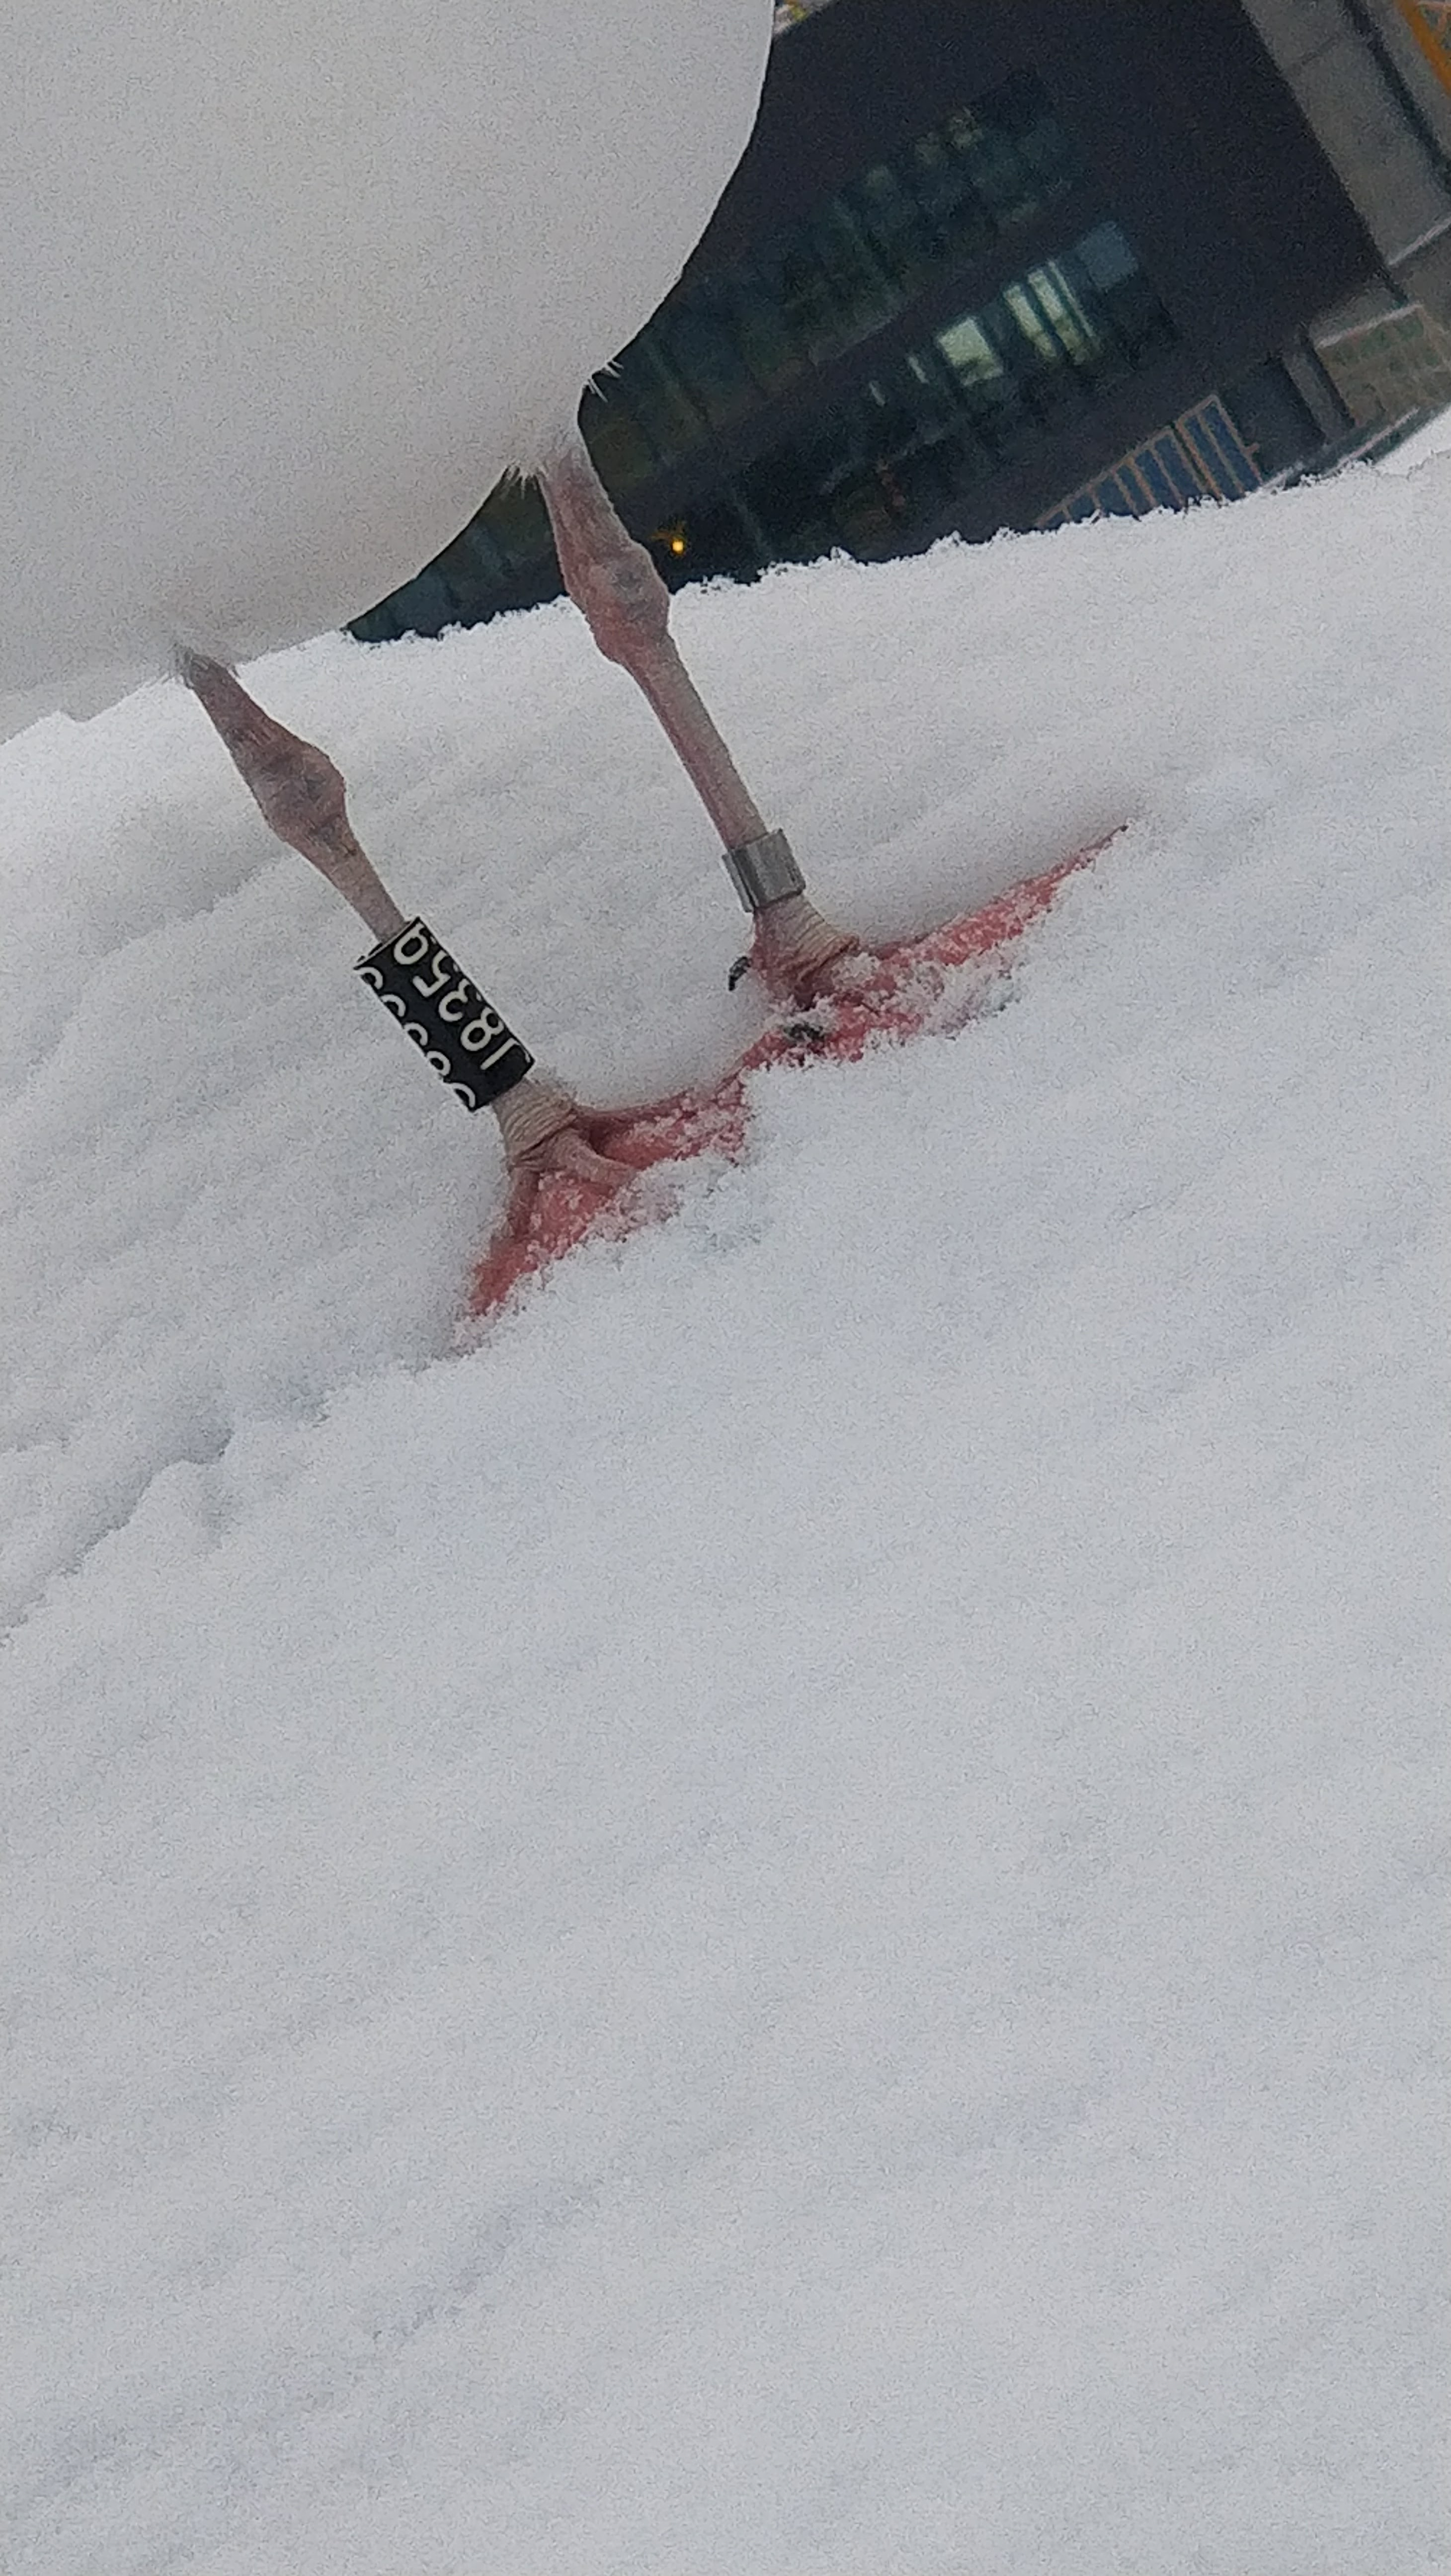
\includegraphics[width=0.5\linewidth]{Måge.jpg}
    \caption{Måge}
    
\end{figure}
\chapter{Ikke Vegetarisk Aftensmad} 
\minitoc
\newpage \section{Andebryststeg}
\begin{minipage}[t]{0.48\textwidth}
\textbf{Ingredienser:}
\begin{itemize}
    \item Optøet andebryststeg (700g)
    \item 25 g smør, blødgjort
    \item Timian
    \item Salt og peber
    \item Rodfrugter (evt øgo rodfrugt mix fra netto)
    \item 2 løg, skåret i både
\end{itemize}
\end{minipage}
\begin{minipage}[t]{0.48\textwidth}
\textbf{Fremgangsmåde:}
\begin{enumerate}
    \item Gnid skindet med en blanding af, blødgjort smør, timian, salt og peber.
    \item Læg anden i et ovnfast fad, med løg og rodfrugter rundt om
    \item Steg anden i forvarmet ovn på 200 \degree C varmluft i 40-45 minutter
    \item Sæt ovnen på grill og skru op på 250 \degree C for at give et sprødt skind, omtrent 5 minutter.
\end{enumerate}
\end{minipage}
\textcolor{white}{Herkujkdansdaskdaskjdhsaidgasdhasiuhdashdbasjkdnasidhbsandusahdbjnashdjkashnidu\\ dsadjiasojdsaodjiasojdasi jdasiojdasioj iasdioas sadasoidas \\}
Efter endt stegning kan man med fordel bruge sovsen i fadet til en brun sovs. Efter min oplevelse er det 40-45 minutter der giver en let rød and, hvis det ønskes gennemstegt, kan man give den lidt mere. Server gerne anden med rodfrugterne eventuelt sammen med kartofler.
Har fundet denne oversigt på nettet over kernetemperatur for and:

\begin{table}[b]
    \centering
    \begin{tabular}{c|c}
         Farve & Kerne temperatur  \\ \hline
         \cellcolor{red!25} Rosa &  62-63 \degree C \\
         \cellcolor{red!35}Let Rosa & 64-65 \degree C   \\
         \cellcolor{brown!40}Gennemstegt & 70-72 \degree C   \\ 
    \end{tabular}
    \caption{Kernetemperatur for stegning af andebryststeg}
\end{table}

\newpage
\begin{tikzpicture}[remember picture,overlay,inner sep=0pt,outer sep=0pt]
    \node[anchor=south east] at (current page.south east) {
        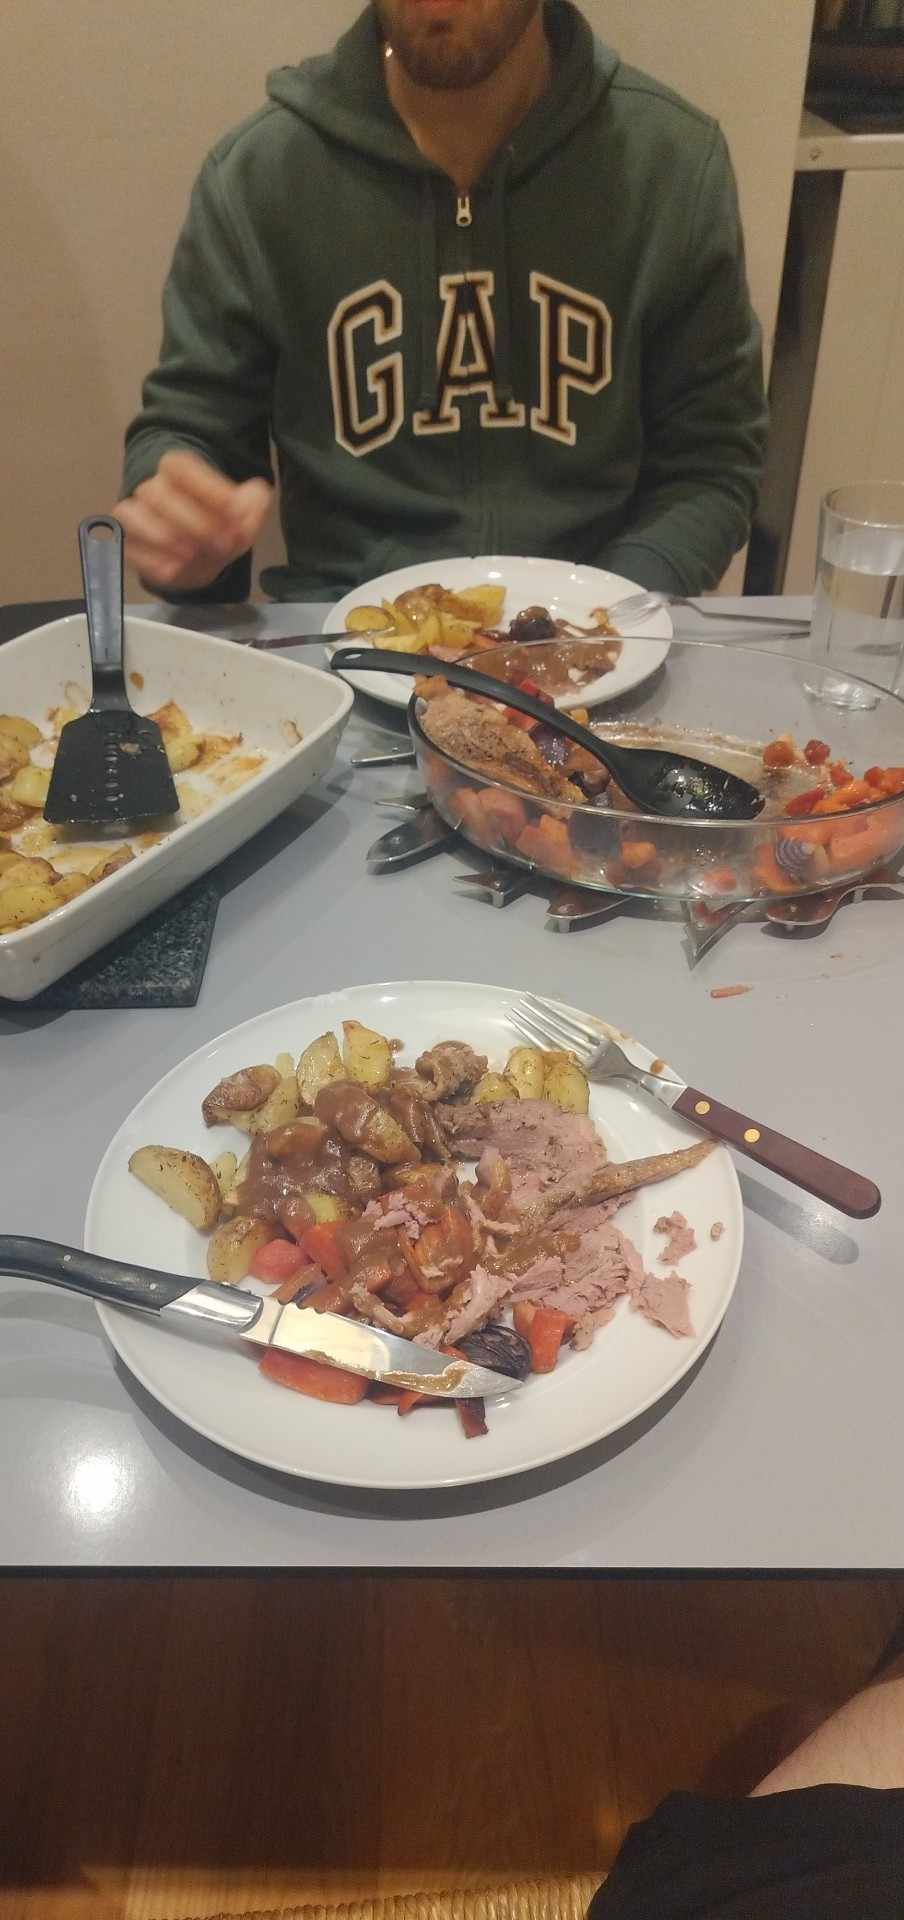
\includegraphics[width=\paperwidth,height=\paperheight]{Billeder/Aftensmad/Andebryststeg.jpeg}
    };
\end{tikzpicture}
\newpage \section{Butter Chicken}
\begin{minipage}[t]{0.5\textwidth}
\textbf{Ingredienser:}
\begin{itemize}
    \item 1-2 løg
    \item 1/2 dL piskefløde
    \item 50g smør
    \item 2spsk olivenolie
    \item 500 g kylling skåret i tynde stykker, kyllingebryst, inderfilet eller lignede
    \item salt og peber
    \item Marinade
    \begin{itemize}
        \item 1 dåse hakkede tomater
        \item 100 g græsk yoghurt (18\% eller 10\%)
        \item 2 tsk chiliflager
        \item 2 tsk stødt spidskommen
        \item 1 tsk stødt kardemomme
        \item 2 tsk garam masala(indisk krydderi blanding)
        \item 2-3 fed hvidløg, presset
        \item 1-2 tsk stødt gurkemejer
        \item 1 tsk tørret ingefær
        \item Evt.
        \begin{itemize}
            \item 1/2 tsk Nellike
            \item 1 tsk Karry
            \item 1 spsk hakket, tørret chilier
        \end{itemize}
    
    \end{itemize}
\end{itemize}
\end{minipage}
\begin{minipage}[t]{0.5\textwidth}
\textbf{Fremgangsmåde:}
\begin{enumerate}
    \item Bland marinaden sammen til en ens masse, og put kylling i, lad stå i køleskabet så længe som muligt.
    \item Skær løgene til ringe.
    \item Smelt smørret, og olien i en gryde og svits løgene til let gennemsigtige.
    \item Tilsæt kyllingen med den tilhørende sovs, samt fløden
    \item Bring det i kog, og lad simre i 30-35 minutter, til kyllingen stort set smuldrer.
\end{enumerate}
\end{minipage}
Til butter chicken skal kylling marinere stort set så længe som muligt, det bliver utroligt mørt hvis man kan give det 24 timer i køleskabet, men smagen kommer også af kortere tid.
\newpage Her skulle der være et billede, har dog ikke kunne finde et så her er et billede af mig der klatrer, indtil jeg laver retten igen.
\begin{figure}
    \centering
    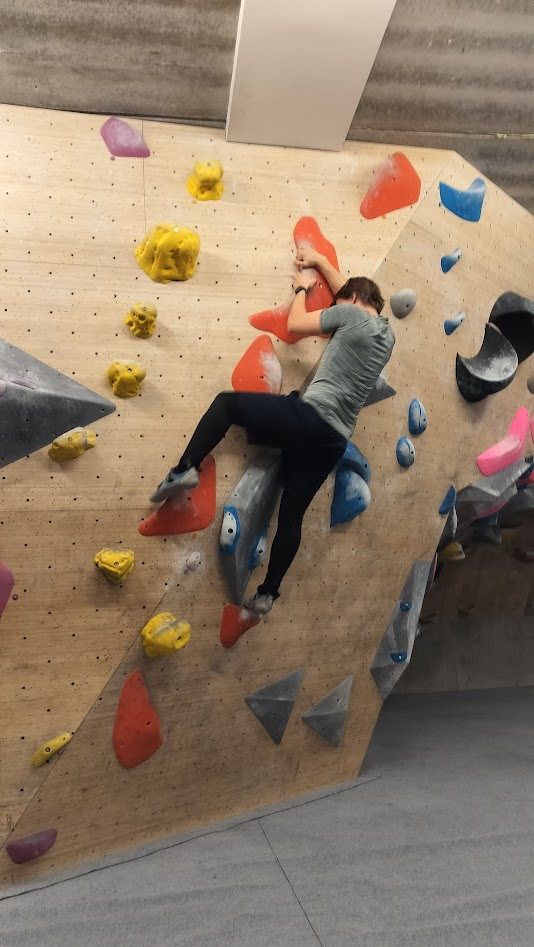
\includegraphics[width=0.5\linewidth]{Klatring.jpg}
    \caption{Mig der klatre, kort tid inden jeg fik svar fra Python eksamen}
    \label{fig:Klatring}
\end{figure}
\newpage \section{Carbonara}
\begin{minipage}[t]{0.5\textwidth}
\textbf{Ingredienser:}
\begin{itemize}
    \item 250 g pasta
    \item 100-150g bacon i tern
    \item 1 tsk smør
    \item 1-2 finthakket løg
    \item 1 dL piskefløde
    \item 2 æg
    \item 75g revet parmesan (eller liggende ost)
    \item Friskkværnet peber
\end{itemize}
\end{minipage}
\begin{minipage}[t]{0.5\textwidth}
\textbf{Fremgangsmåde:}
\begin{enumerate}
    \item Kog pastaen til ønskede konsistens, anbefaler al dente.
    \item Steg baconen, og sæt til siden.
    \item Smelt smørret i en gryde, og svits løgene til gyldne.
    \item Tilsæt bacon og fløde, og lad fløden kortvarigt bruse op .
    \item Skru ned for varmen/fjern fra blusset, og rør æggene samt pastaen i. 
    \item Tilsæt til sidst den revede ost.
\end{enumerate}
\end{minipage}
\newpage
Her mangler jeg igen et billede, så her er der throwback til sommer 2019 til telttur i Sverige.
\begin{figure}
    \centering
    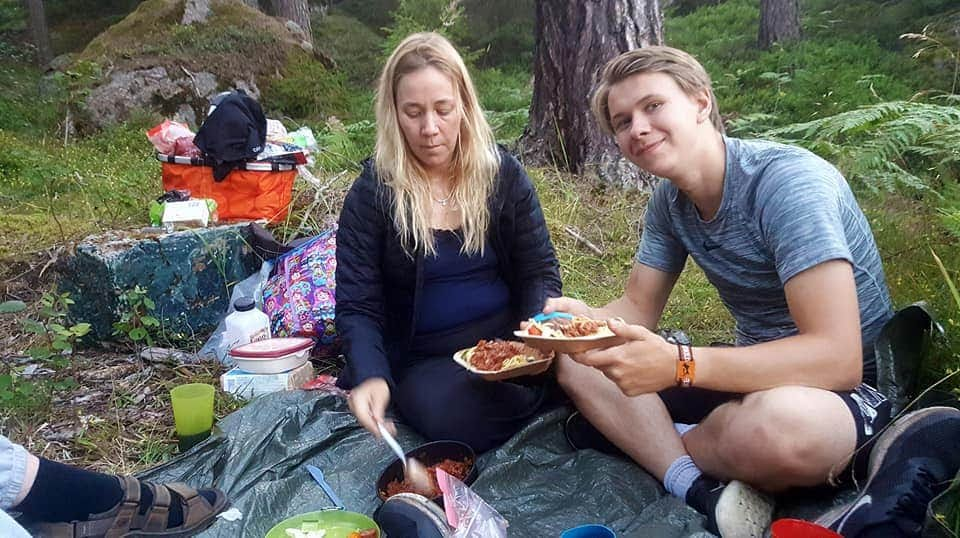
\includegraphics[width=0.5\linewidth]{Skovtur_Sverige.jpg}
    \caption{Mad i Sverige}
    \label{fig:Arbitær 2}
\end{figure}
\newpage \section{Confit De Canard}
\begin{minipage}[t]{0.5\textwidth}
\textbf{Ingrediesner:} 
\begin{itemize}
    \item 2 andelår eller andebryst
    \item 2-3 laurbærblade
    \item Timian
    \item Salt og peber
    \item 500 g andefedt (skal ikke bruges til Sous vide)
\end{itemize}
\end{minipage}
\begin{minipage}[t]{0.5\textwidth}
\textbf{Fremgangsmåde:}
\\ I gryde 
\begin{enumerate}
    \item Gnid anden med timian, salt og peber, og lad marinere natten over i køleskab.
    \item Smelt andefedtet i en gryde, i et lag hvor anden kan helt druknes i fedtet (fedtet skal helst varmes til omtrent 100 \degree C).
    \item Læg anden forsigtigt i, og tilsæt laurbærbladene. 
    \item Kog i mindst 2 timer til kødet er meget mørt (det skal helst rives i stykker med en gaffel).
    \item Når de er godt møre steg anden på panden ved høj varme til at give et crispy finish til skindet.
\end{enumerate}
Sous vide
\begin{enumerate}
    \item Til sous vide er trinene det samme, men frem for at marinere natten over og stege i en gryde, skal den blot have 24-36 timer i sous vide.
    \item Steg også her på panden ved høj varme. 
\end{enumerate}
\end{minipage}
Har endnu ikke kastet mig ud i at sous vide andelår/andebryst, men tænker også det kunne tilføje noget til smagen, hvis man i vakuumposen tilsætte, lidt andefedt, således det steges i dets eget fedt.
\newpage \begin{tikzpicture}[remember picture,overlay,inner sep=0pt,outer sep=0pt]
    \node[anchor=south east] at (current page.south east) {
        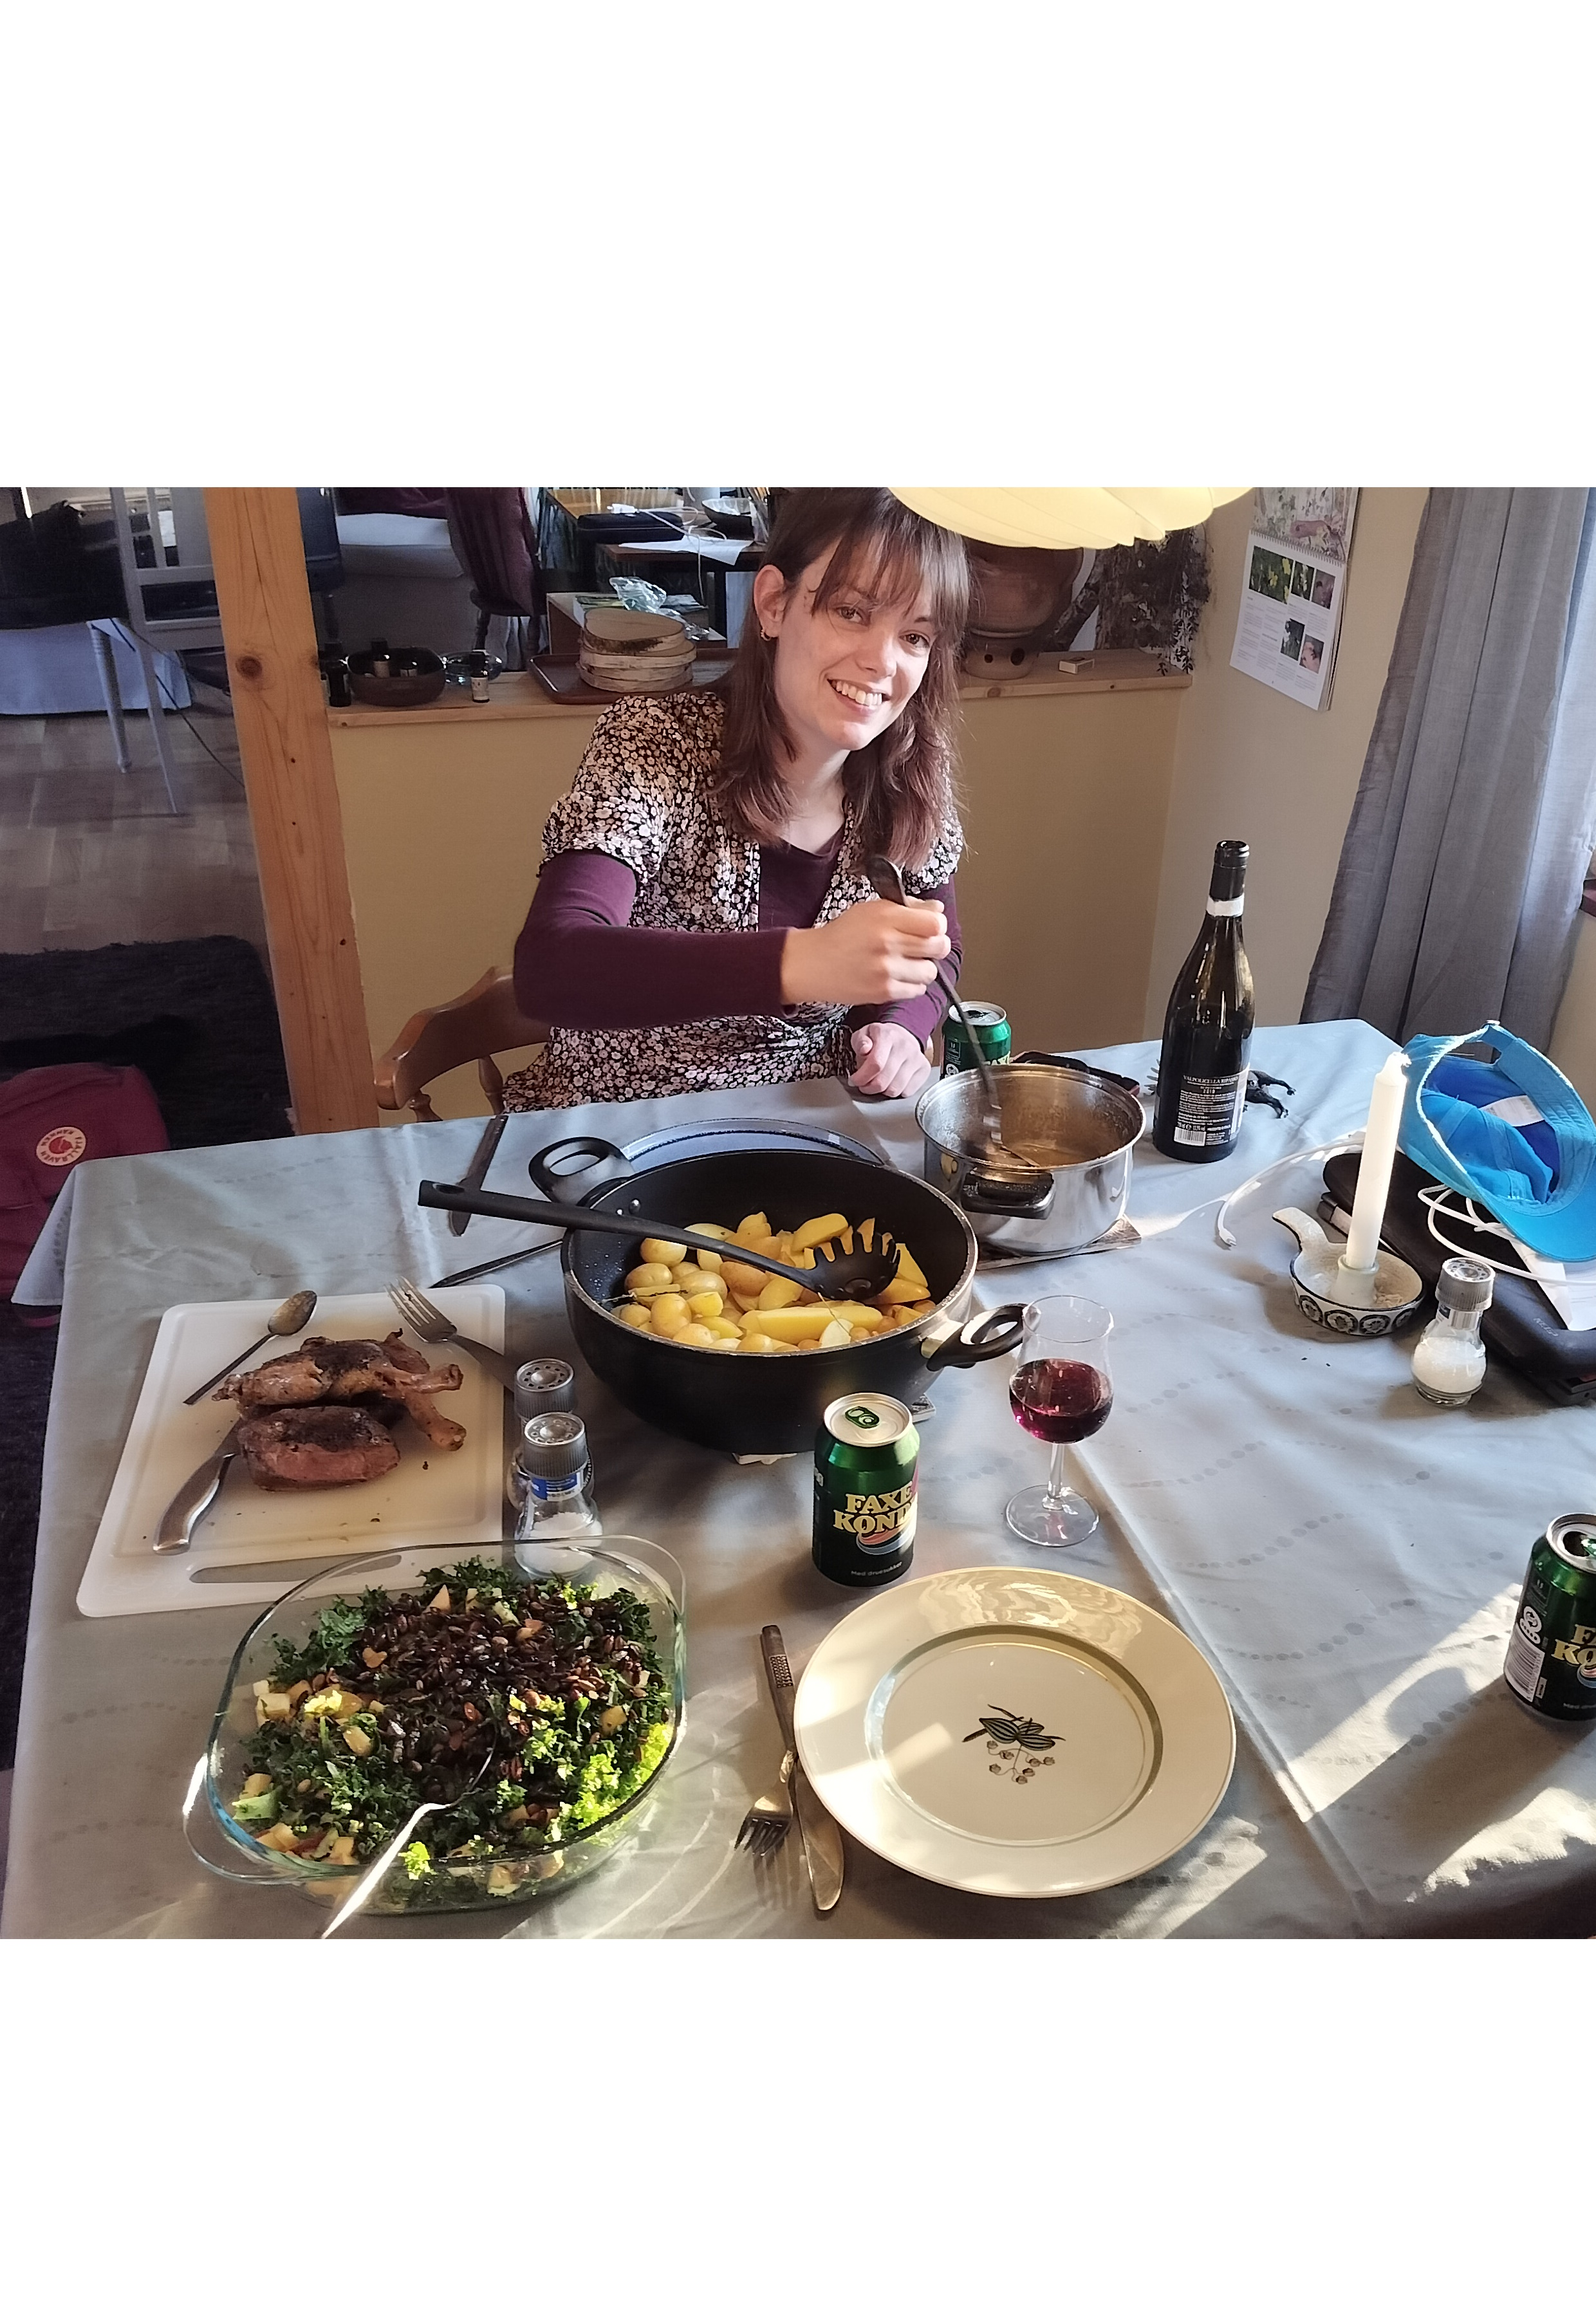
\includegraphics[width=\paperwidth,height=\paperheight]{Billeder/Aftensmad/Confit3.jpg}
    };
\end{tikzpicture}
\newpage \section{Flæskesteg}
\begin{minipage}[t]{0.5\textwidth}
\textbf{Ingredienser}
\begin{itemize}
    \item Flæskesteg, helst med et tykt fedtlag
    \item Flagesalt eller groft salt
    \item Laurbærblade (cirka 1 per 2-3 sværd)
    \item En smule timian
\end{itemize}
\end{minipage}
\begin{minipage}[t]{0.5\textwidth}
\textbf{Fremgangsmåde:}
\begin{itemize}
    \item Rids sværene dybe, til så dybt som muligt, der må ikke ridses ned i selve kødet.
    \item Gnid flæskestegen med krydderierne og fordel laurbærbladene.
    \item Put i ovnen på en rist ovenover en bradepande fyldt med vand og tænd op 175 \degree C. 
    \item Steg til 60 \degree C i midten.
    \item Hvis ikke sværene er blevet så sprøde som forventet, kan man afslutte med 250 \degree C grill.
\end{itemize}
\end{minipage}
\newpage  \begin{tikzpicture}[remember picture,overlay,inner sep=0pt,outer sep=0pt]
    \node[anchor=south east] at (current page.south east) {
        \includegraphics[width=\paperwidth,height=\paperheight]{Billeder/Aftensmad/Flæskesteg.jpg}
    };
\end{tikzpicture}
\newpage \section{Fruta de Mer}
\begin{minipage}[t]{0.5\textwidth}
\textbf{Ingredienser:}
\begin{itemize}
    \item 250g Pasta(jeg fortrækker en form for linguinne)
    \item 250g arabiatta sauce (varierende alt efter hvor tomaterret den skal være)
    \item Skaldyr(rejer, blåmuslinger og hvad man ellers lige har lyst til)
    \begin{enumerate}
        \item Rejer (evt. friske vannamei rejer)
        \item 500 g Blåmuslinger
        \item Evt. Krabbe
        \item Evt. Laks
        \item Evt. Blæksprutte
    \end{enumerate}
    \item Persille og citron til servering
\end{itemize}
\end{minipage}
\begin{minipage}[t]{0.5\textwidth}
\textbf{Fremgangsmåde:}
\begin{enumerate}
    \item Kog pastaen til al dente og sæt til siden.
    \item Klargør de forskellige skaldyr (se eventuel opskrift på Moulles-Frites).
    \item Tilsæt arabiatta saucen til den kogte pasta, og fold ind.
    \item Tilsæt skaldyrene og rør rundt til det er ligeligt fordelt.
    \item Server med persille og citronsaft.
\end{enumerate}
\end{minipage}
\newpage
\begin{tikzpicture}[remember picture,overlay,inner sep=0pt,outer sep=0pt]
    \node[anchor=south east] at (current page.south east) {
        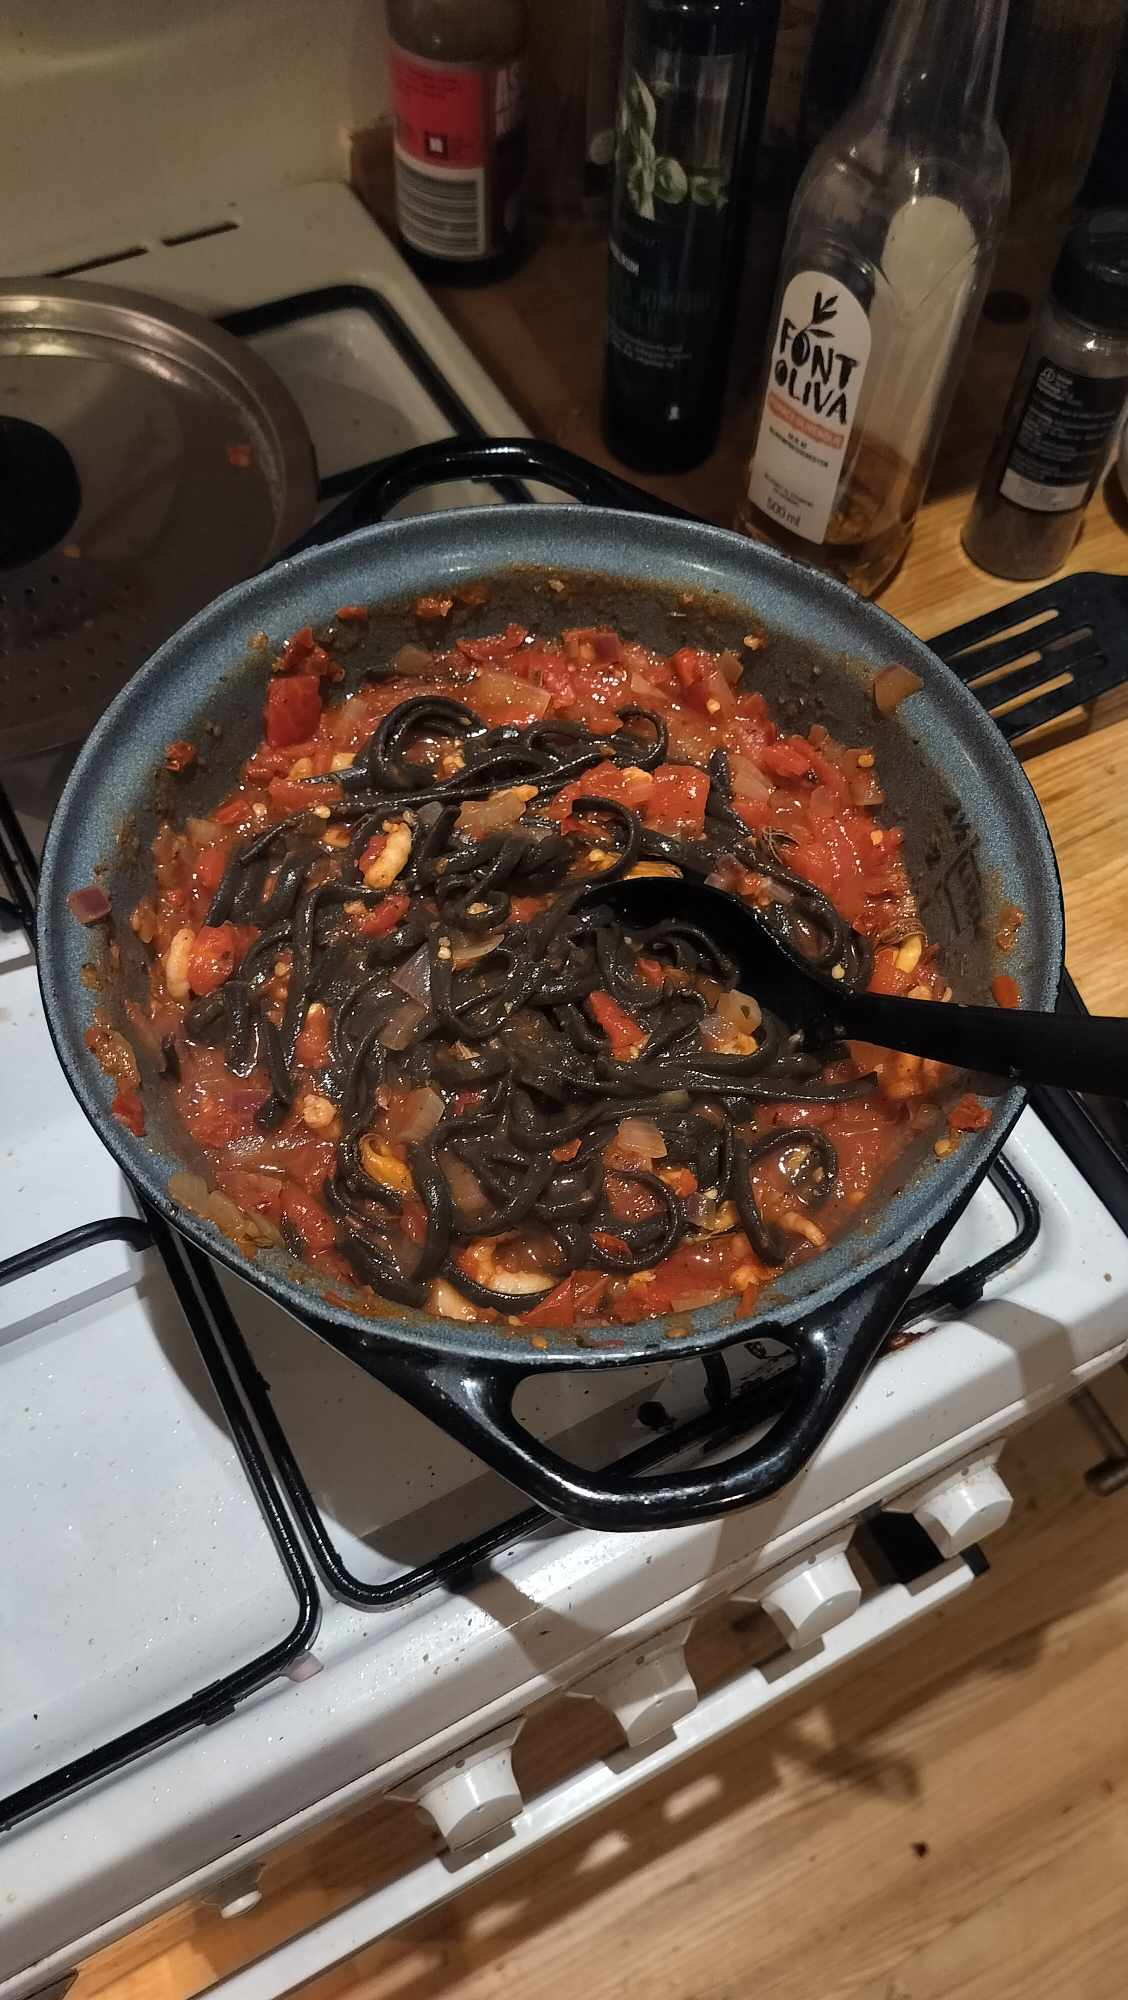
\includegraphics[width=\paperwidth,height=\paperheight]{Billeder/Aftensmad/Fruta_de_mer.jpg}
    };
\end{tikzpicture}
\newpage \section{Laksepasta}
\begin{minipage}[t] {0.5\textwidth}
\textbf{Ingredienser:}
    \begin{itemize}
        \item 250 g frisk pasta
        \item 100 g røget laks
        \item 50-100 g Philadelphia (kommer an på hvor fedtet den skal være)
        \item 2 løg
        Eventuelt
        \begin{enumerate}
            \item Hel bladet spinat
            
        \end{enumerate}
    \end{itemize}
\end{minipage}
\begin{minipage}[t] {0.5\textwidth}
 \textbf{Fremgangsmåde:}
 \begin{enumerate}
     \item Hak løg og grøntsager og steg.
     \item Kog pastaen i 2-3 minutter.
     \item Tøm vandet fra pastaen, og bland alle ingredienserne sammen ved lav varme til en blandet masse.
     
 \end{enumerate}
\end{minipage}
\newpage Her mangler der så også desværre et billede, så i mellemtiden er der et billede af Lord Kelvin og jeg
\begin{figure}
    \centering
    
\includegraphics[width=0.5\linewidth]{Kelvin.jpg}
    \caption{Lord Kelvin }
\end{figure}
\newpage \section{Ovnbagt Laks}
\begin{minipage}[t] {0.5\textwidth}
\textbf{Ingredienser:}
    \begin{itemize}
        \item Lakseside
        \item Porer, skåret i stykker
        \item 2 tomater, skåret i både
        \item rødløg, skåret i 1/4
        \item 1-2 løg, skåret i 1/4
        \item Salt og peber
    \end{itemize}
\end{minipage}
\begin{minipage}[t] {0.5\textwidth}
\textbf{Fremgangsmåde:}
\begin{enumerate}
    \item Hak grøntsagerne, porer i ringe og tomater og løg i både.
    \item Gnid laksesiden med salt og peber, og anbring i fad.
    \item Så vidt muligt så læg grøntsagerne rundt om laksen.
    \item Bag i ovn i 30 minutter ved 175 \degree C.
\end{enumerate}
\end{minipage}
\newpage 
\begin{tikzpicture}[remember picture,overlay,inner sep=0pt,outer sep=0pt]
    \node[anchor=south east] at (current page.south east) {
        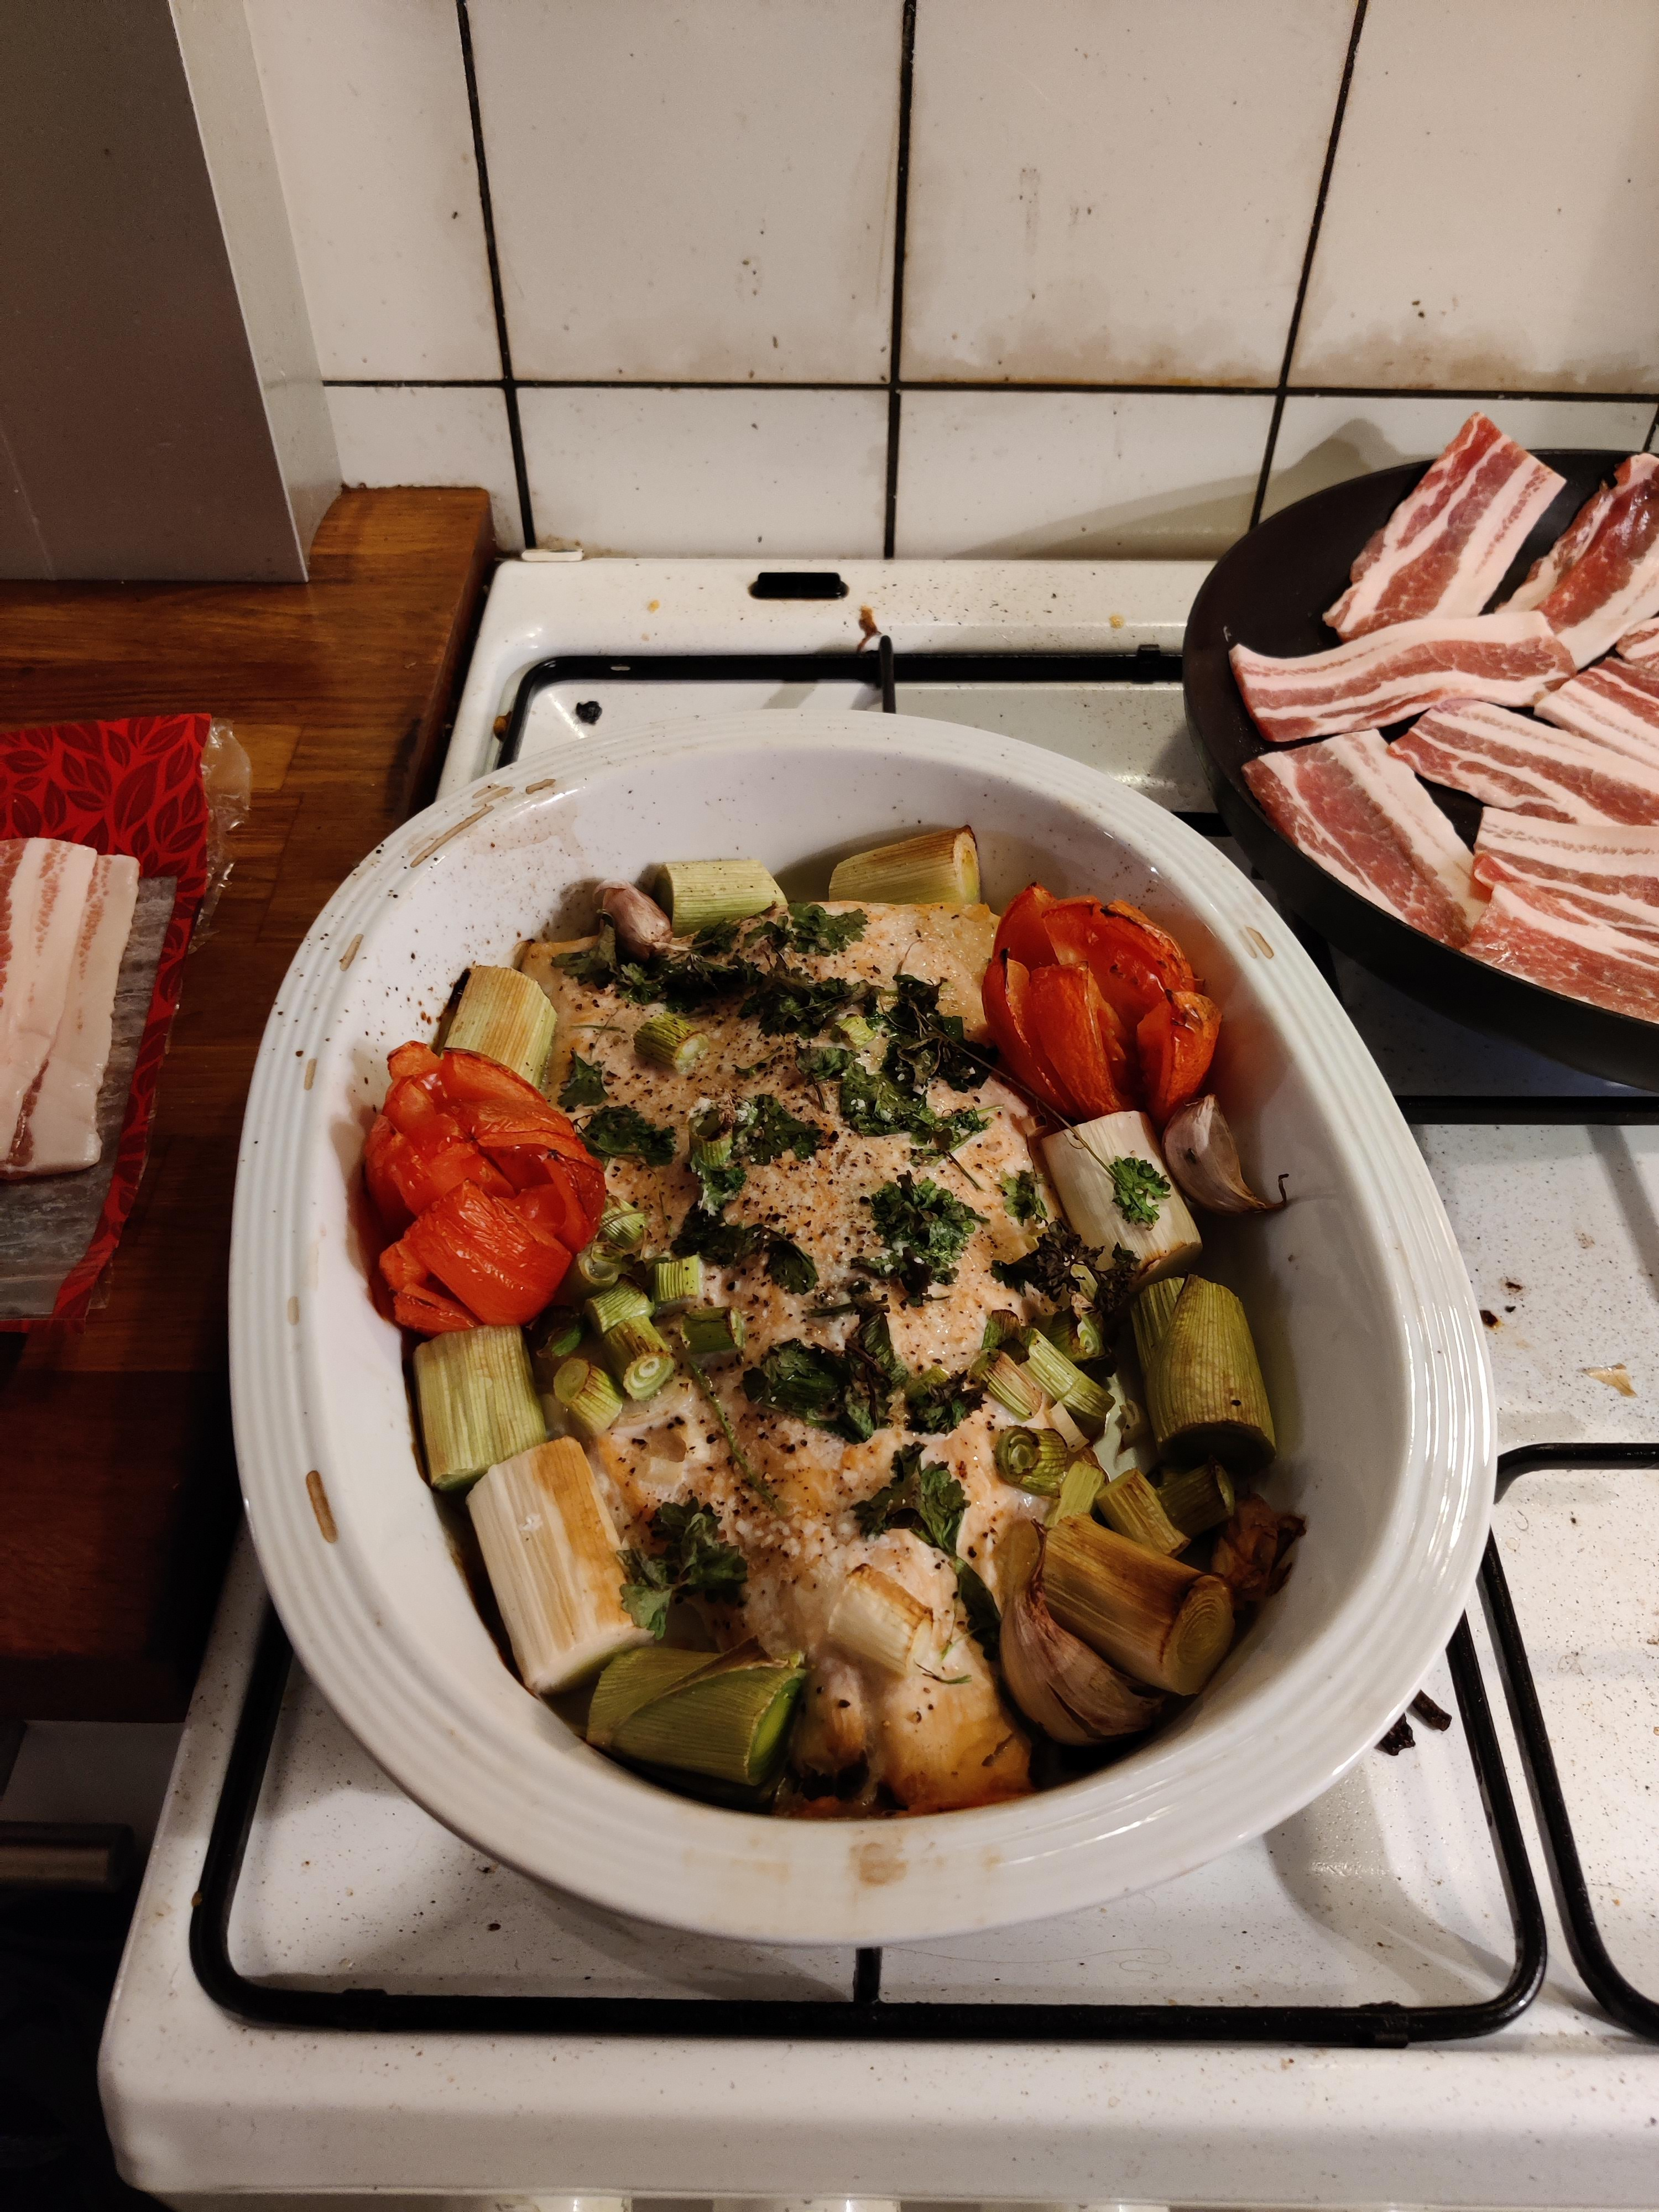
\includegraphics[width=\paperwidth,height=\paperheight]{Billeder/Aftensmad/Ovnbagt_laks.jpg}
    };
\end{tikzpicture}
\newpage \section{Moules Frites}
\begin{minipage}[t]{0.5\textwidth}
\textbf{Ingredienser}
\begin{itemize}
    \item 500g blåmuslinger
    \item 2 tomater
    \item 1 håndfuld koriander
    \item pomfritter
\end{itemize}
\end{minipage}
\begin{minipage}[t]{0.5\textwidth}
\textbf{Fremgangsmåde:}
\begin{enumerate}
    \item Hak tomaterne til tern.
    \item Skær koriander til små stykker.
    \item Skyl blåmuslingerne og sorter de dårlige blåmuslinger fra.
    \item Kog blåmuslinger i en gryde med låg, med tomaterne og korianderne.
    \item Sorter igen de dårlige blåmuslinger fra.
\end{enumerate}
\end{minipage}
\\ \\ \\ 
Når blåmuslinger skal sorteres fra sker det i 2 faser. Før de koges skal de skyles, dem som ikke lukkes er allerede døde og skal frasorteres. Hvis der er synlige skader på blåmuslinger, såsom ødelagt skaller skal disse også sorteres fra. Efter de er kogt, skal de blåmuslinger, som ikke har åbnet sig også sorters fra.
\newpage
\begin{tikzpicture}[remember picture,overlay,inner sep=0pt,outer sep=0pt]
    \node[anchor=south east] at (current page.south east) {
        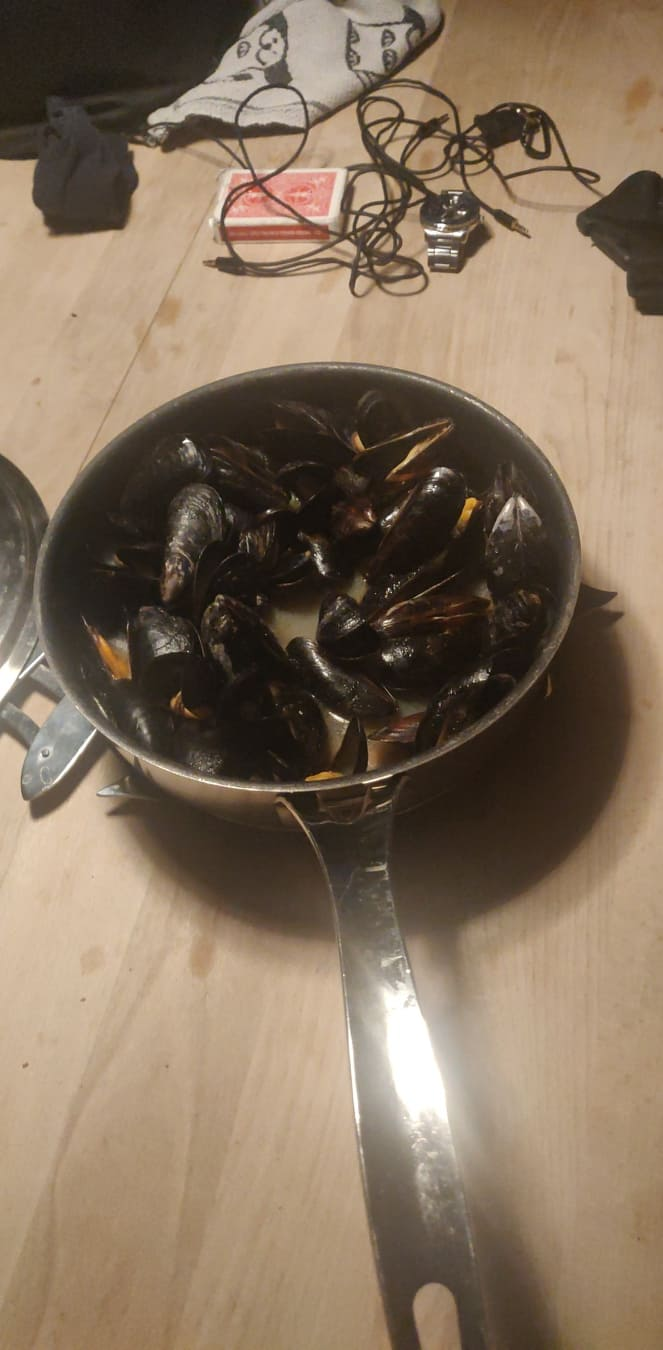
\includegraphics[width=\paperwidth,height=\paperheight]{Billeder/Aftensmad/Moulles_Frittes.jpeg}
    };
\end{tikzpicture}
\newpage \section{Stegt Flæsk med Persillesovs}
\begin{minipage}[t]{0.5\textwidth}
\textbf{Ingredienser:}
\begin{itemize}
    \item 700g flæsk i skiver
    \item 2 spsk hvedemel
    \item 5 dL mælk
    \item 1/2 citron, saft og skal herfra
    \item 2-3 håndfulde persille, finthakket
\end{itemize}
\end{minipage}
\begin{minipage}[t]{0.5\textwidth}
\textbf{Fremgangsmåde:}
\\Flæsken:
\begin{enumerate}
    \item Drys salt over flæsket, og læg på en rist
    \item Steg flæsket i ovn ved 175 \degree C varmluft, og vend helst undervejs.
\end{enumerate}
Persillesovsen:
\begin{enumerate}
    \item Smelt smørret ved lav varme og pisk melet i, lidt efter lidt.
    \item Pisk mælken i ligeså.
    \item Kog saucen ved middel varme i cirka 5 minutter.
    \item Tilsæt det finthakkede persille.
    \item Smag til med salt, peber og citron.
\end{enumerate}
\end{minipage}
OBS. For at undgå et rod, anbefaler jeg at man beklæder en bradepande med bagepapir, som kan stå i bunden i ovnen.
\newpage 
\begin{tikzpicture}[remember picture,overlay,inner sep=0pt,outer sep=0pt]
    \node[anchor=south east] at (current page.south east) {
        \includegraphics[width=\paperwidth,height=\paperheight]{Billeder/Aftensmad/Stegt_Flæsk_Med_Persille_Sovs.jpeg}
    };
\end{tikzpicture}
\newpage \section{Stegte Ris}
\begin{minipage}[t]{0.5\textwidth}
\begin{itemize}
    \item 200g kogte ris
    \item 200g blandede grøntsager(vegetable mix eller wok mix fra Netto)
    \item 100g mukimmame bønner
    \item Ekstra fyld
     \begin{itemize}
        \item evt. Flere grøntsager hvis ønsket
        \item evt. Pandestegt spidskål (eventuelt stegt i gochujang(koreansk chili pasta))
        \item 100g kylling
    \end{itemize}
    \item Smør til stegning
    \item Soja til stegning
    \item 1 æg til stegning
\end{itemize}
\end{minipage}
\begin{minipage}[t]{0.5\textwidth}
\textbf{Fremgangsmåde:}
\begin{enumerate}
    \item Klargør grøntsagerne, tø grøntsager op, steg spidskålet osv, og steg kyllingen.
    \item Smør siden af en wok med smør, og put risene i ved høj varme.
    \item Tilsæt æg, til risene og rør grundigt rundt, det vigtigt at æggene ikke bliver spejlet.
    \item tilsæt grøntsagerne, kyllingen og sojasaucen og steg under omrøring.
    \item Når risene har fået en brun farve, og ikke er klistret, er de good to go.
\end{enumerate}
\end{minipage}
\newpage   Her har jeg igen glemt at tage et billede, så i mellemtiden er der et billede af mig på en sushi restaurant  \begin{figure}
    \centering
    
\includegraphics[width=0.5\linewidth]{Sushi_spisning.jpg}
    \caption{Et billede af mig på CC sushi restaurant  på Åboulevarden}
\end{figure}
\newpage \section{T'uhu}
Sumerisk lam og rødbede gryderet, som er den ældste kendte opskrift, estimeret at være flere tusind år gammel. 

\begin{minipage}[t]{0.5\textwidth}
\textbf{Ingredienser:}
\begin{itemize}
    \item 500g Fedtrigt lam i tern (Egentlig fårekød men det pænt svært at få)
    \item 100 mL får fedt (eller kokosolie da får fedt også er svært at anskaffe)
    \item 1 løg
    \item 1 tsk salt
    \item 500g rødbeder i tern
    \item 100g hakket rucola
    \item Frisk koriander
    \item 125g hakket skalotteløg
    \item 1 tsk spidskommen frø
    \item 100mL Weissbier
    \item 50 mL vand
    \item 75g hakket porrer
    \item 3 fed hvidløg
\end{itemize}
\underline{Tilbehør:}
\begin{itemize}
    \item 75g friske hakkede koriander
    \item 75g forårsløg
    \item 2 tsk spidskommen frø
\end{itemize}
\end{minipage}%
\begin{minipage}[t]{0.5\textwidth}
\textbf{Fremgangsmåde:}
\begin{enumerate}
    \item Varm kokosolie (eller andet fedt) i en gryde bred nok til det hakkede lam, i et lag.
    \item Svits lammet indtil al væsken er væk.
    \item Tilsæt løgene og steg indtil de er gennemsigtige.
    \item Tilsæt derefter salt, rødbeder, rucola, koriander, skalotteløg og spidskommenfrø, og steg indtil væsken er væk.
    \item Tilsæt øllen, vandet og bring det i kog.
    \item Tilføj løg og porrer og lad det simre i en times tid.
\end{enumerate}
\underline{Tilbehør:}
\begin{enumerate}
    \item Knus forårsløgene og korianderne i en morter eller lignende og drys spidskommenfrøene på.
\end{enumerate}
\end{minipage}
\footnote{Kilde: \href{https://www.bbc.com/travel/article/20191103-the-worlds-oldest-known-recipes-decoded}{BBC travel}}
\newpage
\begin{tikzpicture}[remember picture,overlay,inner sep=0pt,outer sep=0pt]
    \node[anchor=south east] at (current page.south east) {
        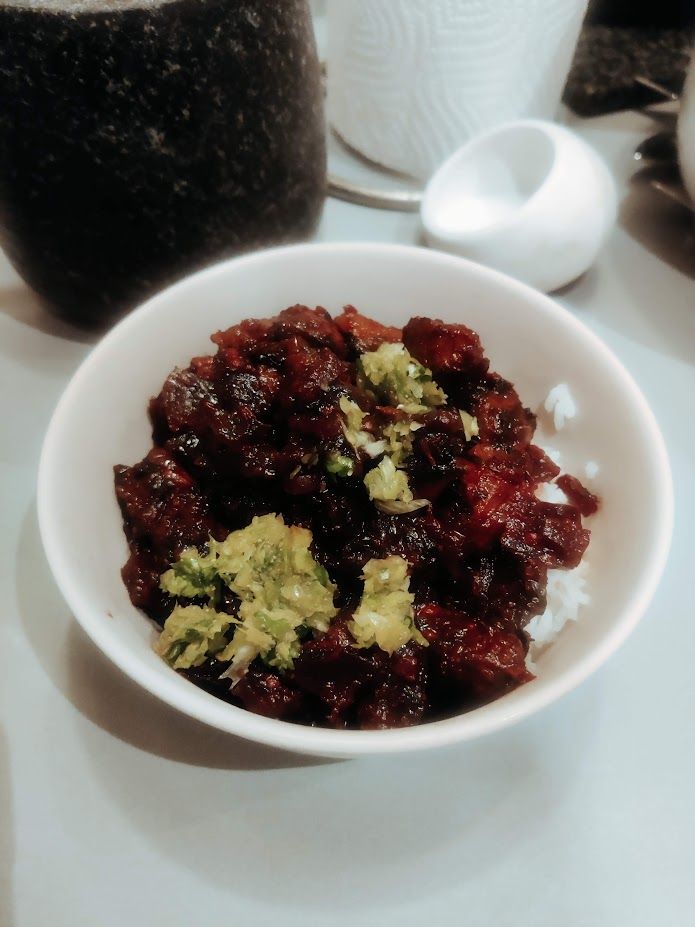
\includegraphics[width=\paperwidth,height=\paperheight]{Billeder/Aftensmad/Tuhu.jpg}
    };
\end{tikzpicture}
\chapter{Vegetarisk Aftensmad}
\minitoc 
\newpage \section{Arabiatta}
\begin{minipage}[t]{0.5\textwidth}
\textbf{Ingredienser:}
\begin{itemize}
    \item 1 dåse flåede tomater
    \item 3 spsk olivenolie
    \item 1 tsk balsamico
    \item 1 tsk sukker
    \item Citronsaft
    \item 1-2 håndfuld basilikum
    \item 1/2 tsk chiliflager 
    \item 2-3 presset fed hvidløg
    \item 1 finthakket løg
\end{itemize}
\end{minipage}
\begin{minipage}[t]{0.5\textwidth}
\textbf{Fremgangsmåde:}
\begin{enumerate}
    \item Svits løgene i olien.
    \item Tilsæt hvidløg, tomater, sukker og basilikum.
    \item Smag til med balsamico, salt og peber
\end{enumerate}
\end{minipage}
\newpage Her mangler der så også et billede desværre, så her er endnu et billede fra Sverige turen.
\begin{figure}
    \centering
    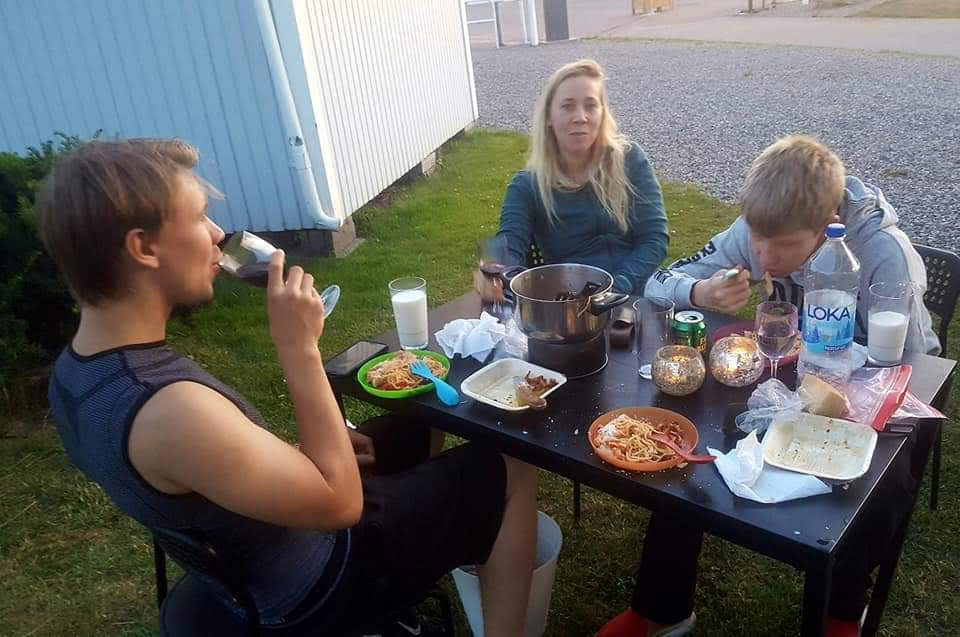
\includegraphics[width=0.5\linewidth]{Sverigept1.jpg}
    \caption{Sverige pt 1}
    
\end{figure}
\newpage \section{Brasede Kartofler}
\begin{minipage}[t]{0.5\textwidth}
\textbf{Ingredienser:}
\begin{itemize}
    \item 1 kg skyllet kartofler
\item 50 g smeltet smør eller 3 spsk olivenolie
\item Timian
\item Salt og peber
\end{itemize}
\end{minipage}
\begin{minipage}[t]{0.5\textwidth}
\textbf{Fremgangsmåde:}
\begin{enumerate}
    \item Skær kartoflerne i skiver (omtrent 1 cm tykke).
\item Anret dem i et ovnfast fad, og dæk med smør(eller olie).
\item Bag i varmlufts ovn ved 180 \degree C, i 40 – 45 minutter, for rå kartofler.
\item Undervejs skal kartoflerne vendes lidt, de skal, efter min smag, være lidt mørkebrune.
\end{enumerate}
\end{minipage}
Til opskriften kan der både bruges allerede kogte kartofler, og rå kartofler, til de rå kartofler skal der markant mindre tid til at braisere dem. 
\\ Passene til frokost, dagen derpå.
\\ \underline{Samlet tid: 1 time}

\newpage \begin{tikzpicture}[remember picture,overlay,inner sep=0pt,outer sep=0pt]
    \node[anchor=south east] at (current page.south east) {
        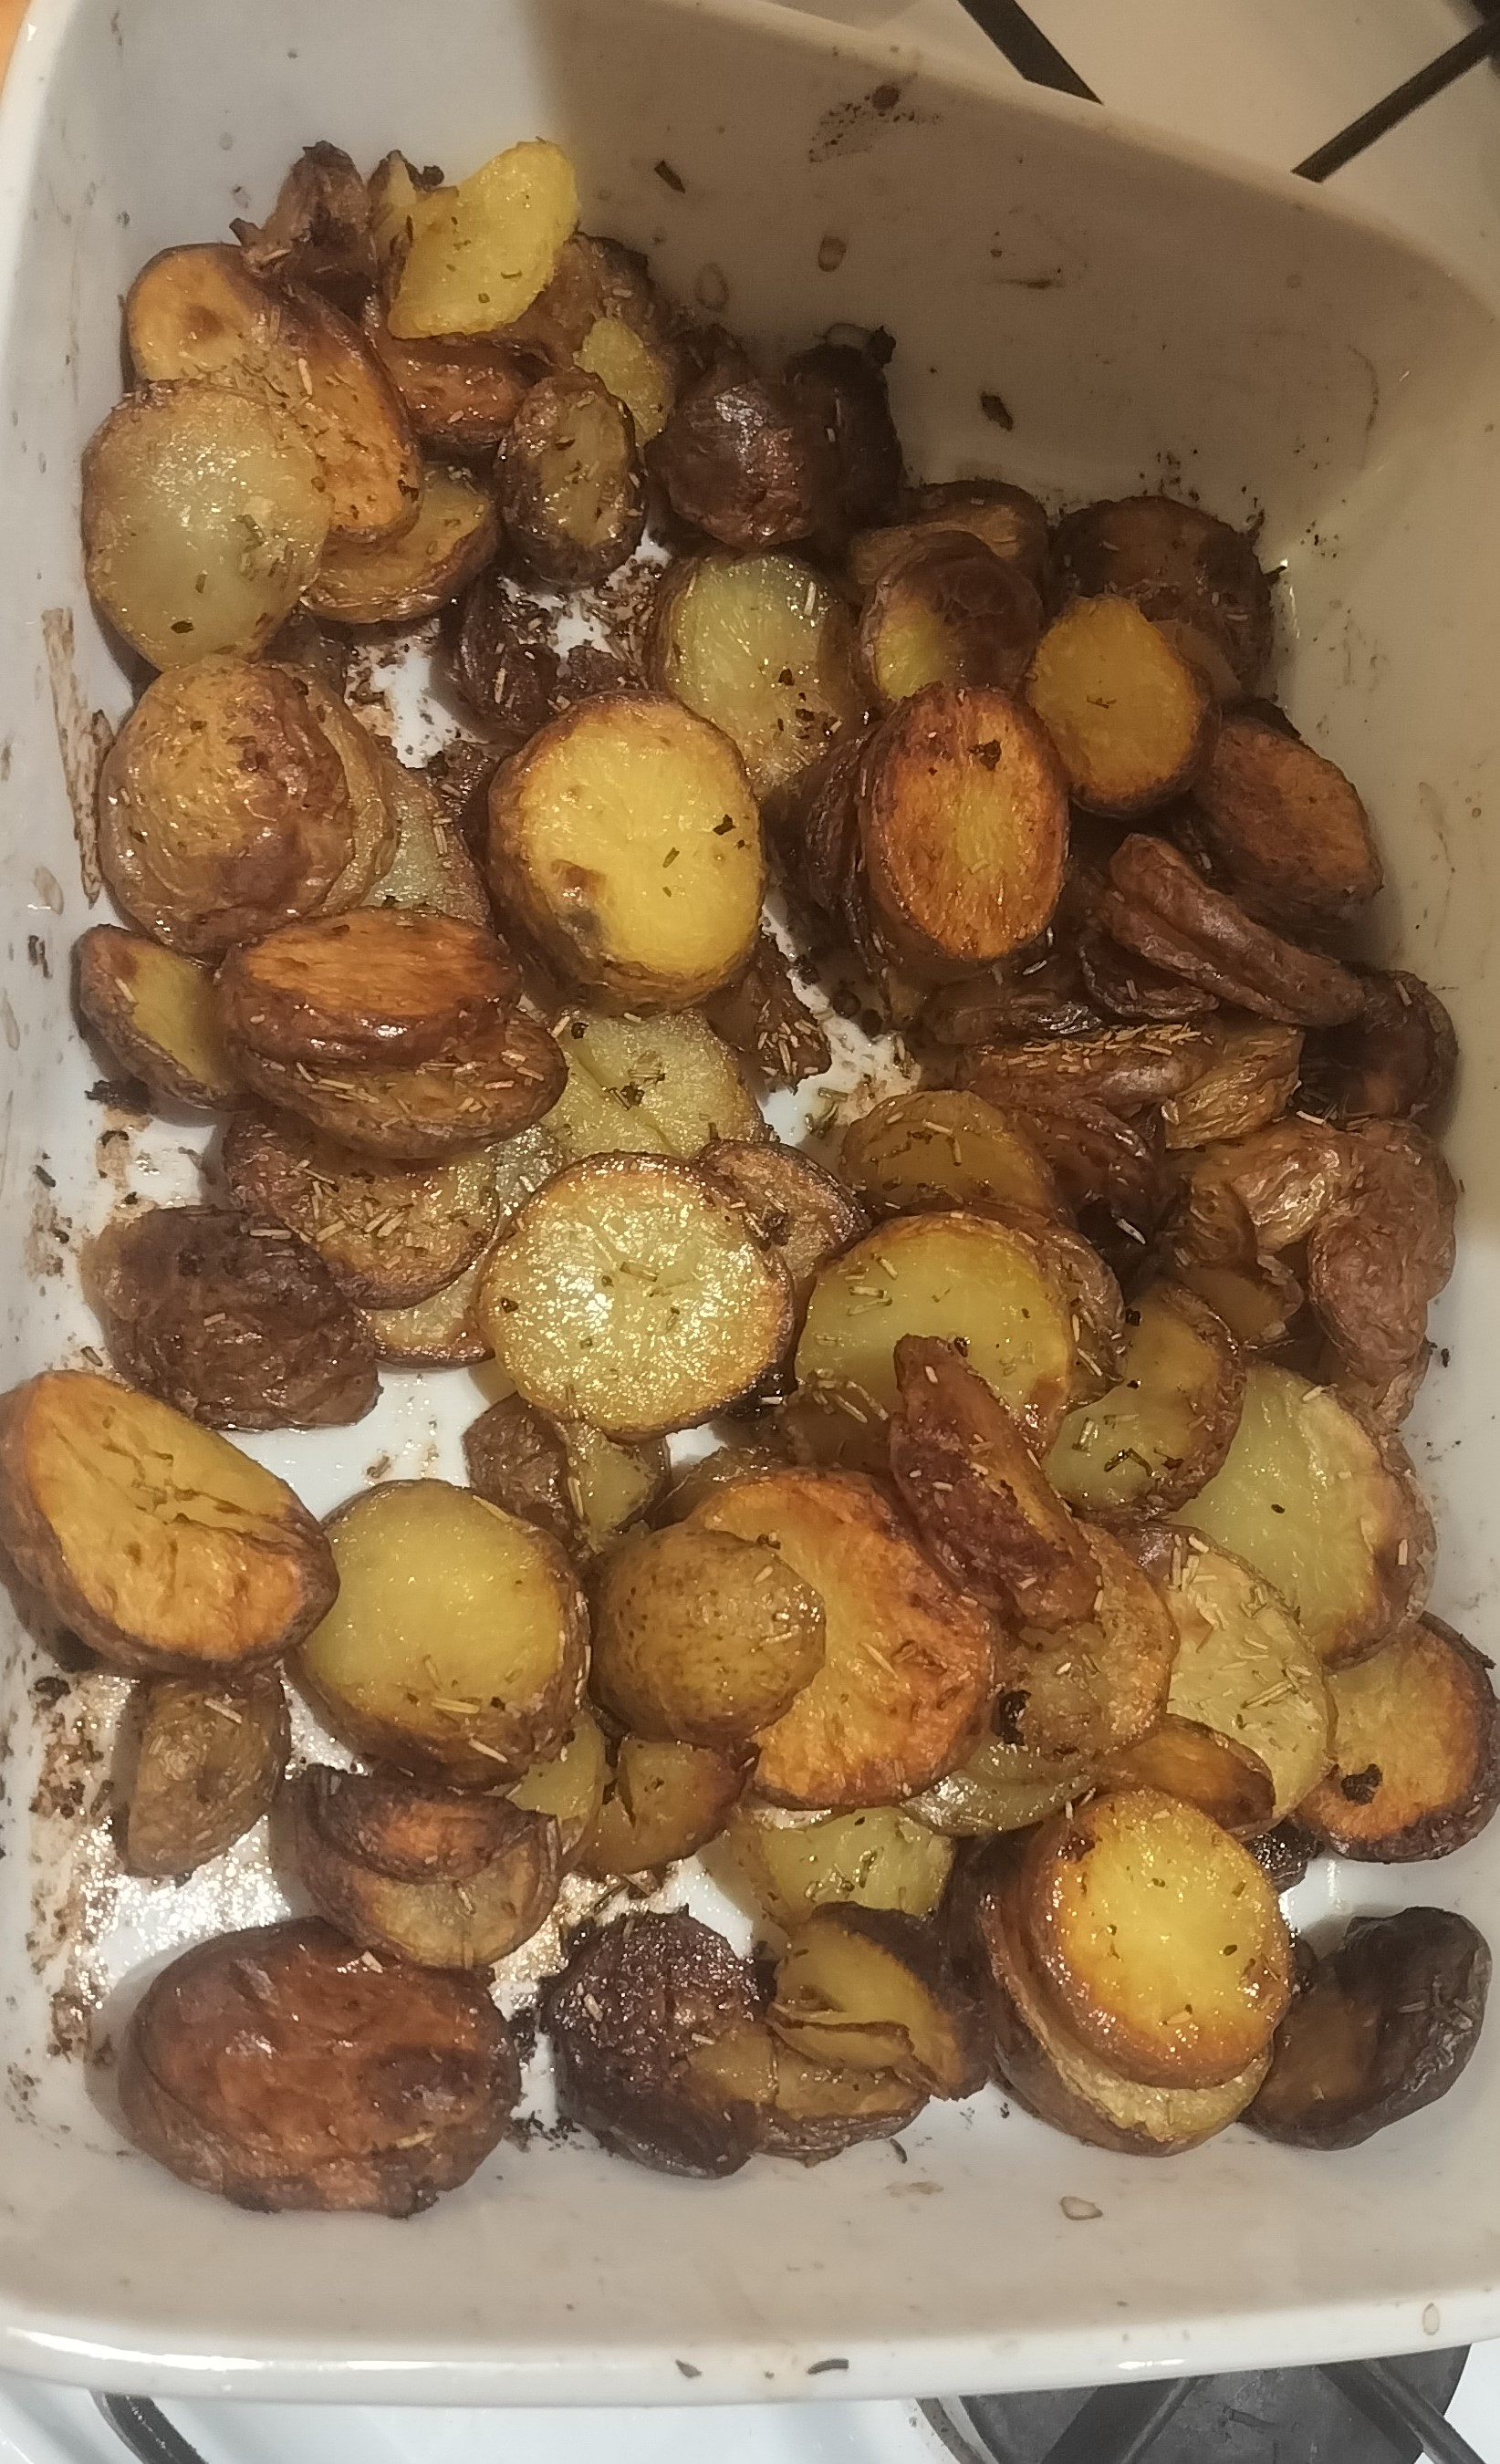
\includegraphics[width=\paperwidth,height=\paperheight]{Billeder/Aftensmad/Brasede_Kartofler2.jpg}
    };
\end{tikzpicture}
\newpage \section{Dhal}
\begin{minipage}[t]{0.5\textwidth}
\textbf{Ingredienser} \\
\underline{Dhal}
\begin{itemize}
    \item 4 fed hvidløg
    \item 2 løg
    \item 2 spsk frisk revet ingefær, eller 2 tsk tørret
    \item 2 spsk olivenolie
    \item 200 gram tørre røde linser
    \item 2 dåser hakkede tomater
    \item Krydderier
    \begin{enumerate}
        \item 6 dL grøntsagsbouillon
        \item 0.5 tsk chiliflager
        \item 0.5 tsk stødt kardemomme
        \item 0.5 spsk stødt koriander
        \item 1 spsk stødt spidskommen
        \item 0.5 tsk garam masala(indisk krydderi blanding) 
        \item 0.5 tsk paprika
    \end{enumerate}
    \end{itemize} 
\underline{Raita:}
\begin{itemize} 
    \item 1 håndfuld mynte
    \item 2 dL græsk yoghurt 10\%
    \item 0.5 agurk, mandolin revet
    \item 2 fed hvidløg
    \item spidskommen
    \item salt og peber
    \item Eventuelt
    \begin{itemize}
        \item Citronsaft eller limesaft
    \end{itemize}
\end{itemize}
\end{minipage}
\begin{minipage}[t]{0.5\textwidth}
\textbf{Fremgangsmåde:} \\
\underline{Dhal} 
\begin{enumerate}
    \item Svits løg, hvidløg og krydderier i olien.
    \item Tilsæt, grøntsagsbouillon, vaskede linser og de hakkede tomater.
    \item Bring op og koge, og lad simre i mindst 30 minutter, konsistensen kan reddes med eventuel flere linser (hvis den er for flydende) eller mere vand (hvis den er for fast). Smag til med salt og peber.
\end{enumerate}
\underline{Raita:}
\begin{enumerate}
    \item Riv agurken i tykke skive og dræn vandet derfra.
    \item Skær mynten i små stykker.
    \item Mix ingredienserne sammen og smag til med salt og peber.
\end{enumerate}
\end{minipage}
\\ \\ \\ \underline{Noter:}
Der kan sagtens bruges våde linser (fra en dåse), men så skal der bruges markant mindre væske. \\ Til servevingen kan den pyntes med friske koriander, eller eventuelt ristede græskarkerner.  \\ Dhal kan sagtens spises for sig selv, men kan også nydes med enten naan brød, eller ris.


\newpage
\begin{tikzpicture}[remember picture,overlay,inner sep=0pt,outer sep=0pt]
    \node[anchor=south east] at (current page.south east) {
        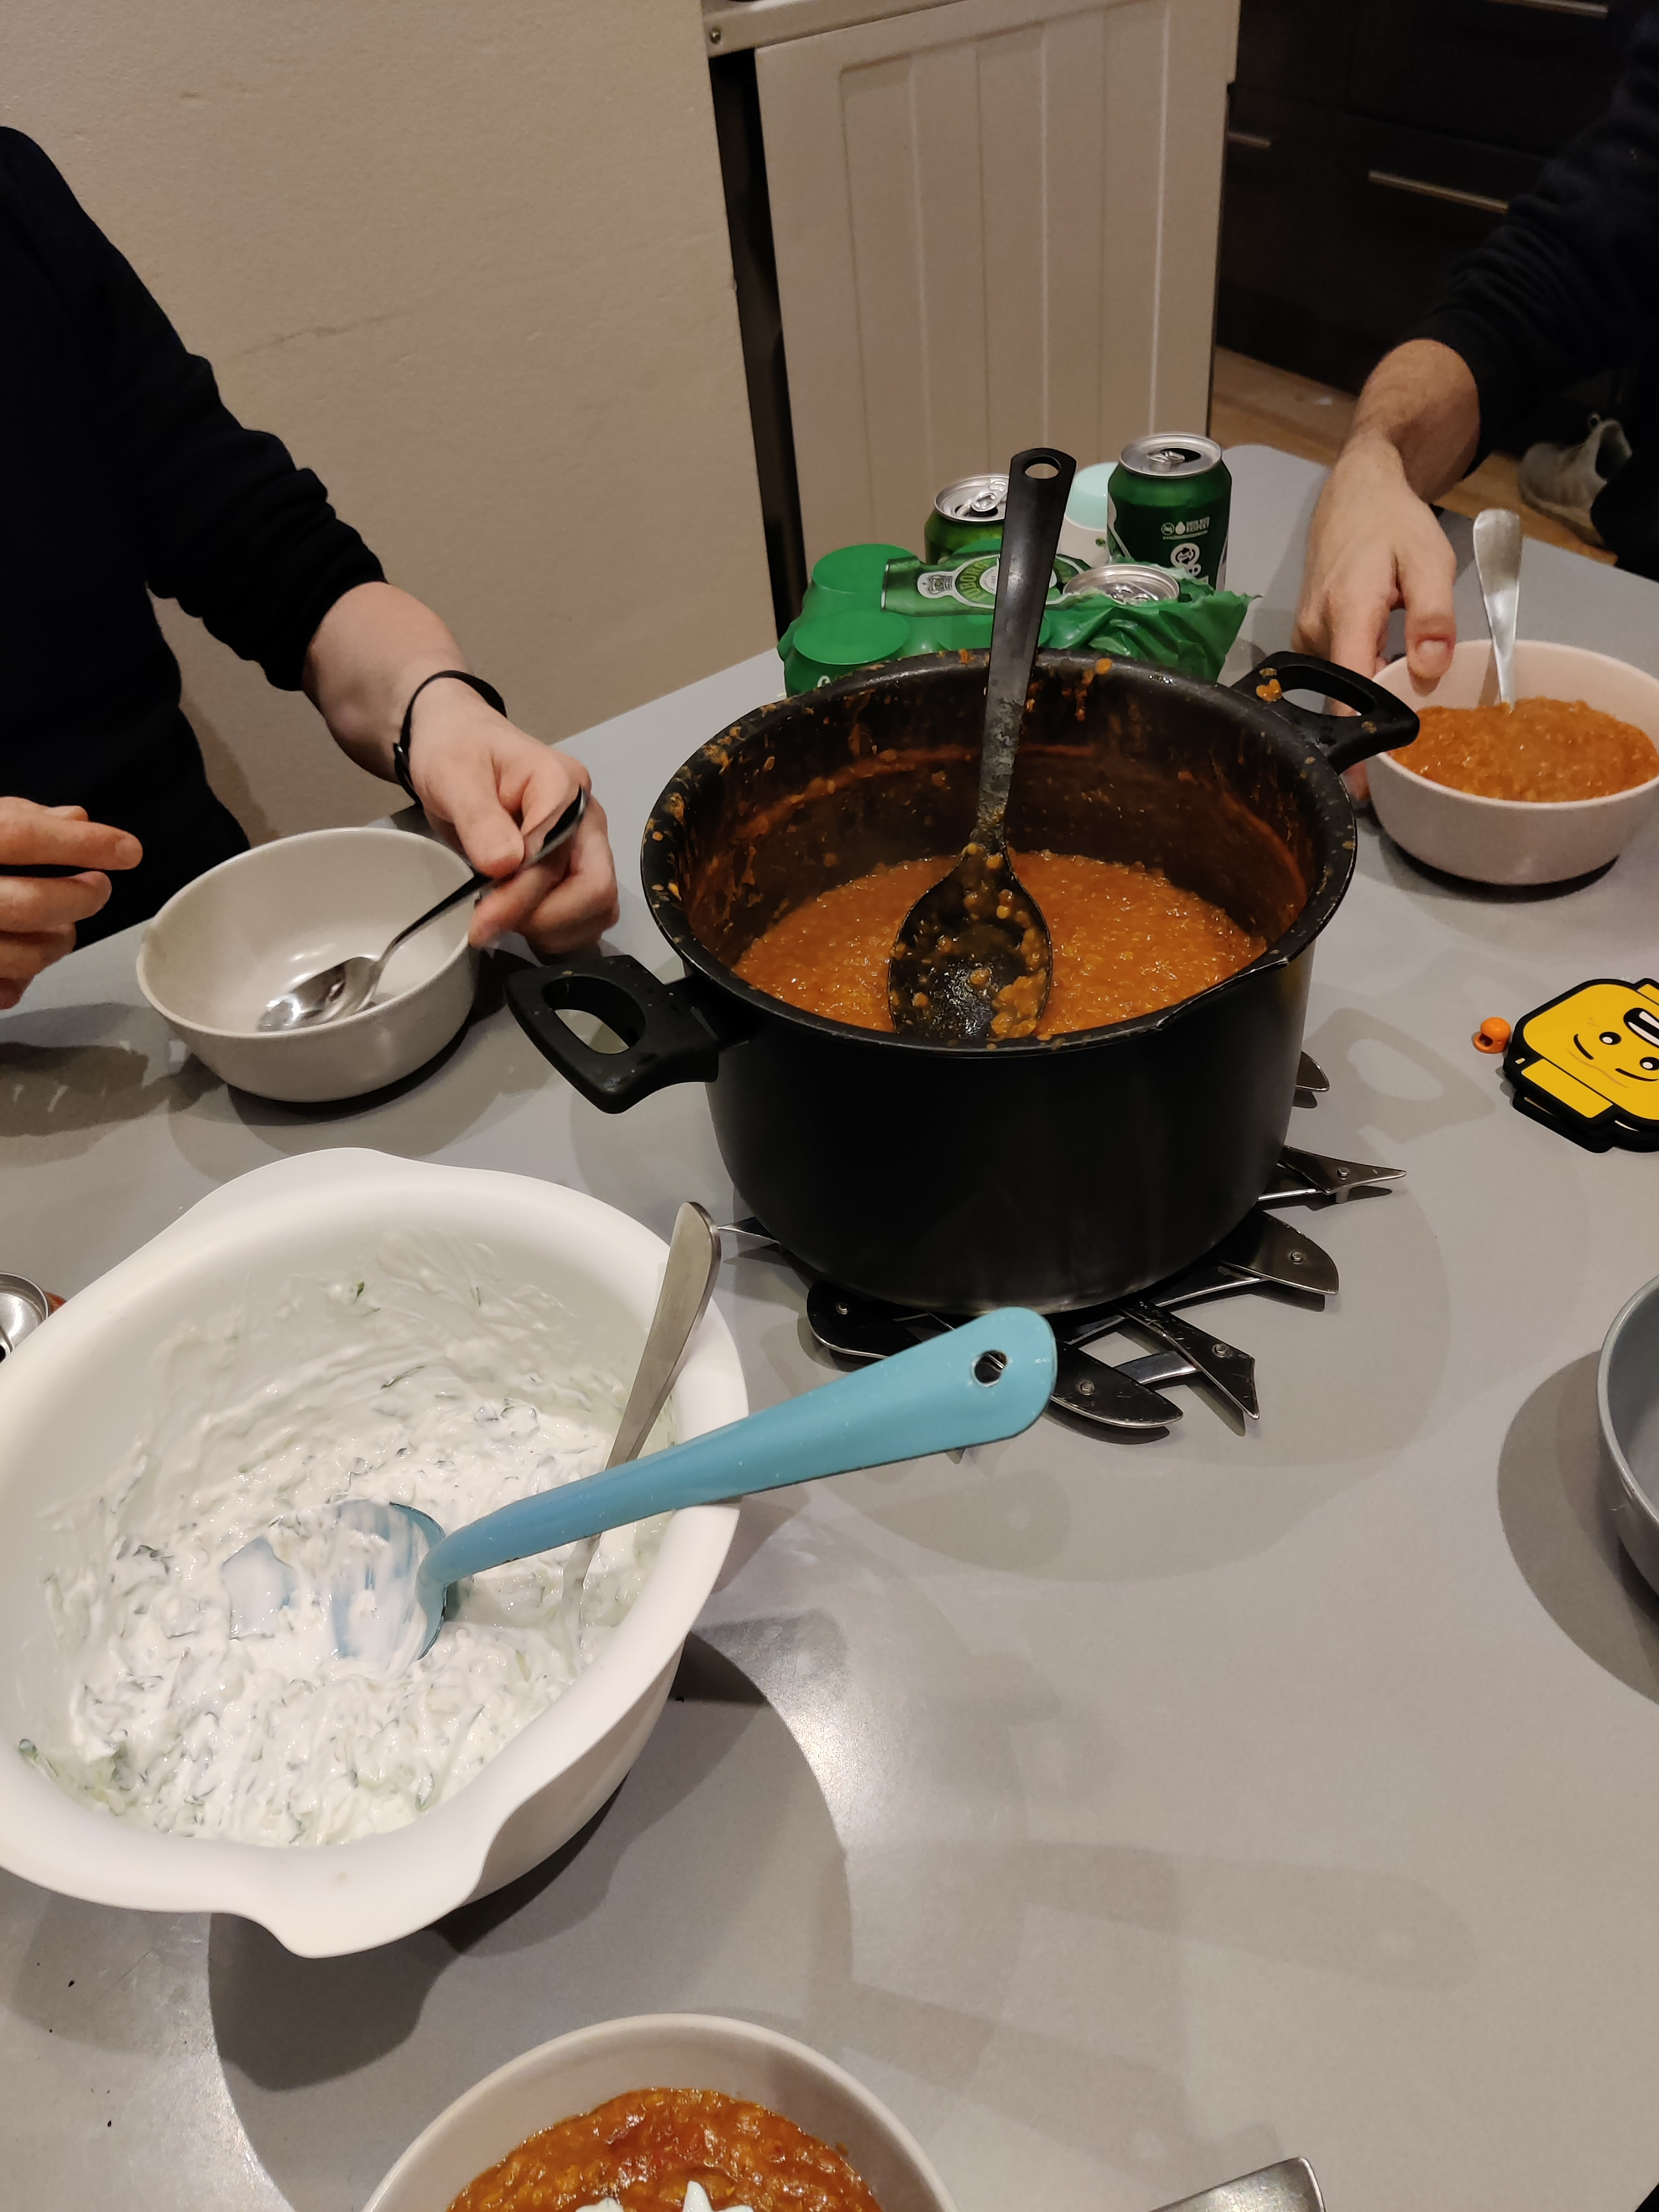
\includegraphics[width=\paperwidth,height=\paperheight]{Billeder/Aftensmad/Dahl.jpg}
    };
\end{tikzpicture}
\newpage \section{Kartoffel porre suppe}
\begin{minipage}[t]{0.5\textwidth}
\textbf{Ingredienser:}
\begin{itemize}
    \item 500g kartofler
    \item 3 porrer, skåret i ringe
    \item 1 løg, finthakket
    \item 20 g smør
    \item 3/4 L grøntsagsbouillon
    \item 1 dL piskefløde
    \item salt og peber
\end{itemize}
\textbf{Tilbehør og topping}
\begin{itemize}
    \item 150g bacon i tern
    \item Frisk timian
    \item Brød
\end{itemize}
\end{minipage}
\begin{minipage}[t]{0.5\textwidth}
\textbf{Fremgangsmåde:}
\begin{enumerate}
    \item Smelt smørret og svits kartofler, løg og porrer i 2-3 minutter
    \item Tilsæt grøntsagsbouillon, og lad koge i omtrent 15 minutter, til kartoflerne er møre.
    \item Blend kartoflerne i stykker med stavblender
    \item Tilsæt piskefløde og kog op, smag til med salt og peber
\end{enumerate}
\end{minipage}
\newpage Her mangler jeg sgu igen et billede, så her er et billede af mig i en kænguru 
\begin{figure}
    \centering
    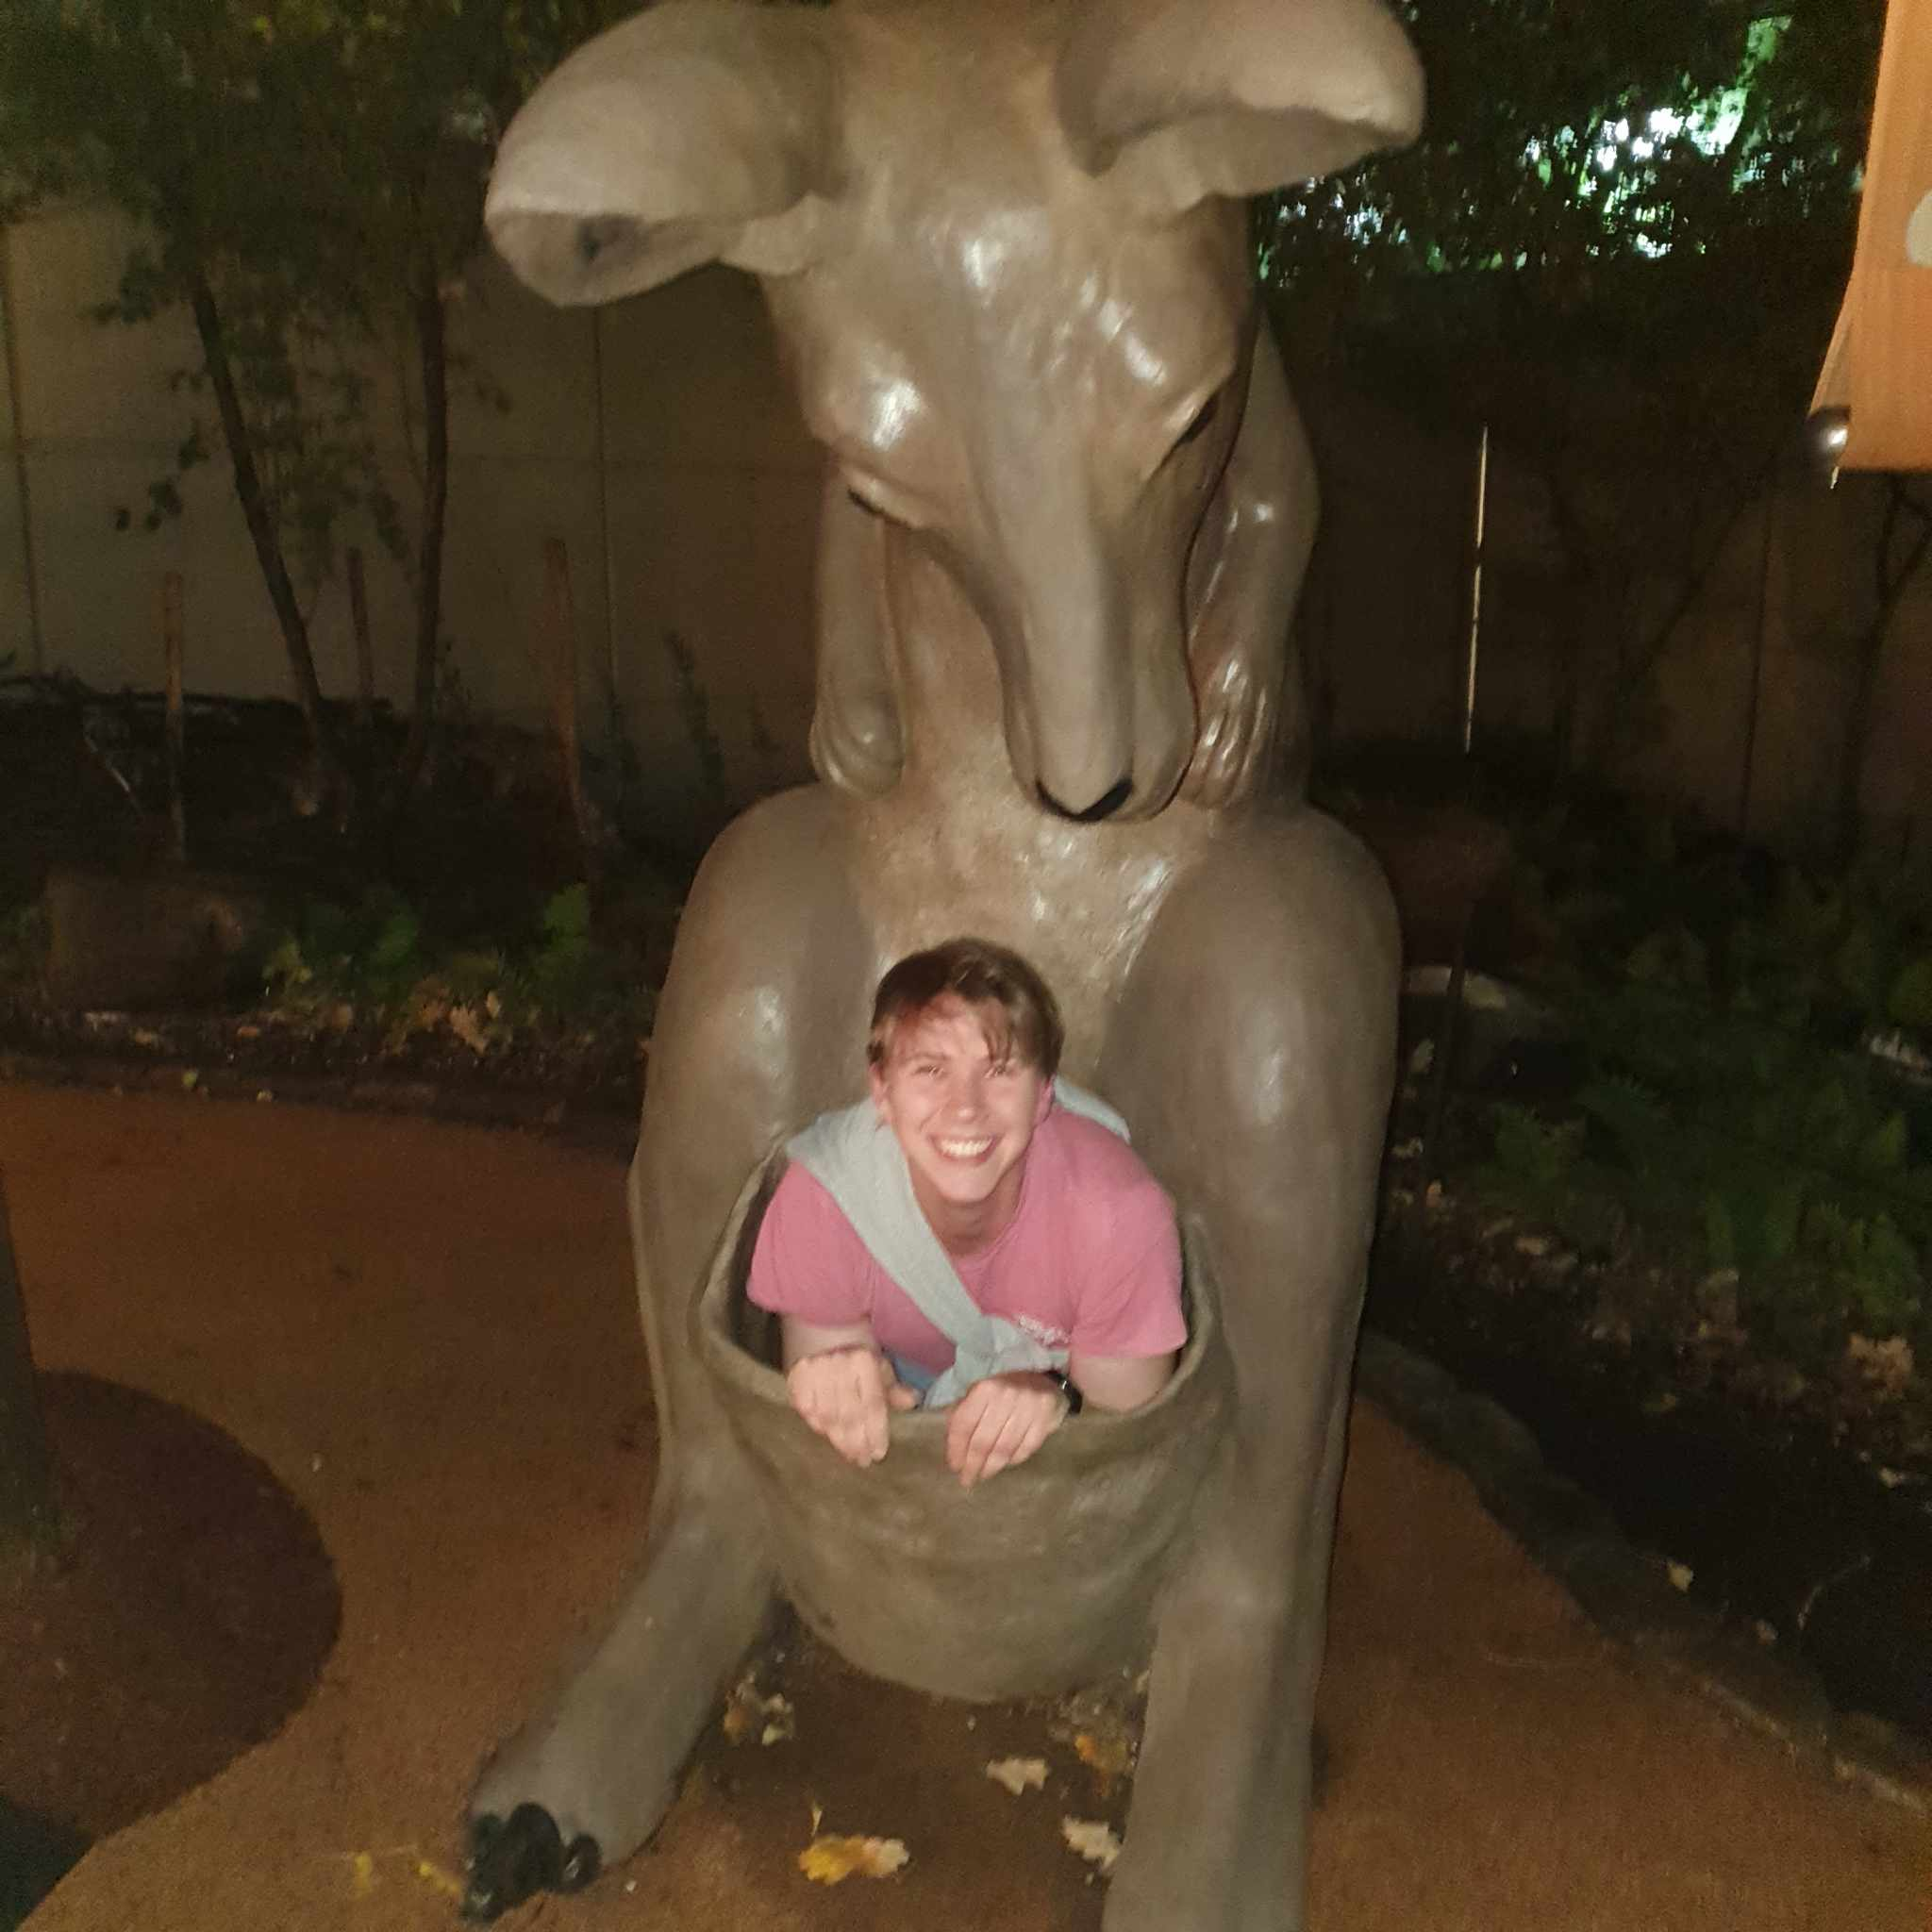
\includegraphics[width=0.5\linewidth]{Kenguru.jpeg}
    \caption{Kulturnat i 2023}
    
\end{figure}
\newpage \section{Løgsuppe}
\begin{minipage}[t]{0.5\textwidth}
\textbf{Ingredienser}
\begin{itemize}
    \item 500 g løg 
    \item 4-6 fed hvidløg
    \item timian
    \item salt og peber
    \item 1 L grøntsagsbouillon
    \item Eventuelt krydderi
    \begin{enumerate}
        \item Chiliflager
        \item Cayennepeber
        \item Rosmarin
    \end{enumerate}
\end{itemize}
\end{minipage}
\begin{minipage}[t]{0.5\textwidth}
\textbf{Fremgangsmåde:}
\begin{enumerate}
    \item Svits løgene til gyldne og tilsæt krydderier
    \item Tilsæt dernæst grøntsagsbouillon og kog op
    \item Lad simre i mindst 20 minutter
\end{enumerate}
\end{minipage}
Hvis man smider løgene i en foodprocessor, bliver suppen en anelse flydende, men smagen er der stadigvæk.
\newpage 
Her har jeg så igen glemt at tage et billede, så i stedet for mig der spiser løgsuppe, er der mig som drikker mad på fad i mBAR.
\begin{figure}
    \centering
    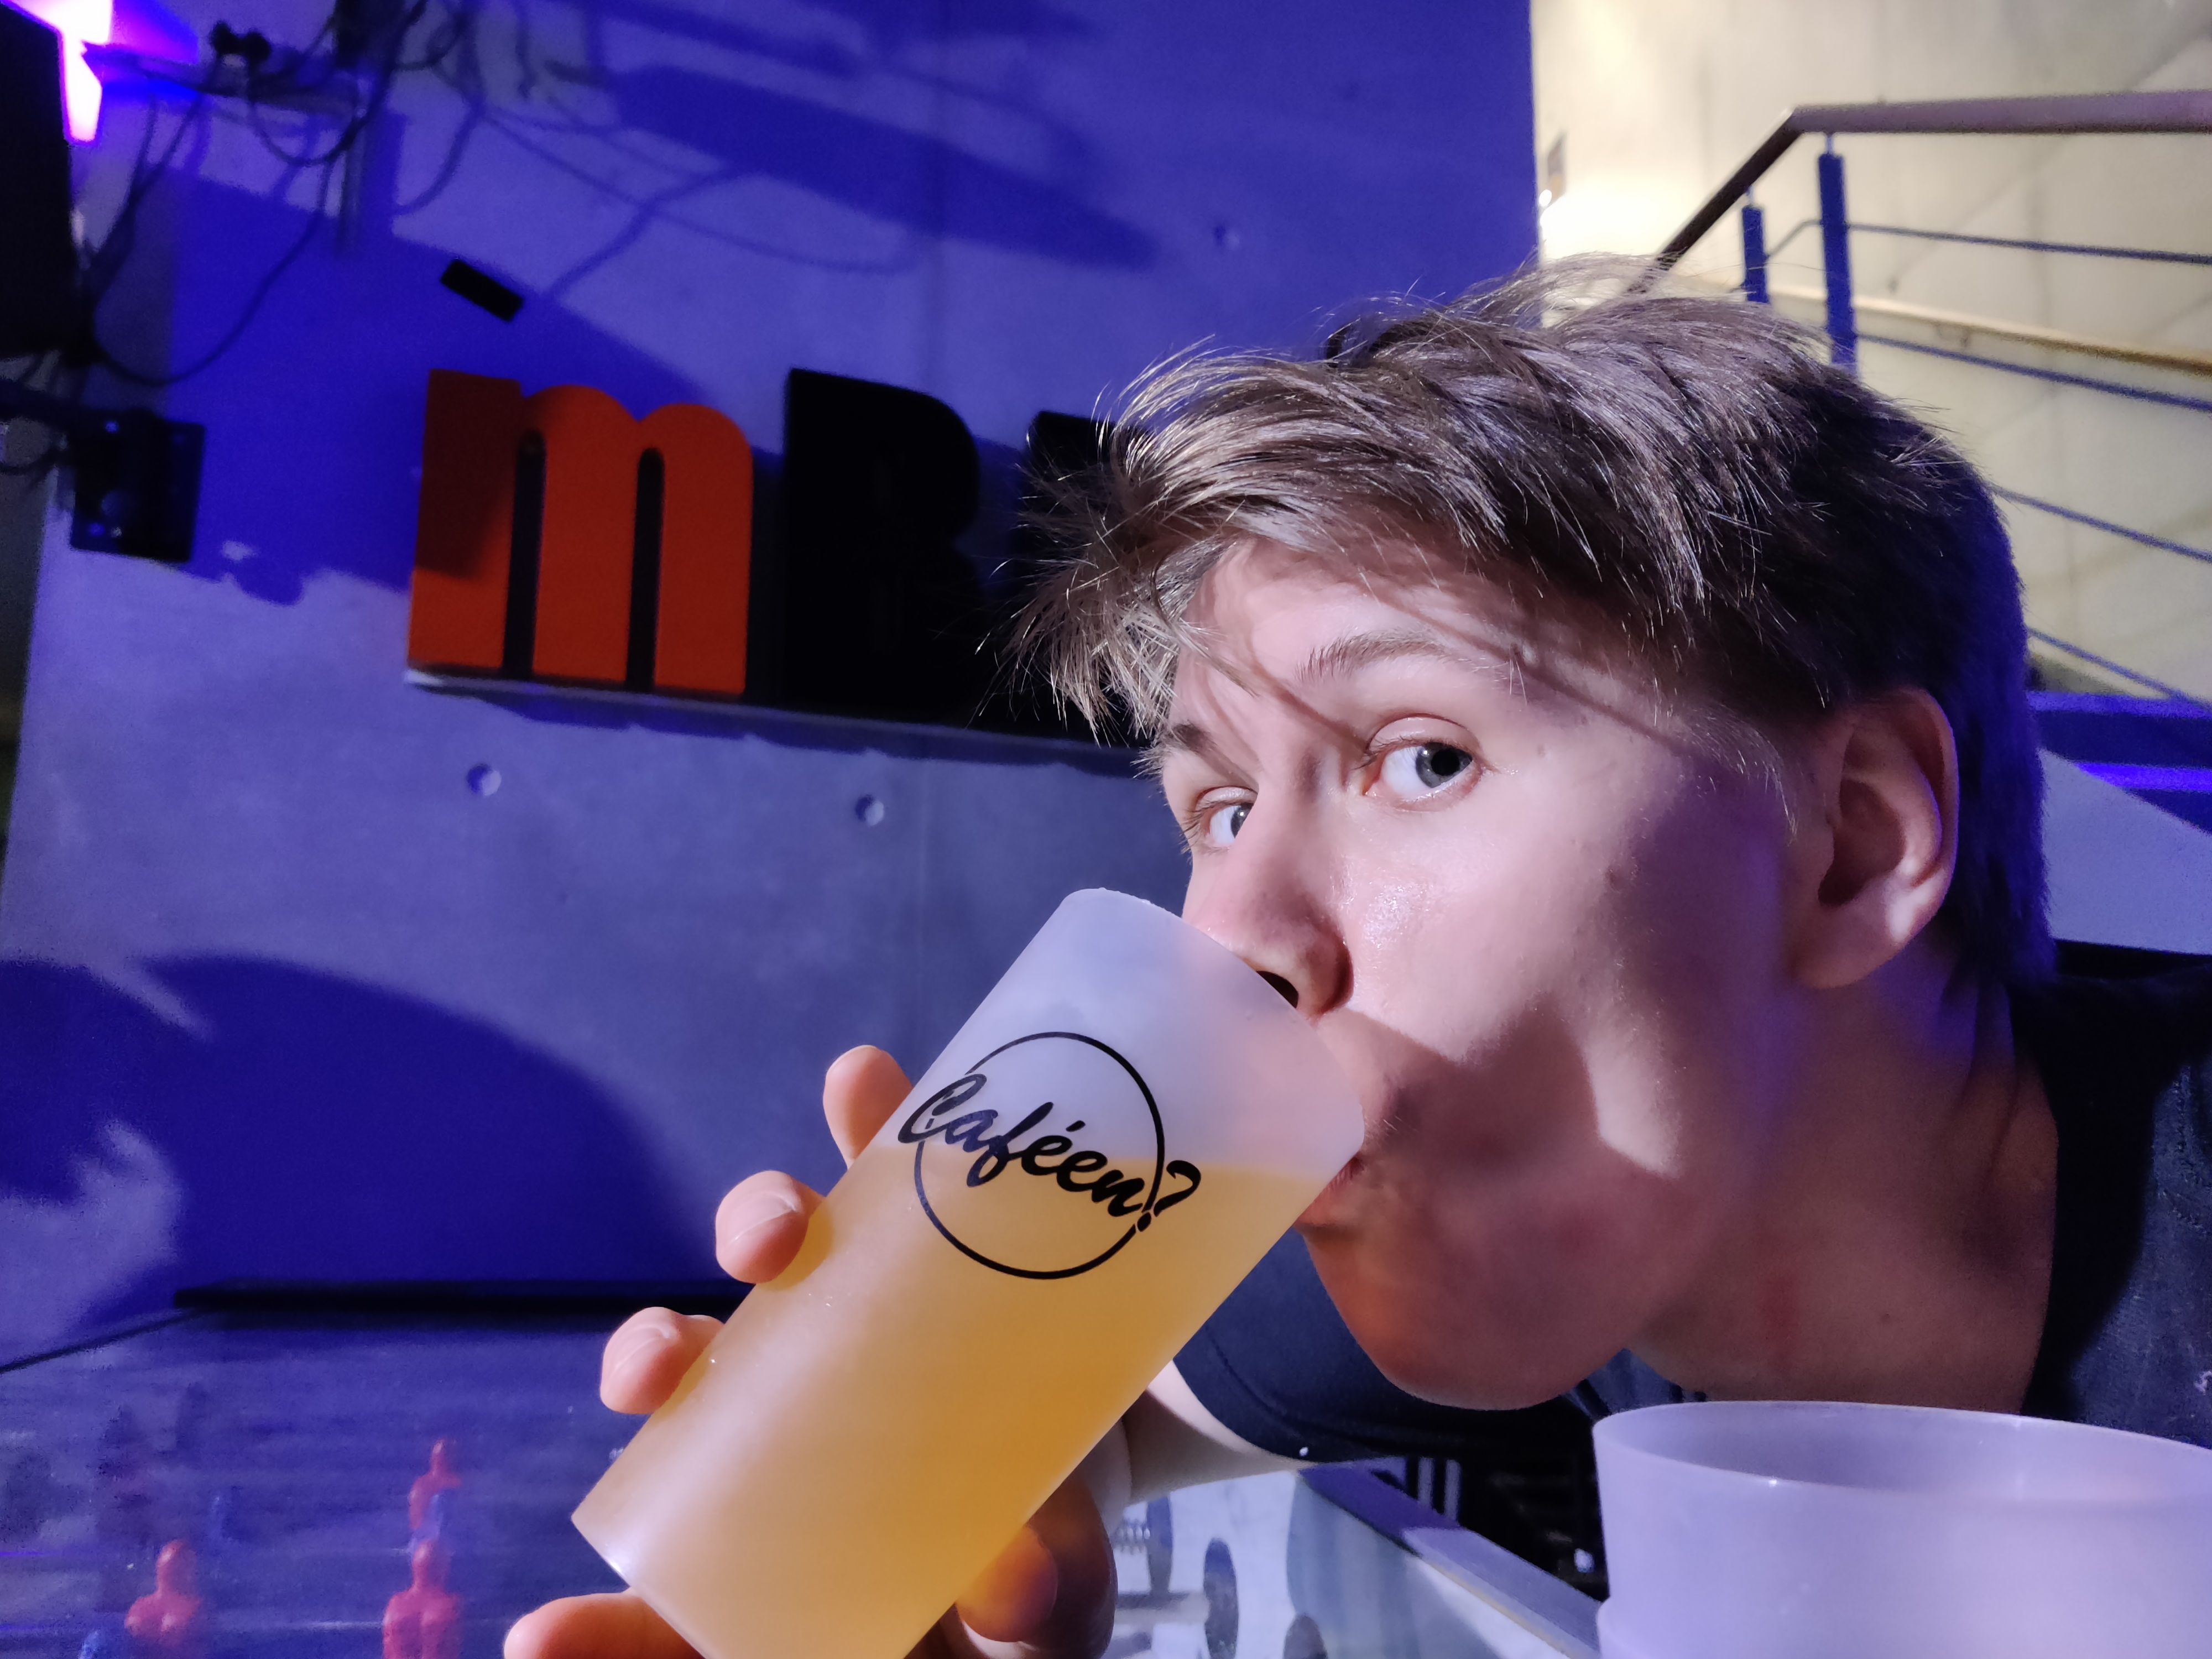
\includegraphics[width=0.5\linewidth]{mBAR.jpg}
    \caption{Mig i mBAR}
    
\end{figure}
\newpage 
\section{Ovnbagt aubergine}
\begin{minipage}[t]{0.5\textwidth}
\begin{itemize}
    \item 1 aubergine
    \item 10 g smør
    \item 1 fed hvidløg
    \item frisk timian
    \item salt og peber
\end{itemize}
\end{minipage}
\begin{minipage}[t]{0.5\textwidth}
\textbf{Fremgangsmåde:}
\begin{enumerate}
    \item Skær auberginen over på midten (oppe fra ned), og scoop \~ 1 skefuld aubergine kød ud.
    \item Rids fordybningen minimalt så smagen kan synke ind.
    \item Pak dem ind i sølvpapir og smid i ovnen på 200 \degree C varmluft i 15 minutter
    \item Når auberginerne er færdige skal de gerne være let brunet, og halvsprøde i overfladen.
\end{enumerate}
\end{minipage}
Det er let at opskalere opskrift til flere aubergine, det vigtigste er at auberginerne er af nogenlunde størrelse. Hvidløget kan enten presses og dermed blive i, eller mases til større stykker så saften blandet sig med smørret.
\newpage 
Fremfor et billede af en lækker aubergine, kommer der i stedet for et billede fra Biokemi galla 2023
\begin{figure}
    \centering
    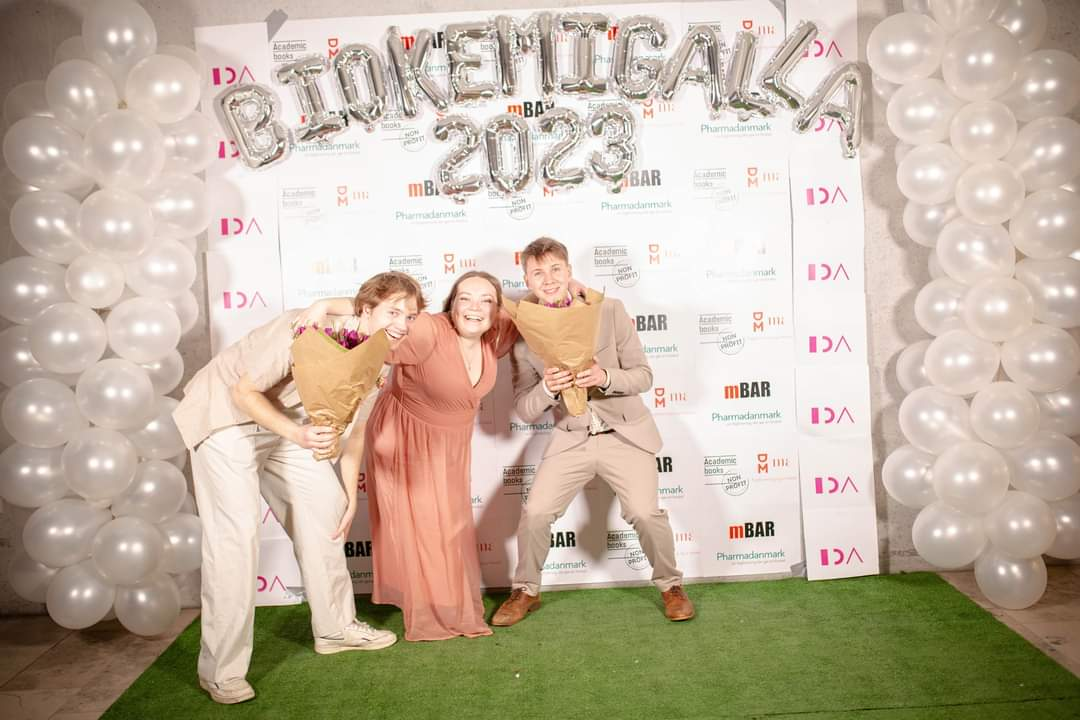
\includegraphics[width=0.5\linewidth]{Galla.jpg}
    \caption{Billedet fra biokemigalla 2023}
\end{figure}
\newpage \section{Ovnbagte søde kartofler}
Til retten anbefaler jeg søde kartofler cirka på størrelse med bagekartofler, da dette giver en bedre mulighed for at fylde den ud. Retten skal lidt ses som en sødekartoffelmos, som der stadig er i dens skræld. Man kan med fordel tilføje flere grøntsager som fyld, men dette er min umiddelbare anbefaling\\
\begin{minipage}[t]{0.5\textwidth}
\textbf{Ingredienser:}
\begin{itemize}
    \item 2-3 Søde kartofler
    \item Smeltet smør
    \item Hvidløg
\end{itemize}
\underline{Fyldet:}
\begin{itemize}
    \item Avokado 
    \item Pico de Gallo
    \item Bønnepasta
    \item Græsk yoghurt dressing 
\end{itemize}
\end{minipage}
\begin{minipage}[t]{0.5\textwidth}
\begin{enumerate}
    \item Skær ridser i de søde kartofler og således at smørret og hvidløget kan sive ned i.
    \item Bag i ovnen i omtrent 1 time ved 180 C°, til blød i midten.
    \item Mos kartoflen delvis og bland fyldet ned i kartoflen, jeg bleger at genopfylde løbende.  
\end{enumerate}
\end{minipage}
\newpage
\begin{tikzpicture}[remember picture,overlay,inner sep=0pt,outer sep=0pt]
    \node[anchor=south east] at (current page.south east) {
        \includegraphics[width=\paperwidth,height=\paperheight]{Billeder/Aftensmad/Ovnbagt_sødkartoffel.jpg}
    };
\end{tikzpicture}
\newpage \section{Ratatoulie}
\begin{minipage}[t]{0.5\textwidth}
\textbf{Ingredienser:}
\\ Til Sovsen:
\\ Til sovsen kan man passende bruge min opskrift på arabiatta (det plejer jeg hvert fald)
\begin{itemize}
    \item 1 dåse flåede tomater
    \item 3 spsk olivenolie
    \item 1 tsk balsamico
    \item 1 tsk sukker
    \item Citronsaft
    \item 1-2 håndfuld basilikum
    \item 1/2 tsk chiliflager 
    \item 2-3 presset fed hvidløg
    \item 1 finthakket løg
\end{itemize}
Til Toppen:
\begin{itemize}
    \item Tomater
    \item Aubergine
    \item Squash 
\end{itemize}
Dressing:
\begin{itemize}
    \item Olivenolie
    \item Frisk Timian
\end{itemize}
\end{minipage}
\begin{minipage}[t]{0.5\textwidth}
\textbf{Fremgangsmåde:}
    \begin{enumerate}
        \item Hæld tomatsovsen i et fad (omtrent 3-4 centimeter)
        \item Skær grøntsagerne ud i skiver, ikke for tynde.
        \item Arranger skiverne i mønster oven på tomatsovsen i fadet.
        \item Drys olivenoliedressingen oven på
   \end{enumerate}

\end{minipage}
Til ratatouillen er det vigtigt at vælge gode grøntsager til toppen. Jeg er personlig fan af de 3 overstående men man kan sagtens vælge andet, jeg vil dog fraråde at bruge, butternut squash og andre former for græskar da de ikke får den ønskede konsistens. Jeg har endnu ikke fået det til at ligne ratatouille som set i dokumentarfilmen Ratatouille 
\newpage
\begin{tikzpicture}[remember picture,overlay,inner sep=0pt,outer sep=0pt]
    \node[anchor=south east] at (current page.south east) {
        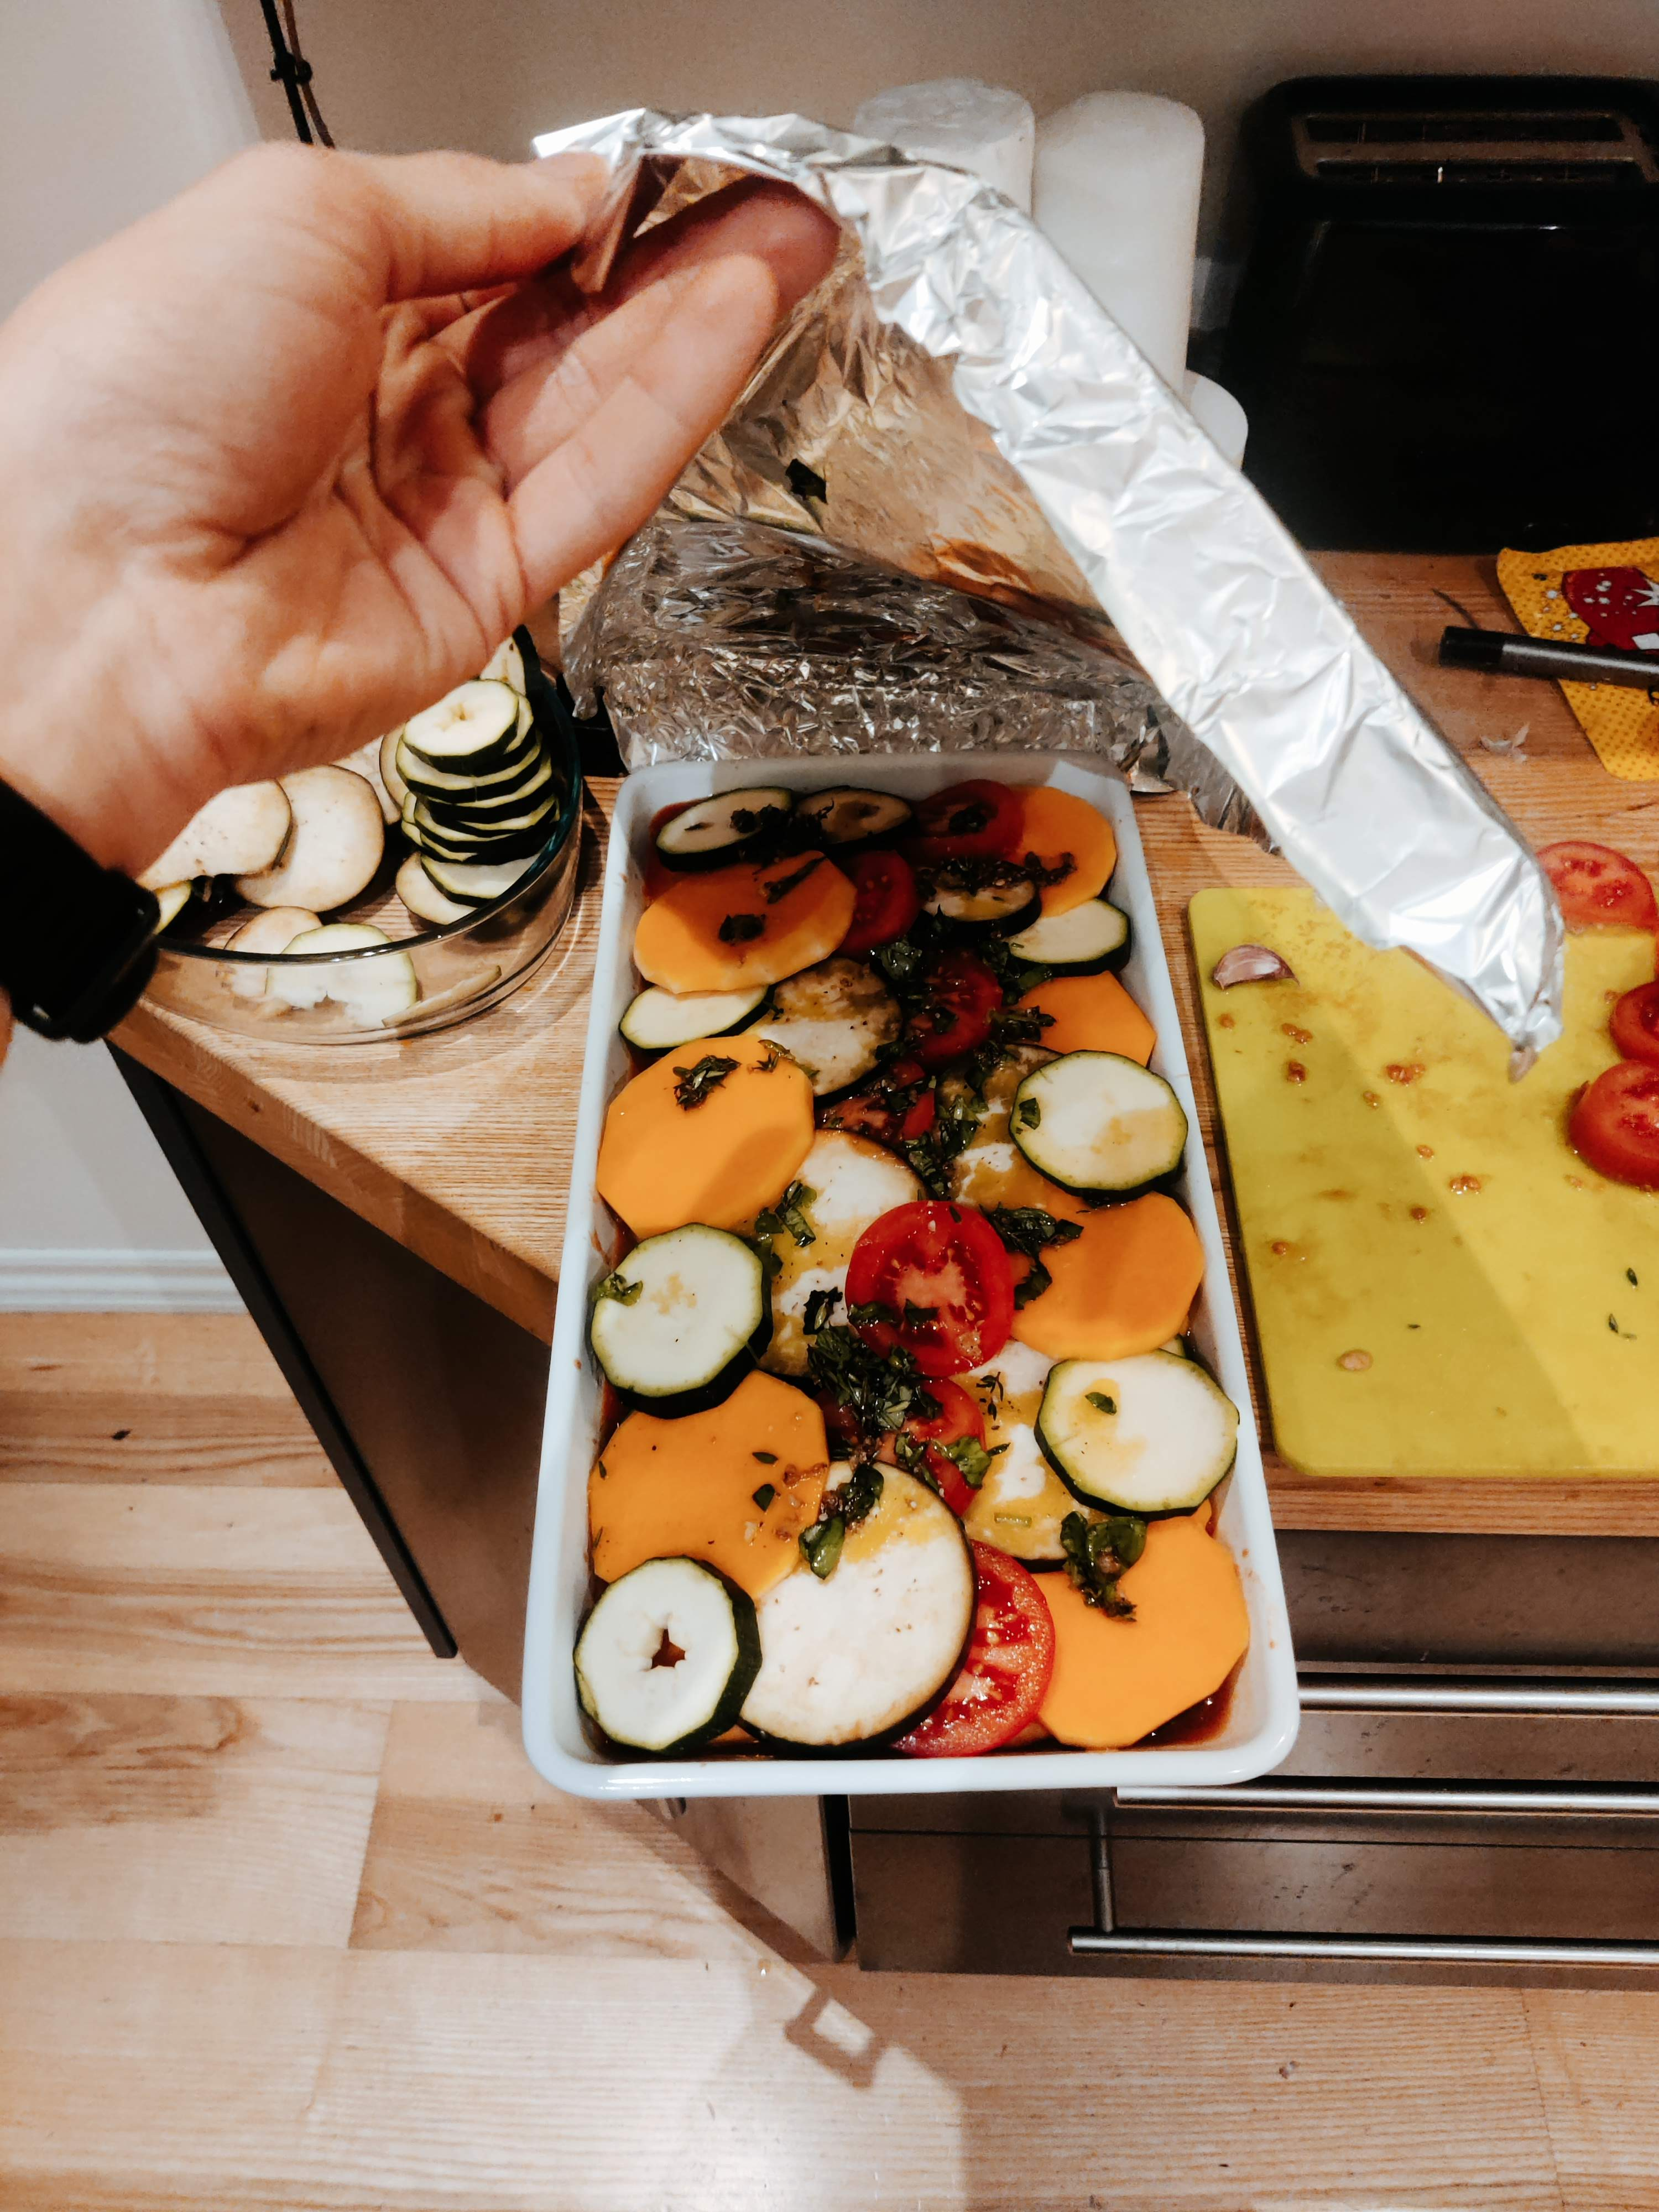
\includegraphics[width=\paperwidth,height=\paperheight]{Billeder/Aftensmad/Ratatoulie.jpg}
    };
\end{tikzpicture}
\newpage 
\section{Risotto Svampe}
\begin{minipage}[t]{0.5\textwidth}
\textbf{Ingredienser:}
\begin{itemize}
    \item 1 løg, finthakket
    \item 1 fed hvidløg, finthakket
    \item 400 g risotto ris
    \item 300 g champignon
    \item 1 L grøntsagsbouillon
    \item 50 g parmesan, friskrevet
    \item 1 dL piskefløde
    \item 20 g smør
    \item 1 kop hvidvin
\end{itemize}
\end{minipage}
\begin{minipage}[t]{0.5\textwidth}
\textbf{Fremgangsmåde:}
\begin{enumerate}
    \item Svits løgene og hvidløgene til gyldne.
    \item Tilsæt risottorisen, vin og 300 mL grøntsagsbouillon.
    \item Tilsæt resten af grøntsagsbouillonen lidt efter lidt, til risene er møre (ca. 20 minutter).
    \item Vend osten og fløden i, og lad osten smelte under konstant omrøring.
\end{enumerate}
\end{minipage}
\newpage  \newpage \begin{tikzpicture}[remember picture,overlay,inner sep=0pt,outer sep=0pt]
    \node[anchor=south east] at (current page.south east) {
        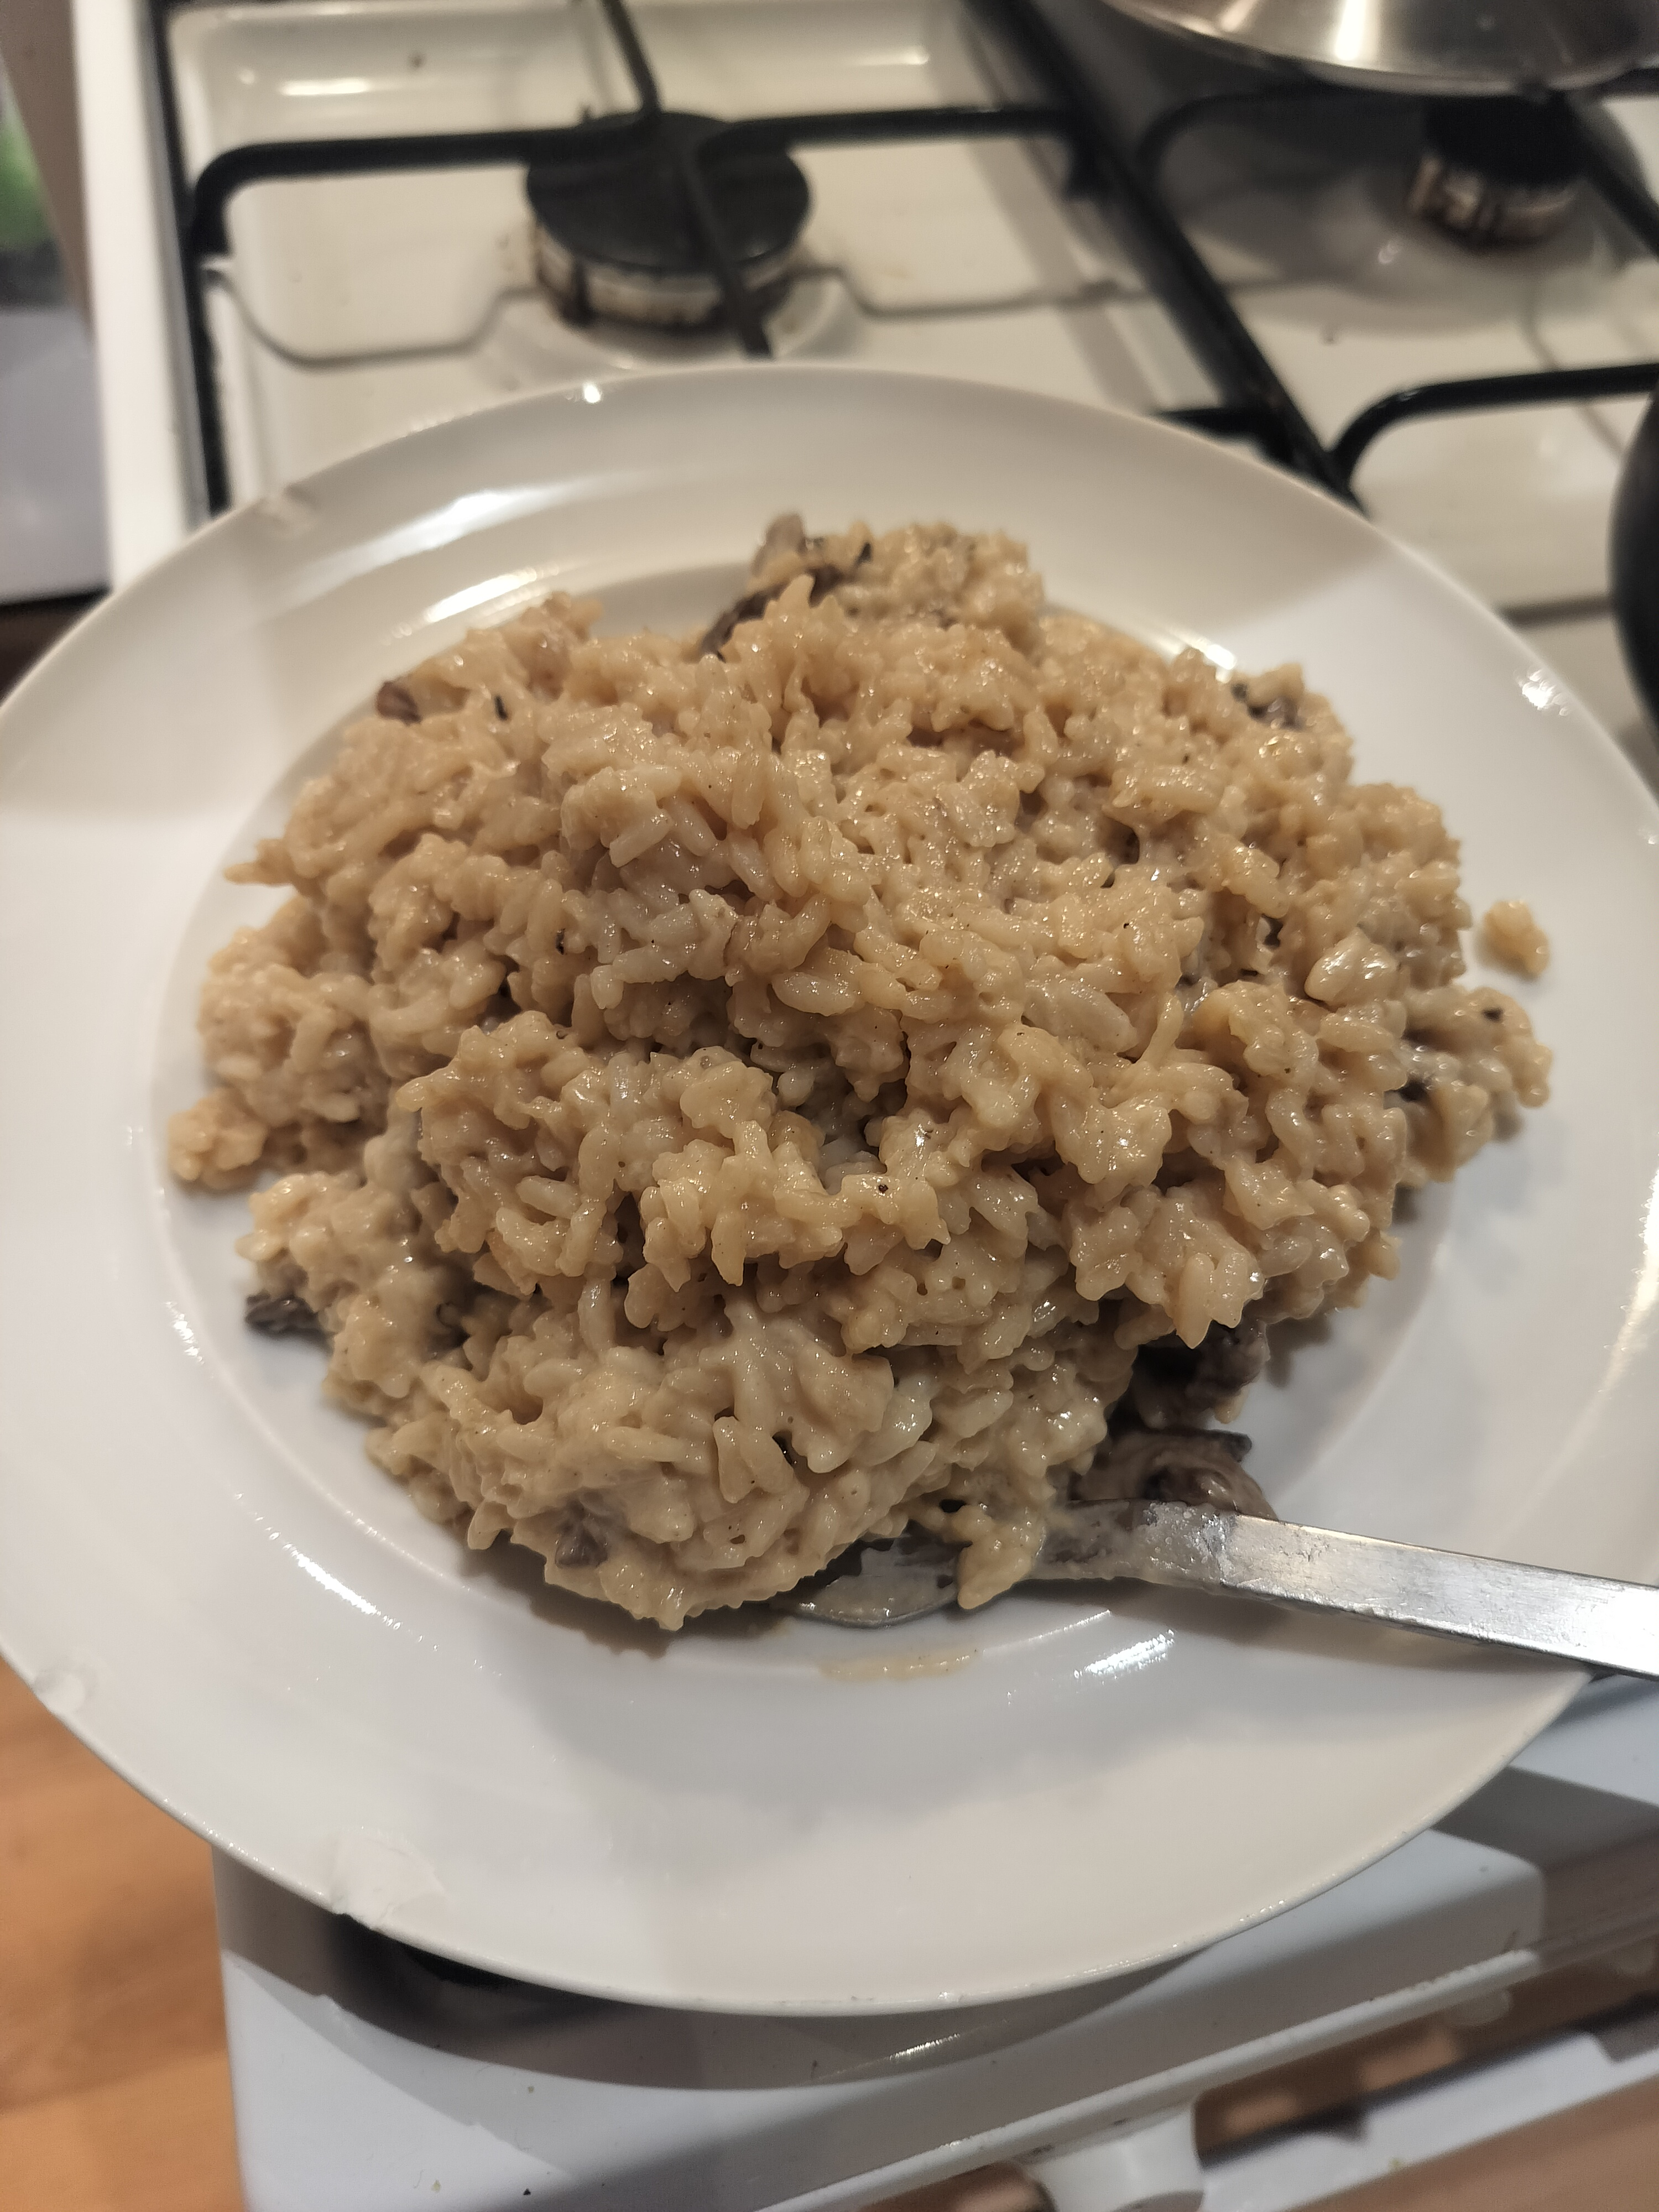
\includegraphics[width=\paperwidth,height=\paperheight]{Billeder/Aftensmad/Risotto.jpg}
    };
\end{tikzpicture}

%Her skulle der helst også være et billede, men i stedet for tager vi et billede af mig på ski i Italien
%\begin{figure}
%    \centering
%   \includegraphics[width=0.5\linewidth]{Ski.jpg}
%    \caption{Ski tur i Italien}
%\end{figure}
\newpage \section{Risotto Pasta}
\begin{minipage}[t]{0.5\textwidth}
\textbf{Ingredienser}
\begin{itemize}
    \item 2 løg, finthakket
    \item 3 fed hvidløg, presset
    \item 2 spsk olivenolie
    \item 1 grøntsagsbouillonterning
    \item svampe
    \begin{itemize}
        \item 250 g champignoner 
        \item 100 g Portobello svampe (kan undlades)
        \item 50g kantareller (kan undlades)
    \end{itemize}
    \item 50g parmassen
    \item 2.5 dL fløde
    \item 250g frisk pasta
    \item Krydderier
    \begin{itemize}
        \item 1 tsk timian
        \item kantarelfond
        \item salt og peber
    \end{itemize}
\end{itemize}
\end{minipage}
\begin{minipage}[t]{0.5\textwidth}
\textbf{Fremgangsmåde:}
\begin{enumerate}
    \item Svits løgene i olie.
    \item Tilsæt de hakkede svampe, og steg til bløde.
    \item Tilsæt den friske pasta, bouillonterningen, og vand nok til at dække pastaen.
    \item Når pastaen har fået den rette konsistens, skal noget af vandet hældes fra, og fløden og osten tilsættes.
\end{enumerate}
\end{minipage}
Til denne opskrift er det vigtigste at man har svampe i, kantareller tilføje en hel masse lækker smag, men er ikke altid så let at få fat i, overordnet set vil jeg putte flere svampe i end men umiddelbart skulle tro, men elsker også svampe.
\newpage \begin{tikzpicture}[remember picture,overlay,inner sep=0pt,outer sep=0pt]
    \node[anchor=south east] at (current page.south east) {
        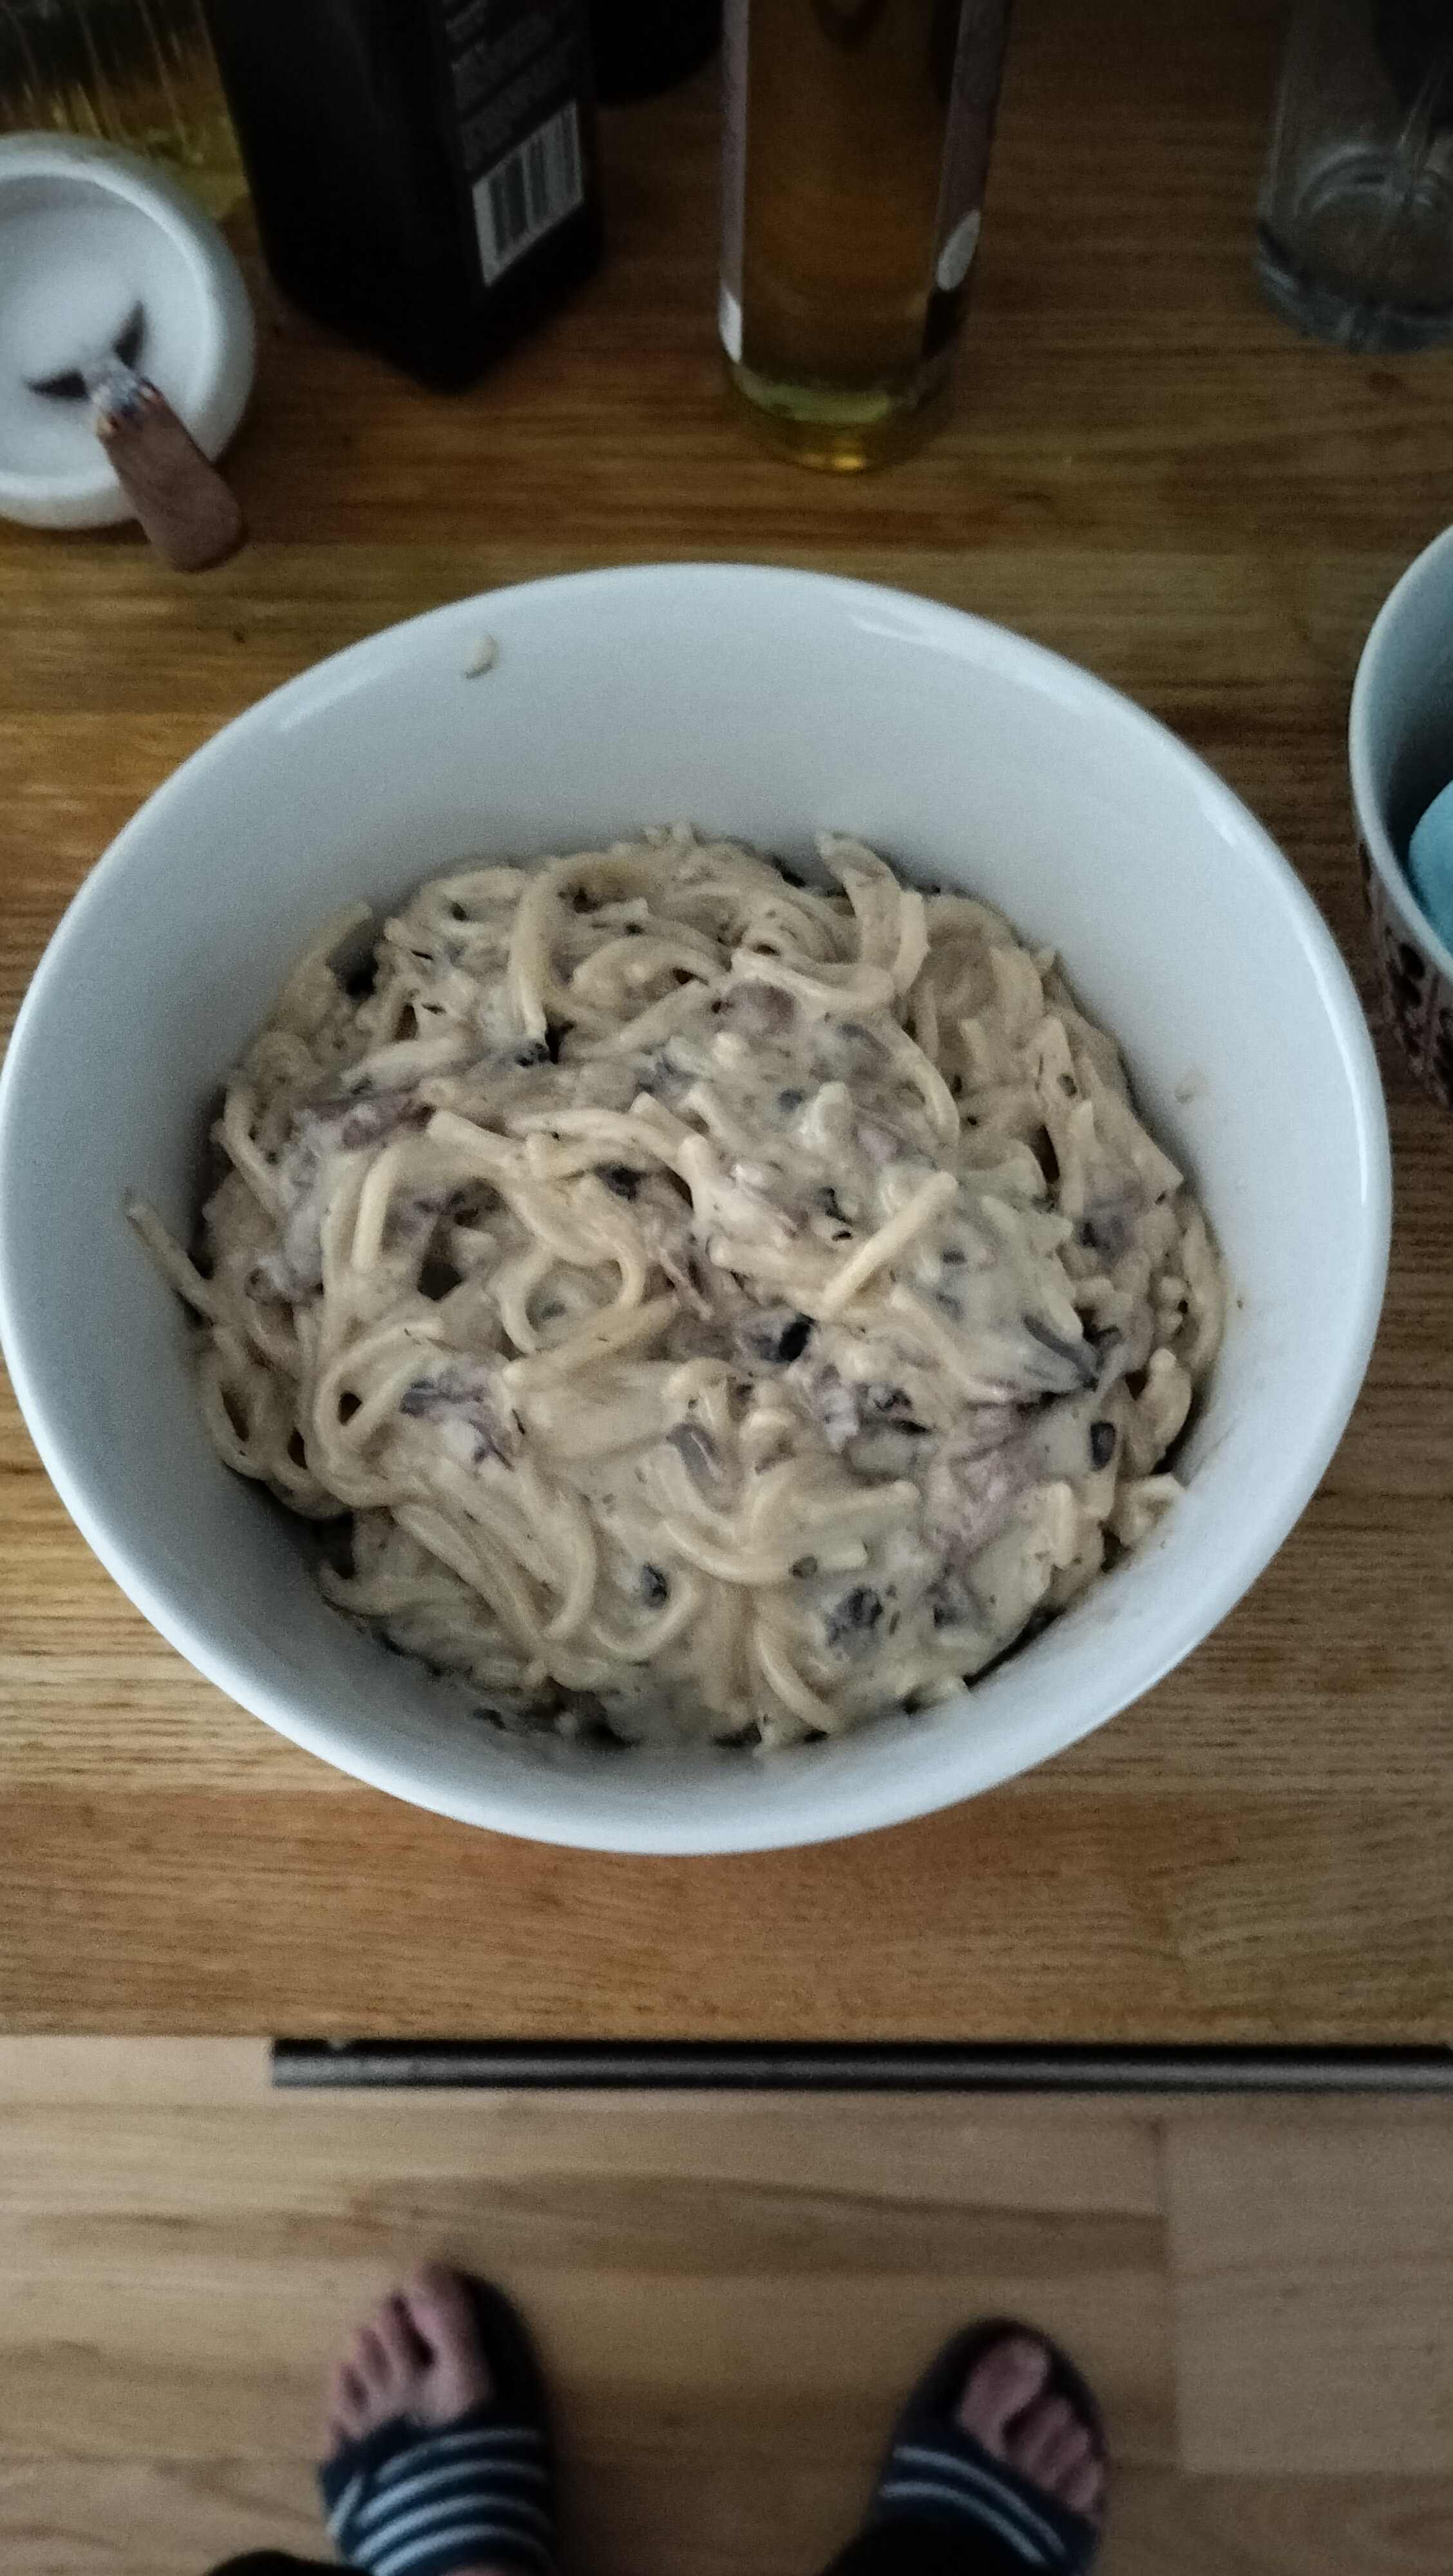
\includegraphics[width=\paperwidth,height=\paperheight]{Billeder/Aftensmad/PAstotto.jpg}
    };
\end{tikzpicture}
\newpage \section{Timian Kartofler}
\begin{minipage}[t]{0.5\textwidth}
\textbf{Ingredienser:}
\begin{itemize}
    \item 500 g kartofler, skåret i både
    \item 3 spsk olivenolie
    \item Timian
    \item Salt og peber
    \end{itemize}
\end{minipage}
\begin{minipage}[t]{0.5\textwidth}
\textbf{Fremgangsmåde:}
\begin{enumerate}
    \item Skyld kartoflerne, og skær dem i både (cirka i 1/4 på langs).
    \item Anbring i ovnfast fad, og tildæk med olivenolie og timian.
    \item Bag ved 200 \degree C varmluft i 40 minutter, sørg for at vende dem et par gange undervejs.
\end{enumerate}
\end{minipage}
Bagetiden af timiankartoflerne kommer and på hvor tykke kartoflerne er skåret, hvis det er meget tynde både, skal de have mindre i ovnen. Jeg anbefaler at man tester "færdigheden" ved at stikke dem med en gaffel, hvor de skal være bløde inden i, og brune uden på.
\\
\underline{Samlet tid: 1 time}
\newpage Her skulle der også have været et billedet, i stedet for kommer der et billede af mit kostume til min 23 års fødselsdag 
\begin{figure}
    \centering
    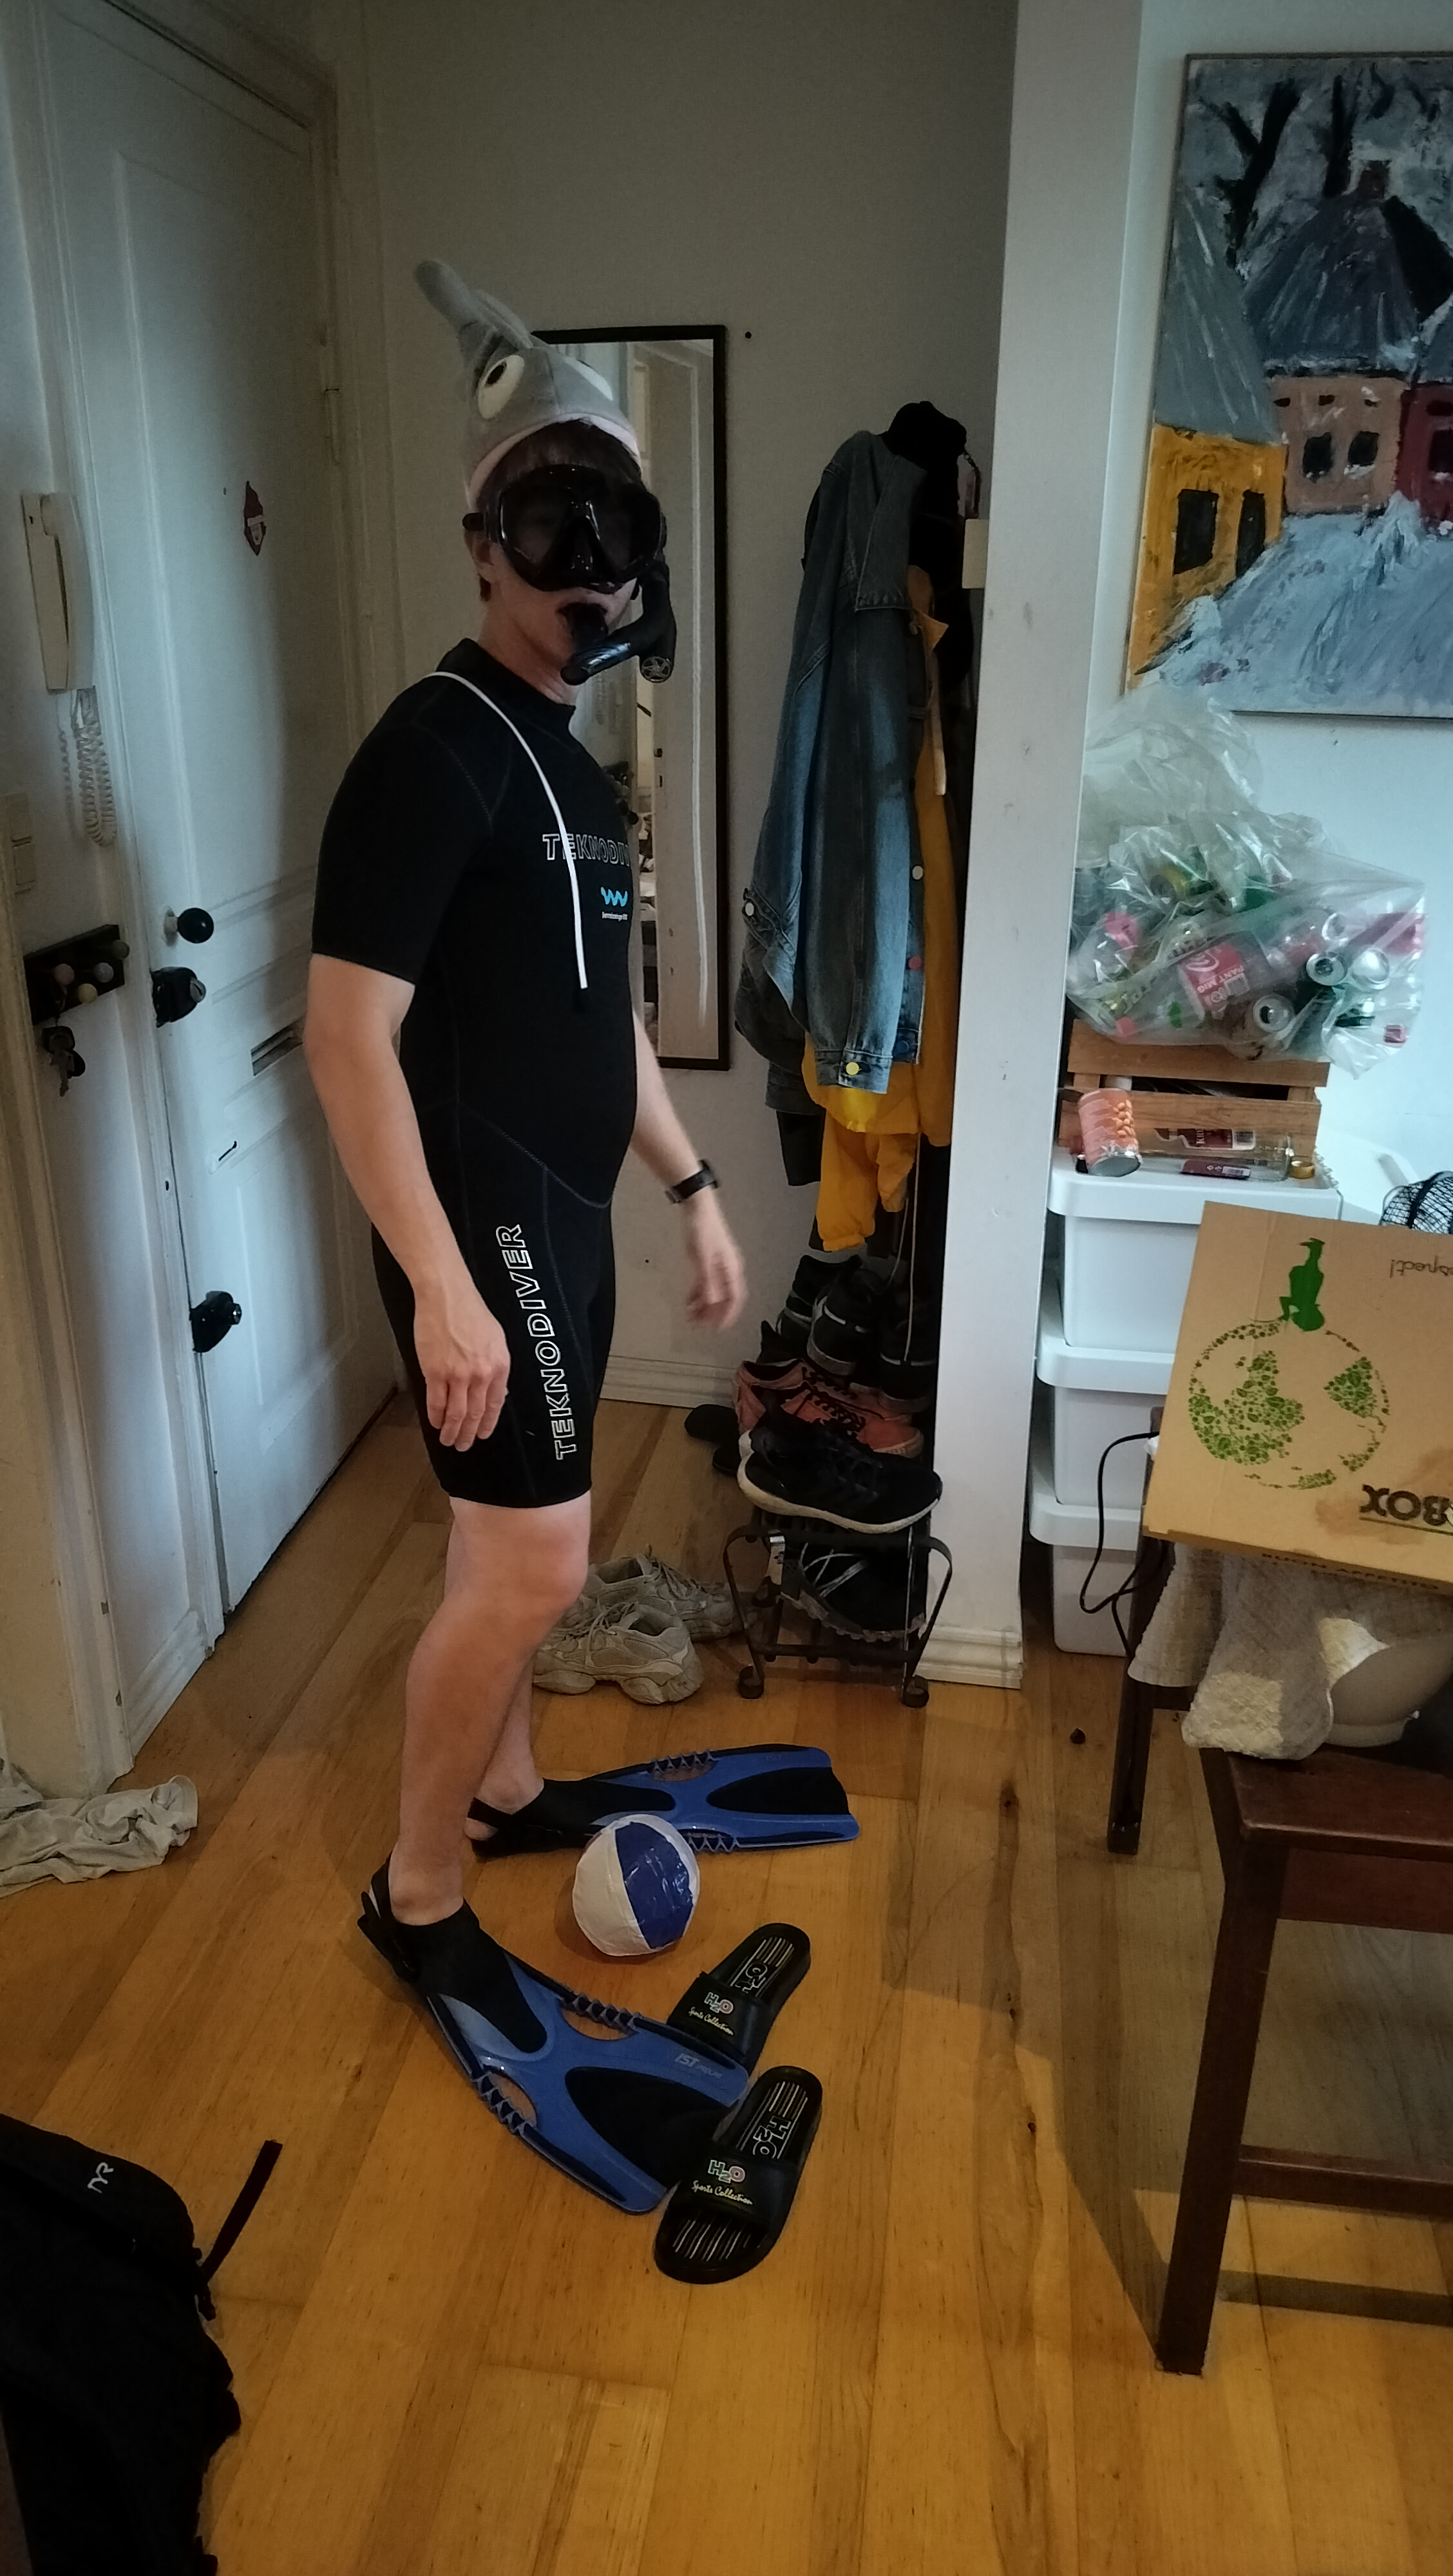
\includegraphics[width=0.5\linewidth]{Dykke.jpg}
    \caption{Dykker der brutalt bliver spist af en haj}   
\end{figure}
\newpage \section{Udon Nudel Suppe}
\begin{minipage}[t]{0.5\textwidth}
\textbf{Ingredienser:}
\begin{enumerate}
    \item 200g udon nudler
    \item 2 æg, hårdkogte
    \item 1-2 forårsløg, skåret i ringe
    \item 75 g champignoner, skiveskåret 
    \item 50 g gulerødder, skiveskåret 
    \item 0.5 L grøntsagsbouillon 
    \item evt.
    \begin{itemize}
        \item Bønnespirer til topping
        \item Majs
        \item Ærter
        \item Mukimame bønner
    \end{itemize}
\end{enumerate}
\end{minipage}
\begin{minipage}[t]{0.5\textwidth}
\textbf{Fremgangsmåde:}
\begin{enumerate}
    \item Klargør ingredienserne.
    \item Kog udon nudlerne i grøntsagsbouillon, sammen med de skiveskårede gulerødder.
    \item Pil æggene og server i halve , oven på nudelsuppen sammen med forårsløgene, champignoner og de andet ønsket topping.  
\end{enumerate}
\end{minipage}
Opskriften kan let opskaleres, og dette er bare nogle forslag på hvilke grøntsagerne, der kunne være lækre i. Generelt vil jeg foreslå grøntsager som er "friske" i smagen, som også ses i eventuelt.
\newpage \begin{tikzpicture}[remember picture,overlay,inner sep=0pt,outer sep=0pt]
    \node[anchor=south east] at (current page.south east) {
        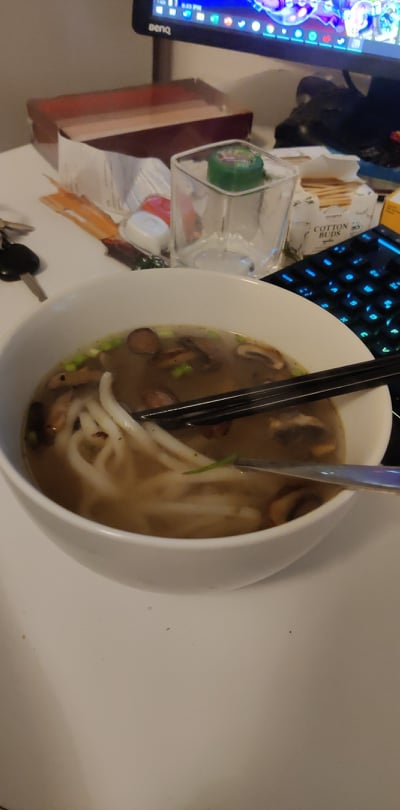
\includegraphics[width=\paperwidth,height=\paperheight]{Billeder/Aftensmad/Udon_nudel_Suppe.jpeg}
    };
\end{tikzpicture}
\chapter{Tilbehør}
\minitoc
\newpage \section{Bønnepasta}
\begin{minipage}[t]{0.5\textwidth}
\textbf{Ingredienser}
\begin{itemize}
    \item 2 mellemstore løg finthakket
    \item 1-2 fed hvidløg presset
    \item 1 dåse sorte bønner
    \item 1 tsk tomatpasta
    \item Evt. 1 dåse hakkede tomater
    \item krydderier
    \begin{itemize}
        \item 2 tsk Paprika
        \item 1 tsk Chiliflager
        \item 1 tsk Cayennepeber
        \item 0.5 tsk stødt spidskommen
        \item salt og peber
    \end{itemize}
\end{itemize}
\end{minipage}
\begin{minipage}[t]{0.5\textwidth}
\textbf{Fremgangsmåde:}
\begin{enumerate}
    \item Svits løgne i en kasserolle sammen med krydderierne.
    \item Tilsæt de sorte bønner og steg under log i omtrent 5 minutter
    \item Tilsæt tomatpastaen og eventuelt de hakkede tomater, og kog op.
\end{enumerate}
\end{minipage}
De hakkede tomater er eventuelt da det har en stor effekt på konsistensen, men kan anbefale begge dele.
\newpage 
Her skulle der jo sjovt nok være et billede af nogle bønner, i stedet for tager vi et billede af dragen Helmut 
\begin{figure}
    \centering
    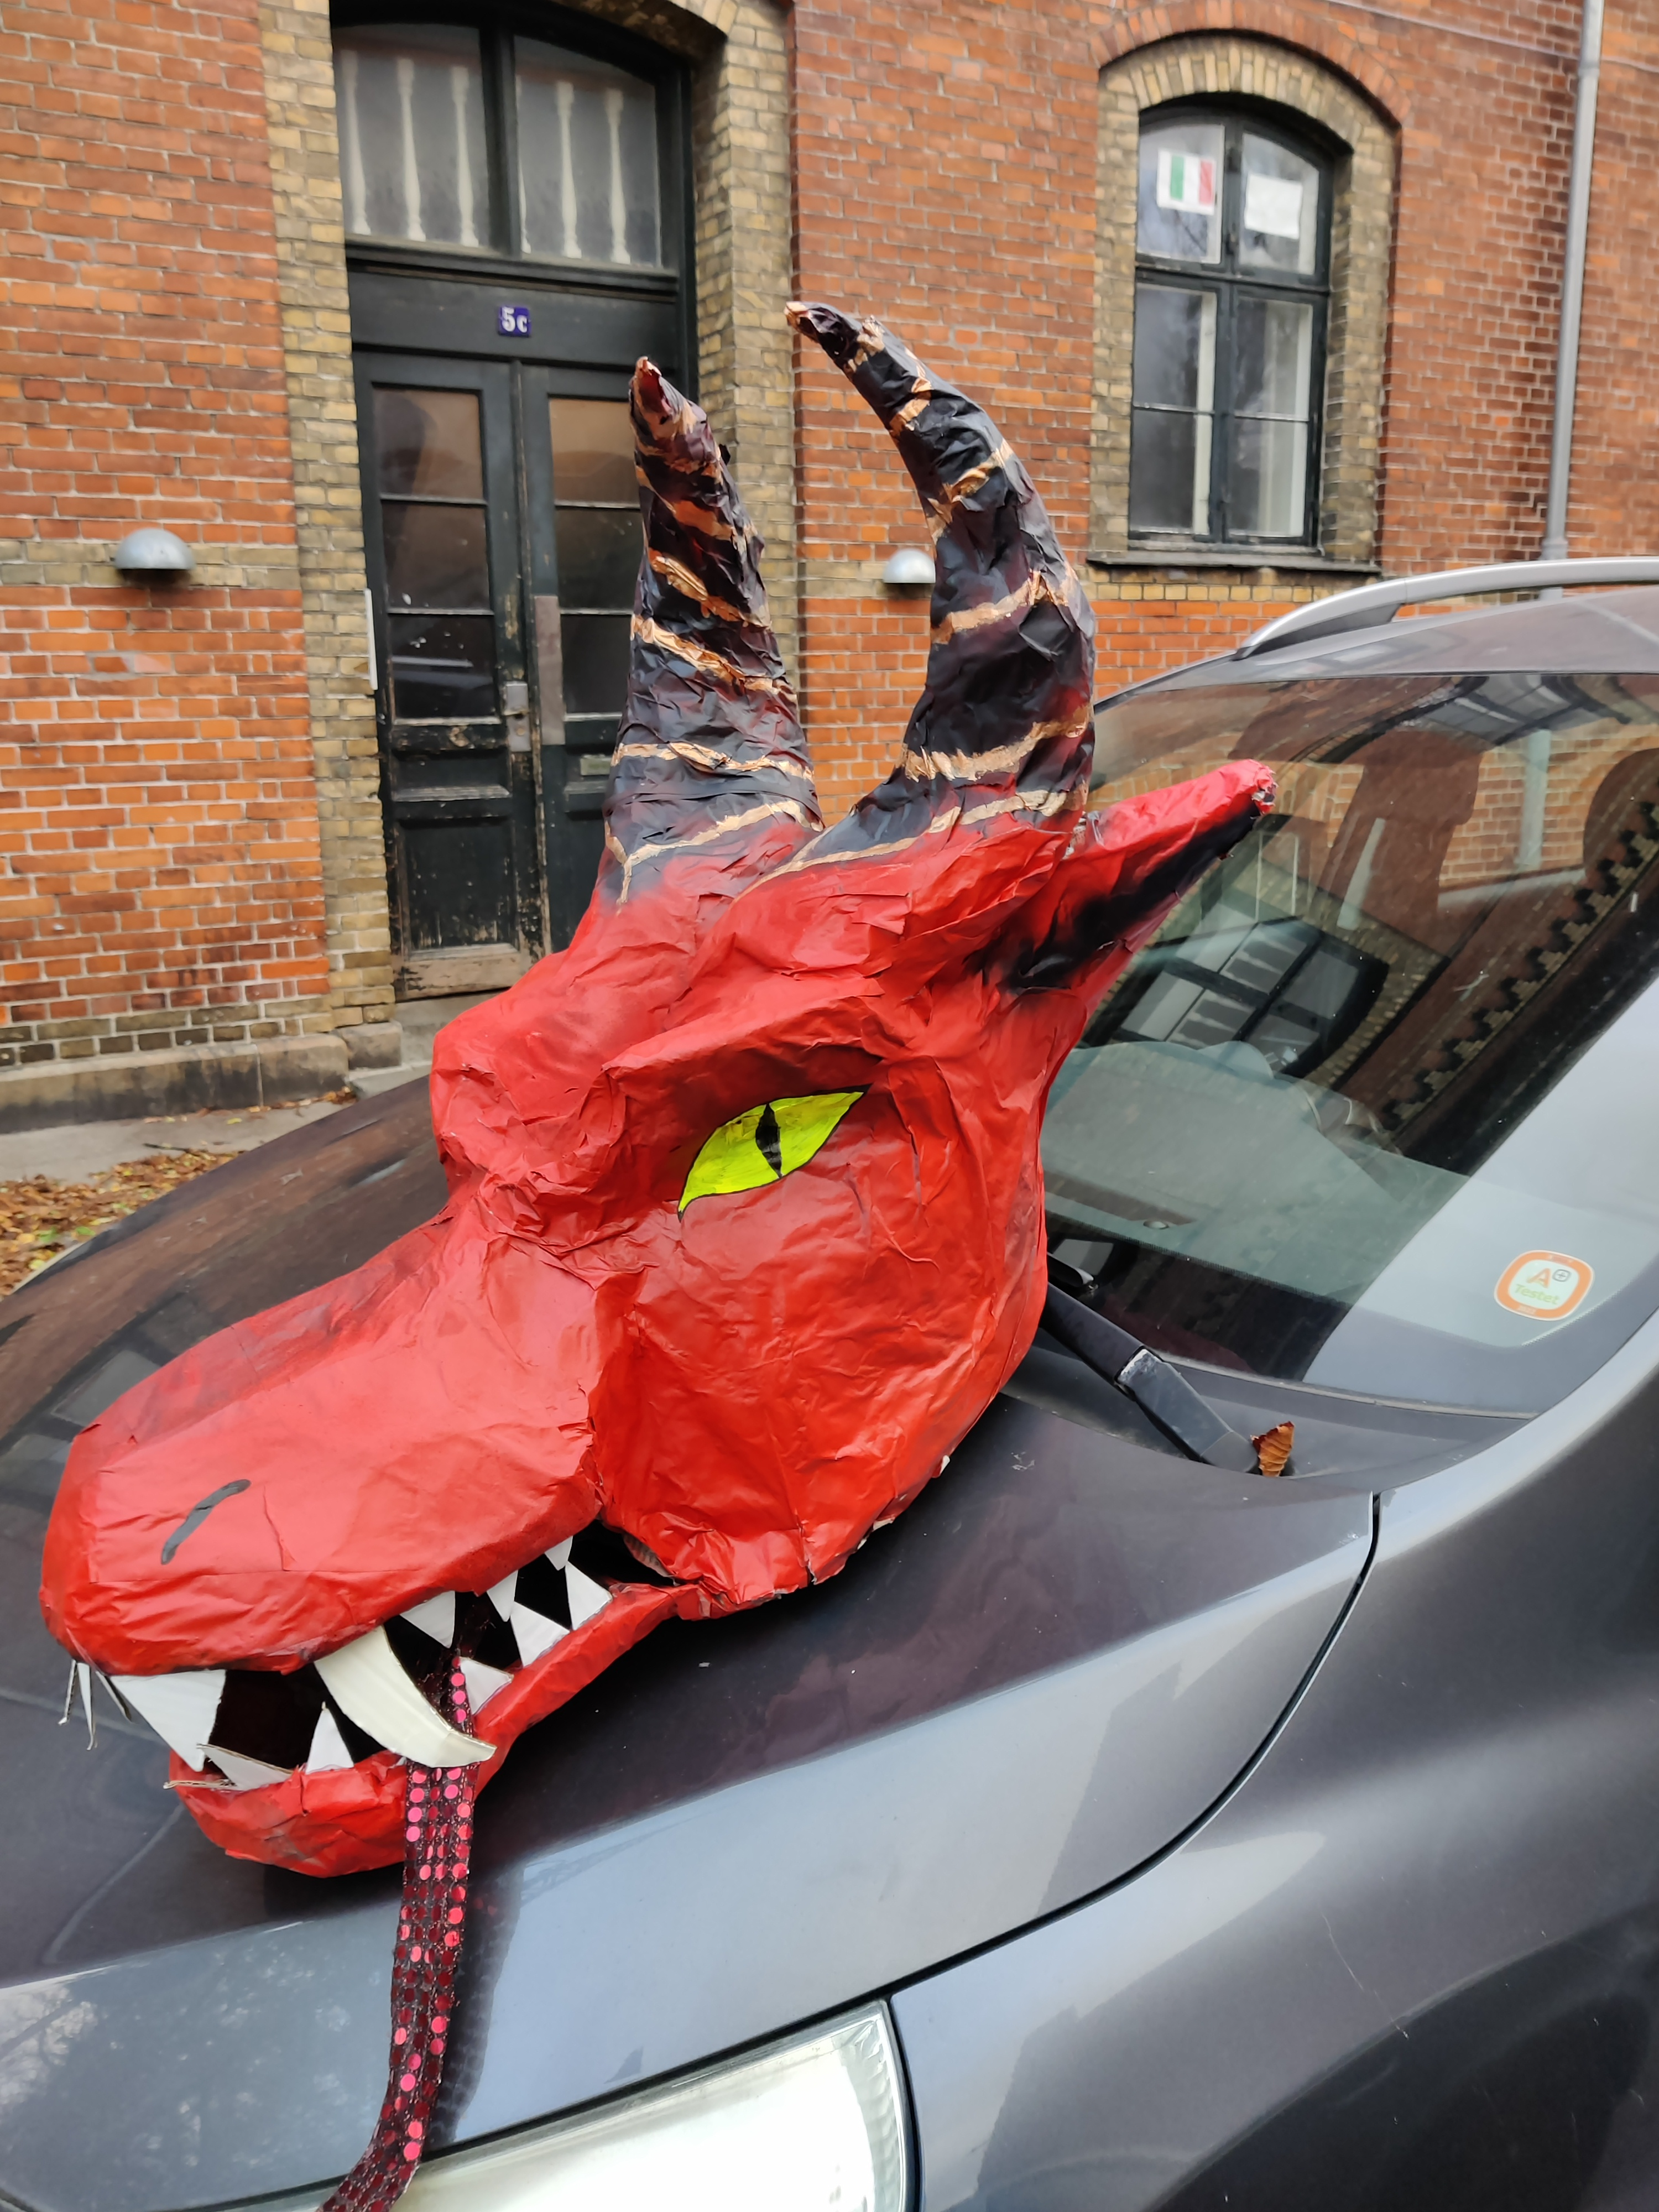
\includegraphics[width=0.5\linewidth]{Helmut.jpg}
    \caption{Dragen Helmut}
  
\end{figure}
\newpage \section{Græsk Yoghurt Dressing}
\begin{minipage}[t]{0.5\textwidth}
\textbf{Ingredienser:}
 \begin{itemize}
        \item 200g græsk yoghurt 10\%
        \item 2 tsk stødt spidskommen
        \item 1 tsk stødt koriander
        \item Salt og peber
    \end{itemize}
\end{minipage}
\begin{minipage}[t]{0.5\textwidth}
\textbf{Fremgangsmåde:}
\begin{enumerate}
    \item Miks alle ingredienser til krydderierne er ligelig fordelt.
\end{enumerate}
\end{minipage}
Til trods for at den her opskrift er super simpel, giver det en super dressing. Har ikke eksperimenteret specielt meget med den, men tænker chiliflager kunne være lækkert.
\newpage 
\begin{tikzpicture}[remember picture,overlay,inner sep=0pt,outer sep=0pt]
    \node[anchor=south east] at (current page.south east) {
        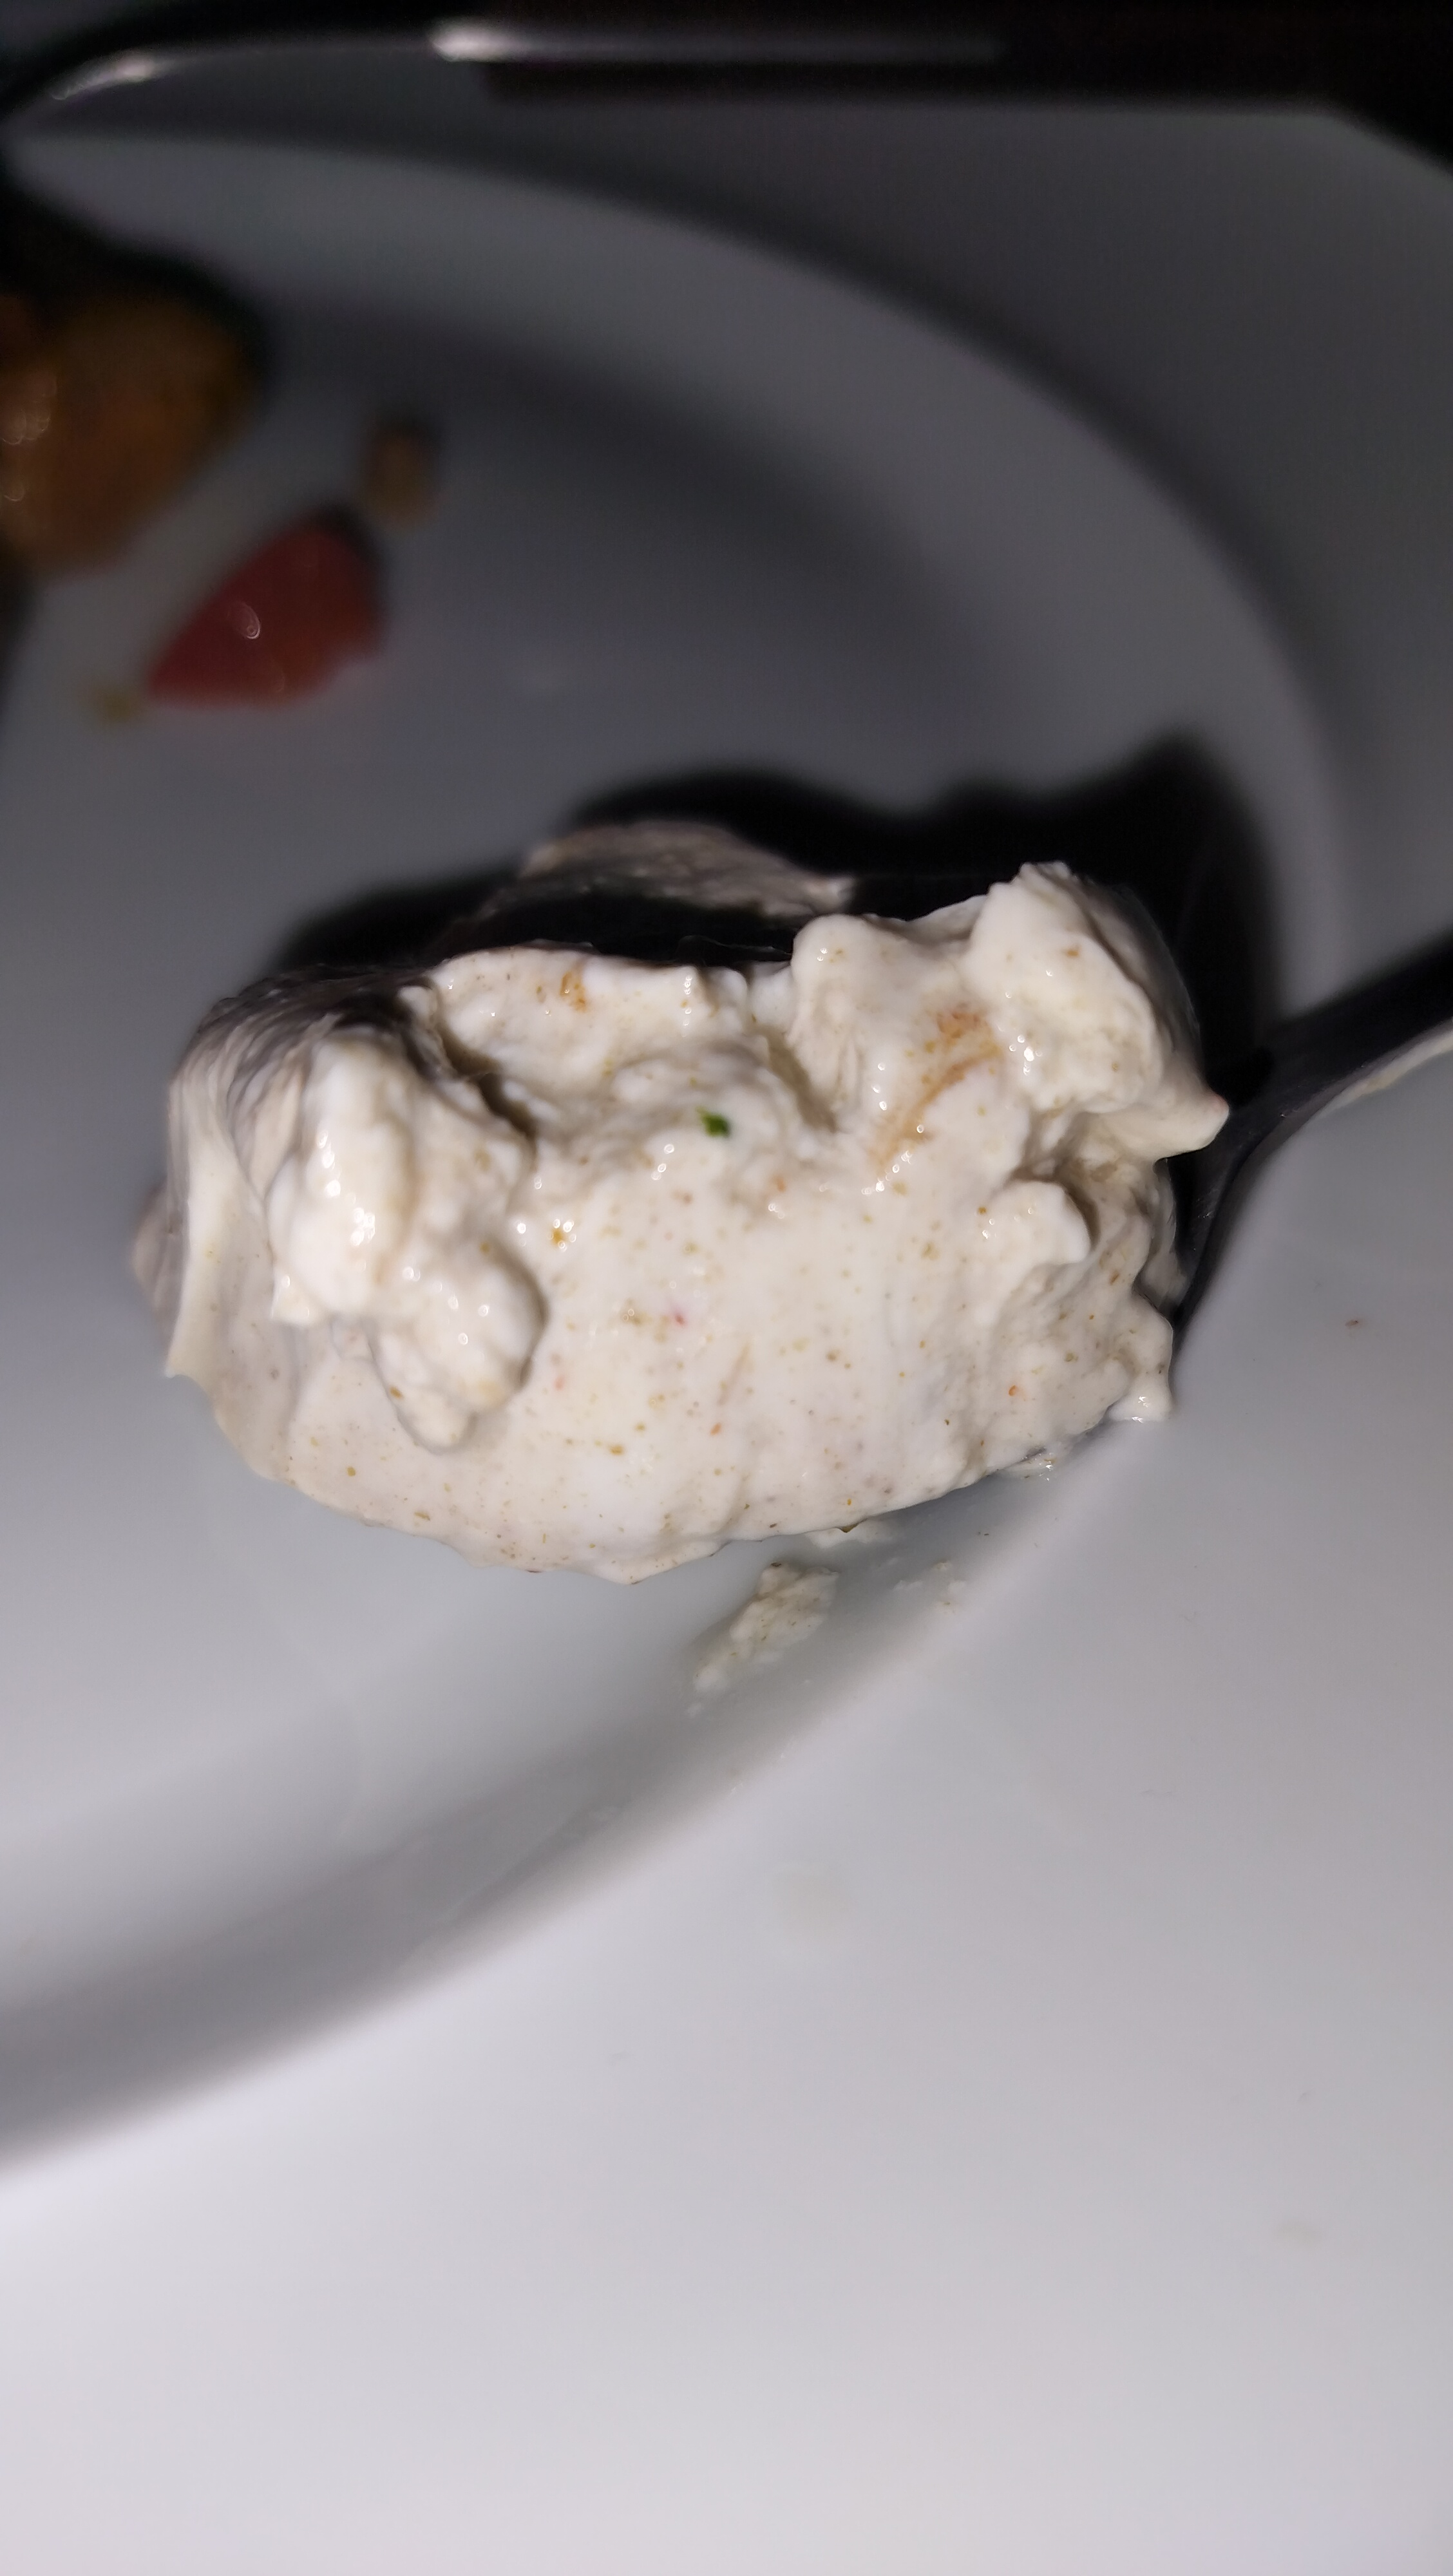
\includegraphics[width=\paperwidth,height=\paperheight]{Billeder/Tilbehør/Græsk_Yoghurt_Dressing.jpg}
    };
\end{tikzpicture}
\newpage \section{Hummus}
\begin{minipage}[t]{0.5\textwidth}
\textbf{Ingredienser:}
\begin{itemize}
    \item 1 dåse kikærter
    \item 1 spsk tahin eller smooth peanutbutter
    \item Citronsaft efter ønske
    \item Mindst 2 fed hvidløg
    \item 1 tsk stødt spidskommen
    \item En smule cayennepeber
    \item 0.5 dL koldt vand (alt efter konsistens)
    \item 3 spsk olivenolie
    \item En smule salt (tahin er meget saltet i sig selv)
    \item Peber
    \item Smag varians
    \begin{itemize}
        \item evt. soltørrede tomater
        \item evt. oliven og kapers
        \item evt. rødbeder
        \item evt. avocado
    \end{itemize}
\end{itemize}
\end{minipage}
\begin{minipage}[t]{0.5\textwidth}
\textbf{Fremgangsmåde:}
\begin{enumerate}
    \item Bland alt sammen minus vand og blend i foodprocessor, tilsæt til sidst vand alt efter konsitens.
    \item Hummus kan med fordel laves med forskellige smage ved at dele hummus portionen i flere portioner og blend de ønskede smage sammen med hummussen.  
\end{enumerate}
\end{minipage}
Som udgangspunkt er Peanut butter en 1:1 erstatning af tahinn, dog er det ikke helt lige så saltet, og giver en svag jordnød smag, dette synes jeg dog let overdøves af de soltørret tomater eller en af de andre smags varianter. Smagsvarianterne skal ses som enten den ene eller den anden, mit forsøg på at lave en oliven og soltørret tomat humus, gav hvert fald bare rød oliven hummus.
\newpage
%\begin{tikzpicture}[remember picture,overlay,inner sep=0pt,outer sep=0pt]
%    \node[anchor=south east] at (current page.south east) {
%        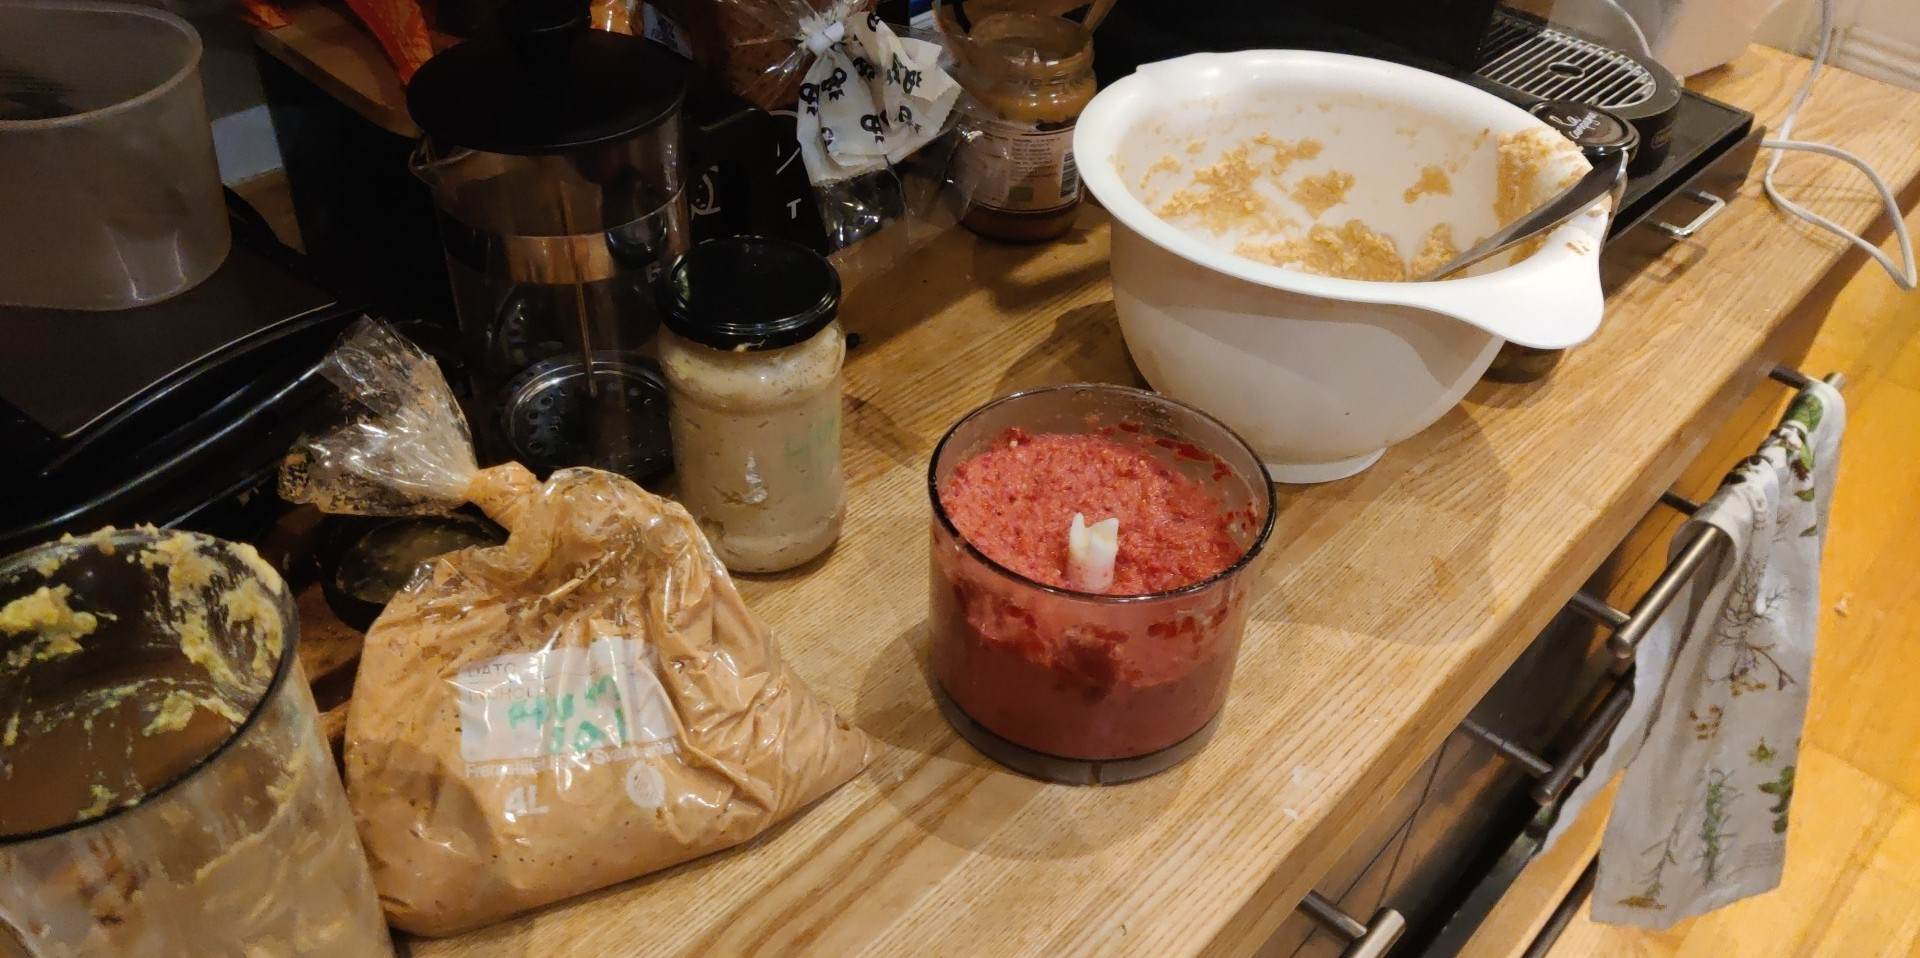
\includegraphics[width=\paperwidth,height=\paperheight]{Billeder/Tilbehør/Hummus.jpeg}
%    };
%\end{tikzpicture}
Billedet af hummus er desværre ikke i den ønskede opløsning, så derfor er layout af dette en smule anderledes end hvad jeg ellers ønsker.
\begin{figure}[h]
    \centering
    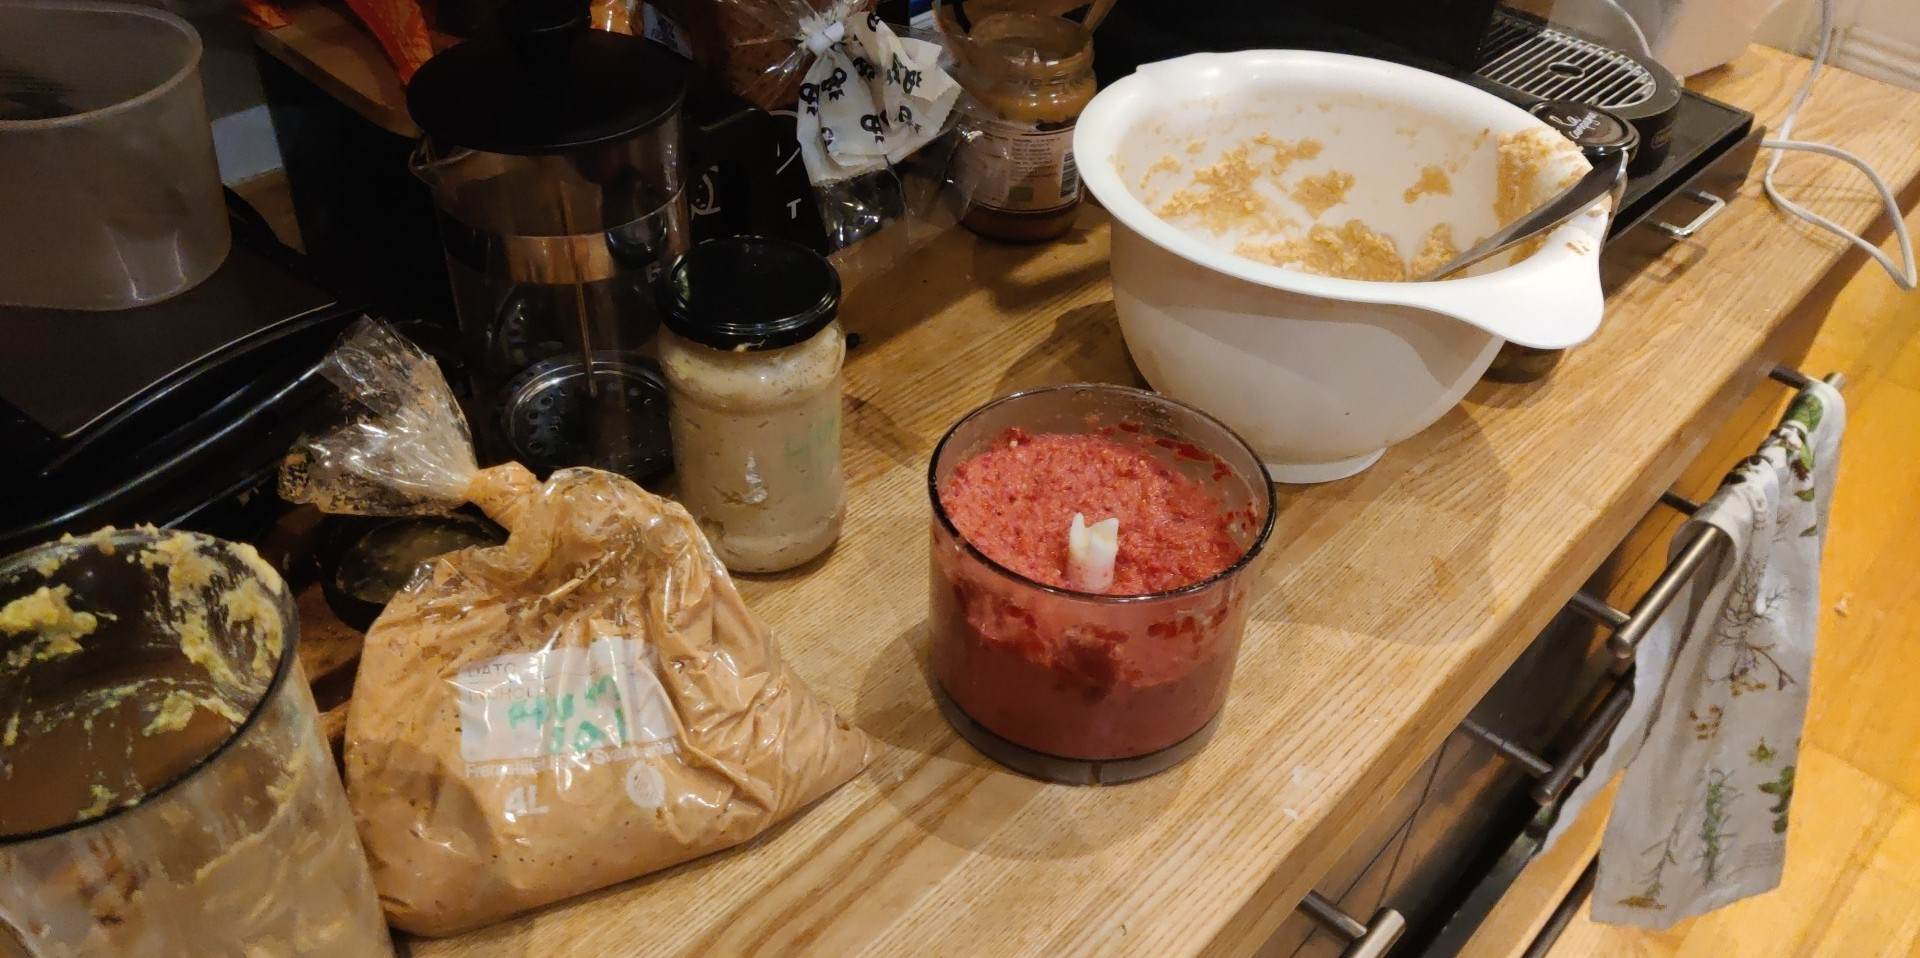
\includegraphics[width=0.75\linewidth]{Billeder/Tilbehør/Hummus.jpeg}
    \caption{4 forskellige salgs hummus}
    \label{fig:enter-label}
\end{figure}
\newpage \section{Hvidløgssmør}
\begin{minipage}[t]{0.5\textwidth}
\textbf{Ingredienser:}
\begin{itemize}
    \item 200 gram smør
    \item 4-5 fed hvidløg, hakket eller presset
\end{itemize}
\end{minipage}
\begin{minipage}[t]{0.5\textwidth}
\textbf{Fremgangsmåde:}
\begin{enumerate}
    \item Blød smørret til den kan æltes
    \item Pres eller hak hvidløgene, og fordel så jævnt som muligt.
    \item Stil på køl til det skal bruges.
\end{enumerate}
\end{minipage}
\textcolor{white}{white} \\
Denne opskrift er relativ simpel, men der er et par ting man skal være opmærksom på. Smørret skal helst være blødt, man kan, som udgangspunkt, godt smelte smørret og tilføje hvidløget, men dette giver en lidt underlig konsistens til hvidløgssmøret, vil dermed anbefale at man lader det stå ude i 20-30 minutter, og så mikser det enten med hænderne eller spisepinde. 
\newpage \begin{tikzpicture}[remember picture,overlay,inner sep=0pt,outer sep=0pt]
    \node[anchor=south east] at (current page.south east) {
        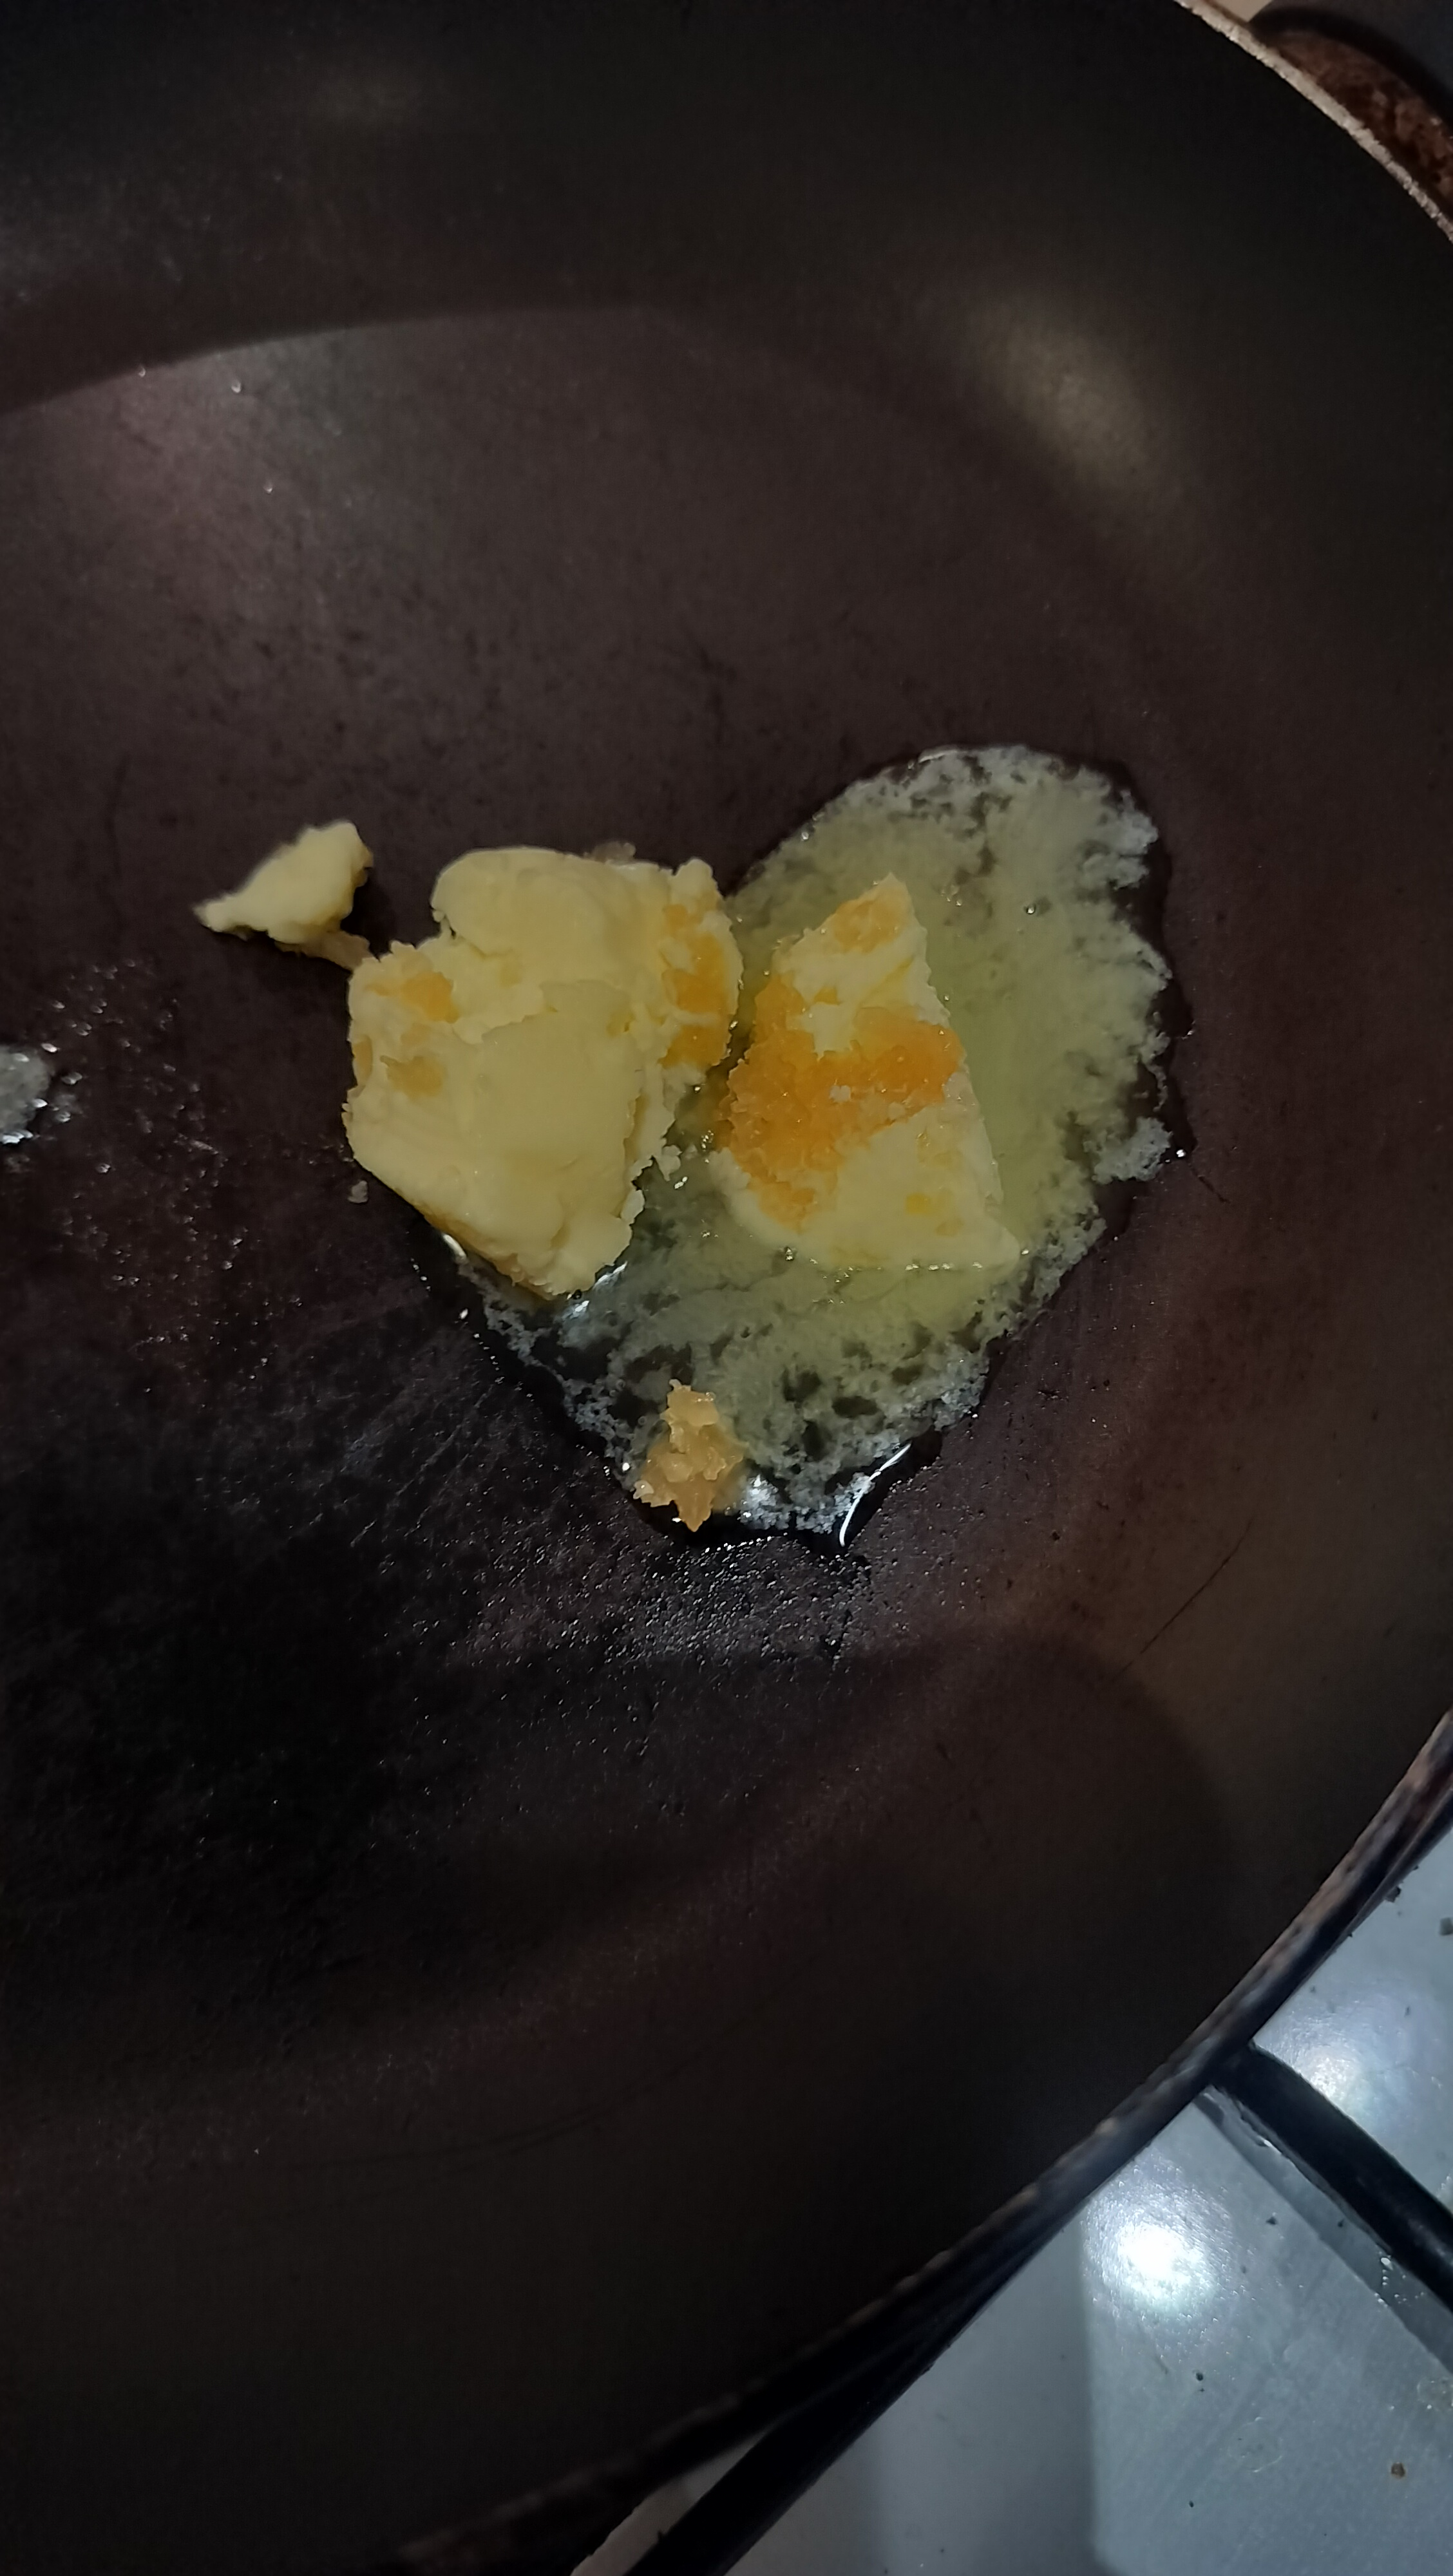
\includegraphics[width=\paperwidth,height=\paperheight]{Billeder/Tilbehør/Hvidløgssmør.jpg}
    };
\end{tikzpicture}
\newpage \section{Oliventapenade}
\begin{minipage}[t]{0.5\textwidth}
\textbf{Ingredienser:}
\begin{itemize}
    \item 200g sorte oliven
    \item 2 spsk olivenolie
    \item kapers
    \item 3 fed hvidløg
\end{itemize}
\end{minipage}
\begin{minipage}[t]{0.5\textwidth}
\begin{enumerate}
    \item Tilsæt alle ingredienserne og blend i foodprocessor til ønskede konsistens
\end{enumerate}
\end{minipage}
Jeg synes personligt at det er lækkert når olivener er i små stykker, men stadig mere individuelt.
\newpage Her skulle der så også være et billede, så vi tager en (potentielt) anden måge i Oslo
\begin{figure}
    \centering
    \rotatebox{270}{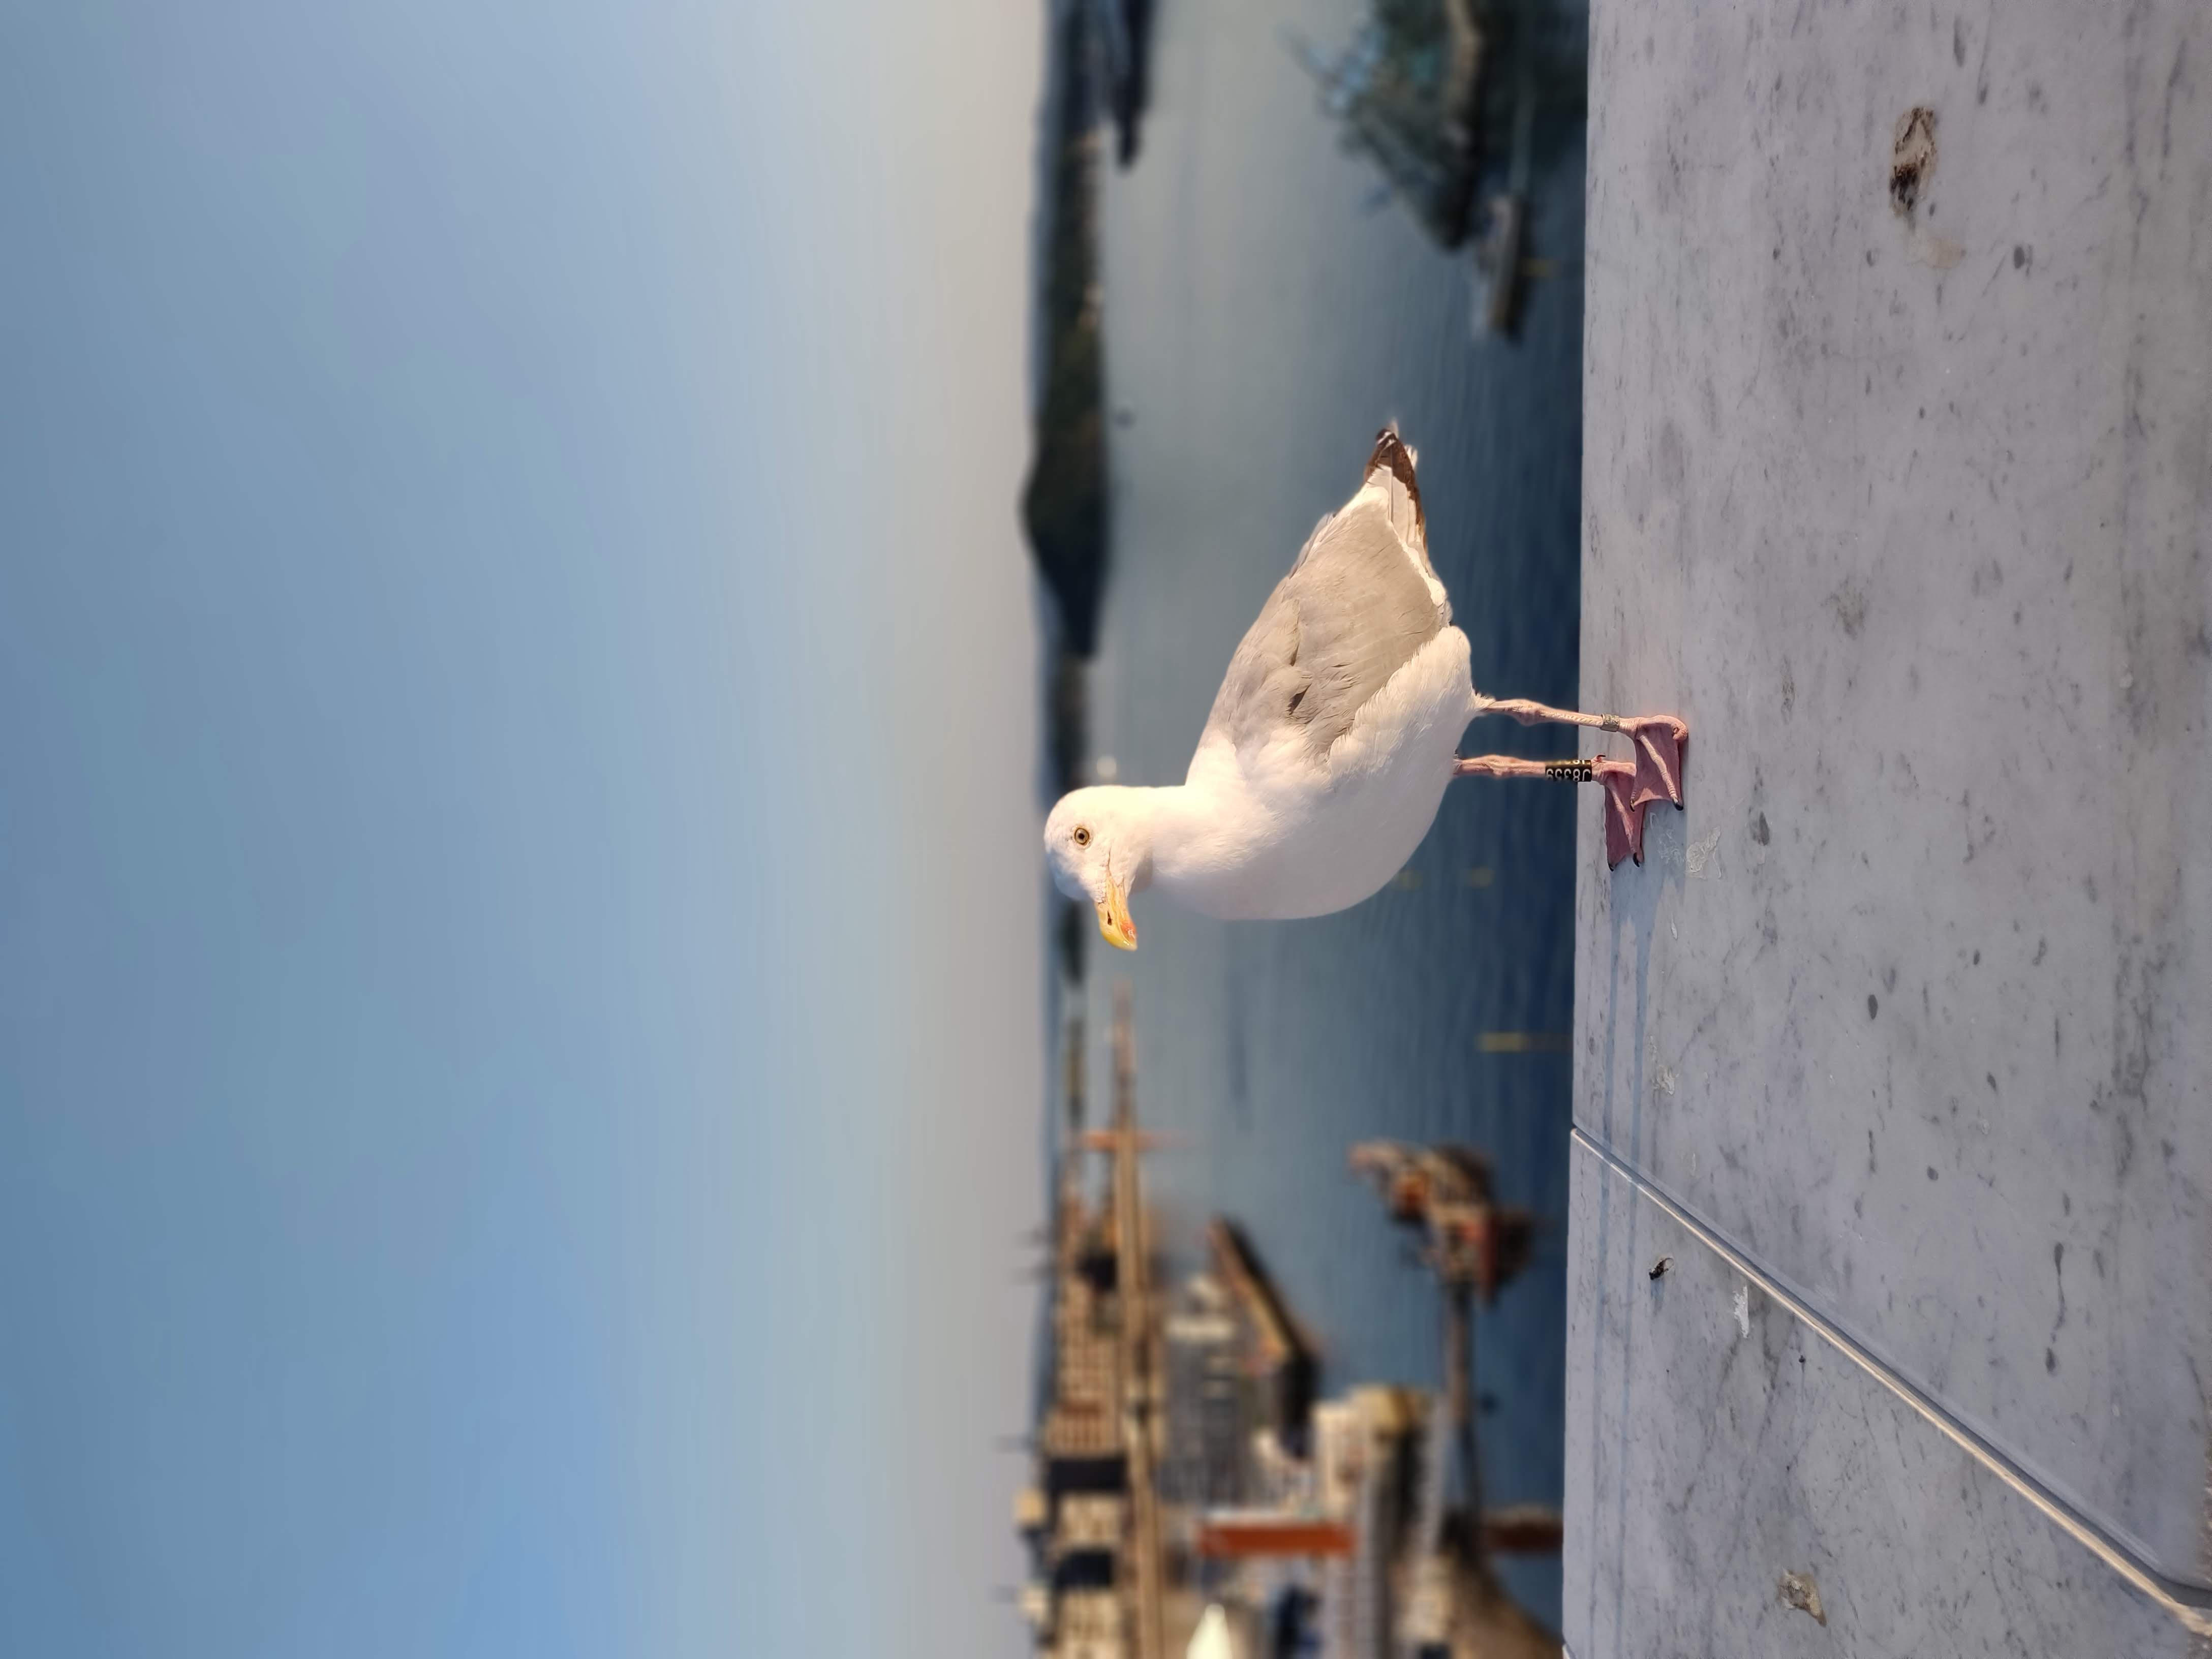
\includegraphics[width=0.5\linewidth]{Måge2.jpg}}
    \caption{Måge nr 2}
\end{figure}
\newpage \section{Pico de Gallo}
\begin{minipage}[t]{0.5\textwidth}
\textbf{Ingredienser:}
\begin{itemize}
    \item 3-4 tomater, skåret i tern
    \item 1-2 rødløg, skåret i tern
    \item 0.5 håndfuld friske koriander
    \item 1 fed hvidløg, presset
    \item Citron- eller limesaft
    \item Salt og pbber
\end{itemize}
\end{minipage}
\begin{minipage}[t]{0.5\textwidth}
\begin{enumerate}
    \item Dræn tomaterne for noget af væden.
    \item Miks alle ingredienserne i en skål.
    \item Lad stå på køl i helst en time, gerne længere
\end{enumerate}
\end{minipage}
\newpage 
\begin{tikzpicture}[remember picture,overlay,inner sep=0pt,outer sep=0pt]
    \node[anchor=south east] at (current page.south east) {
        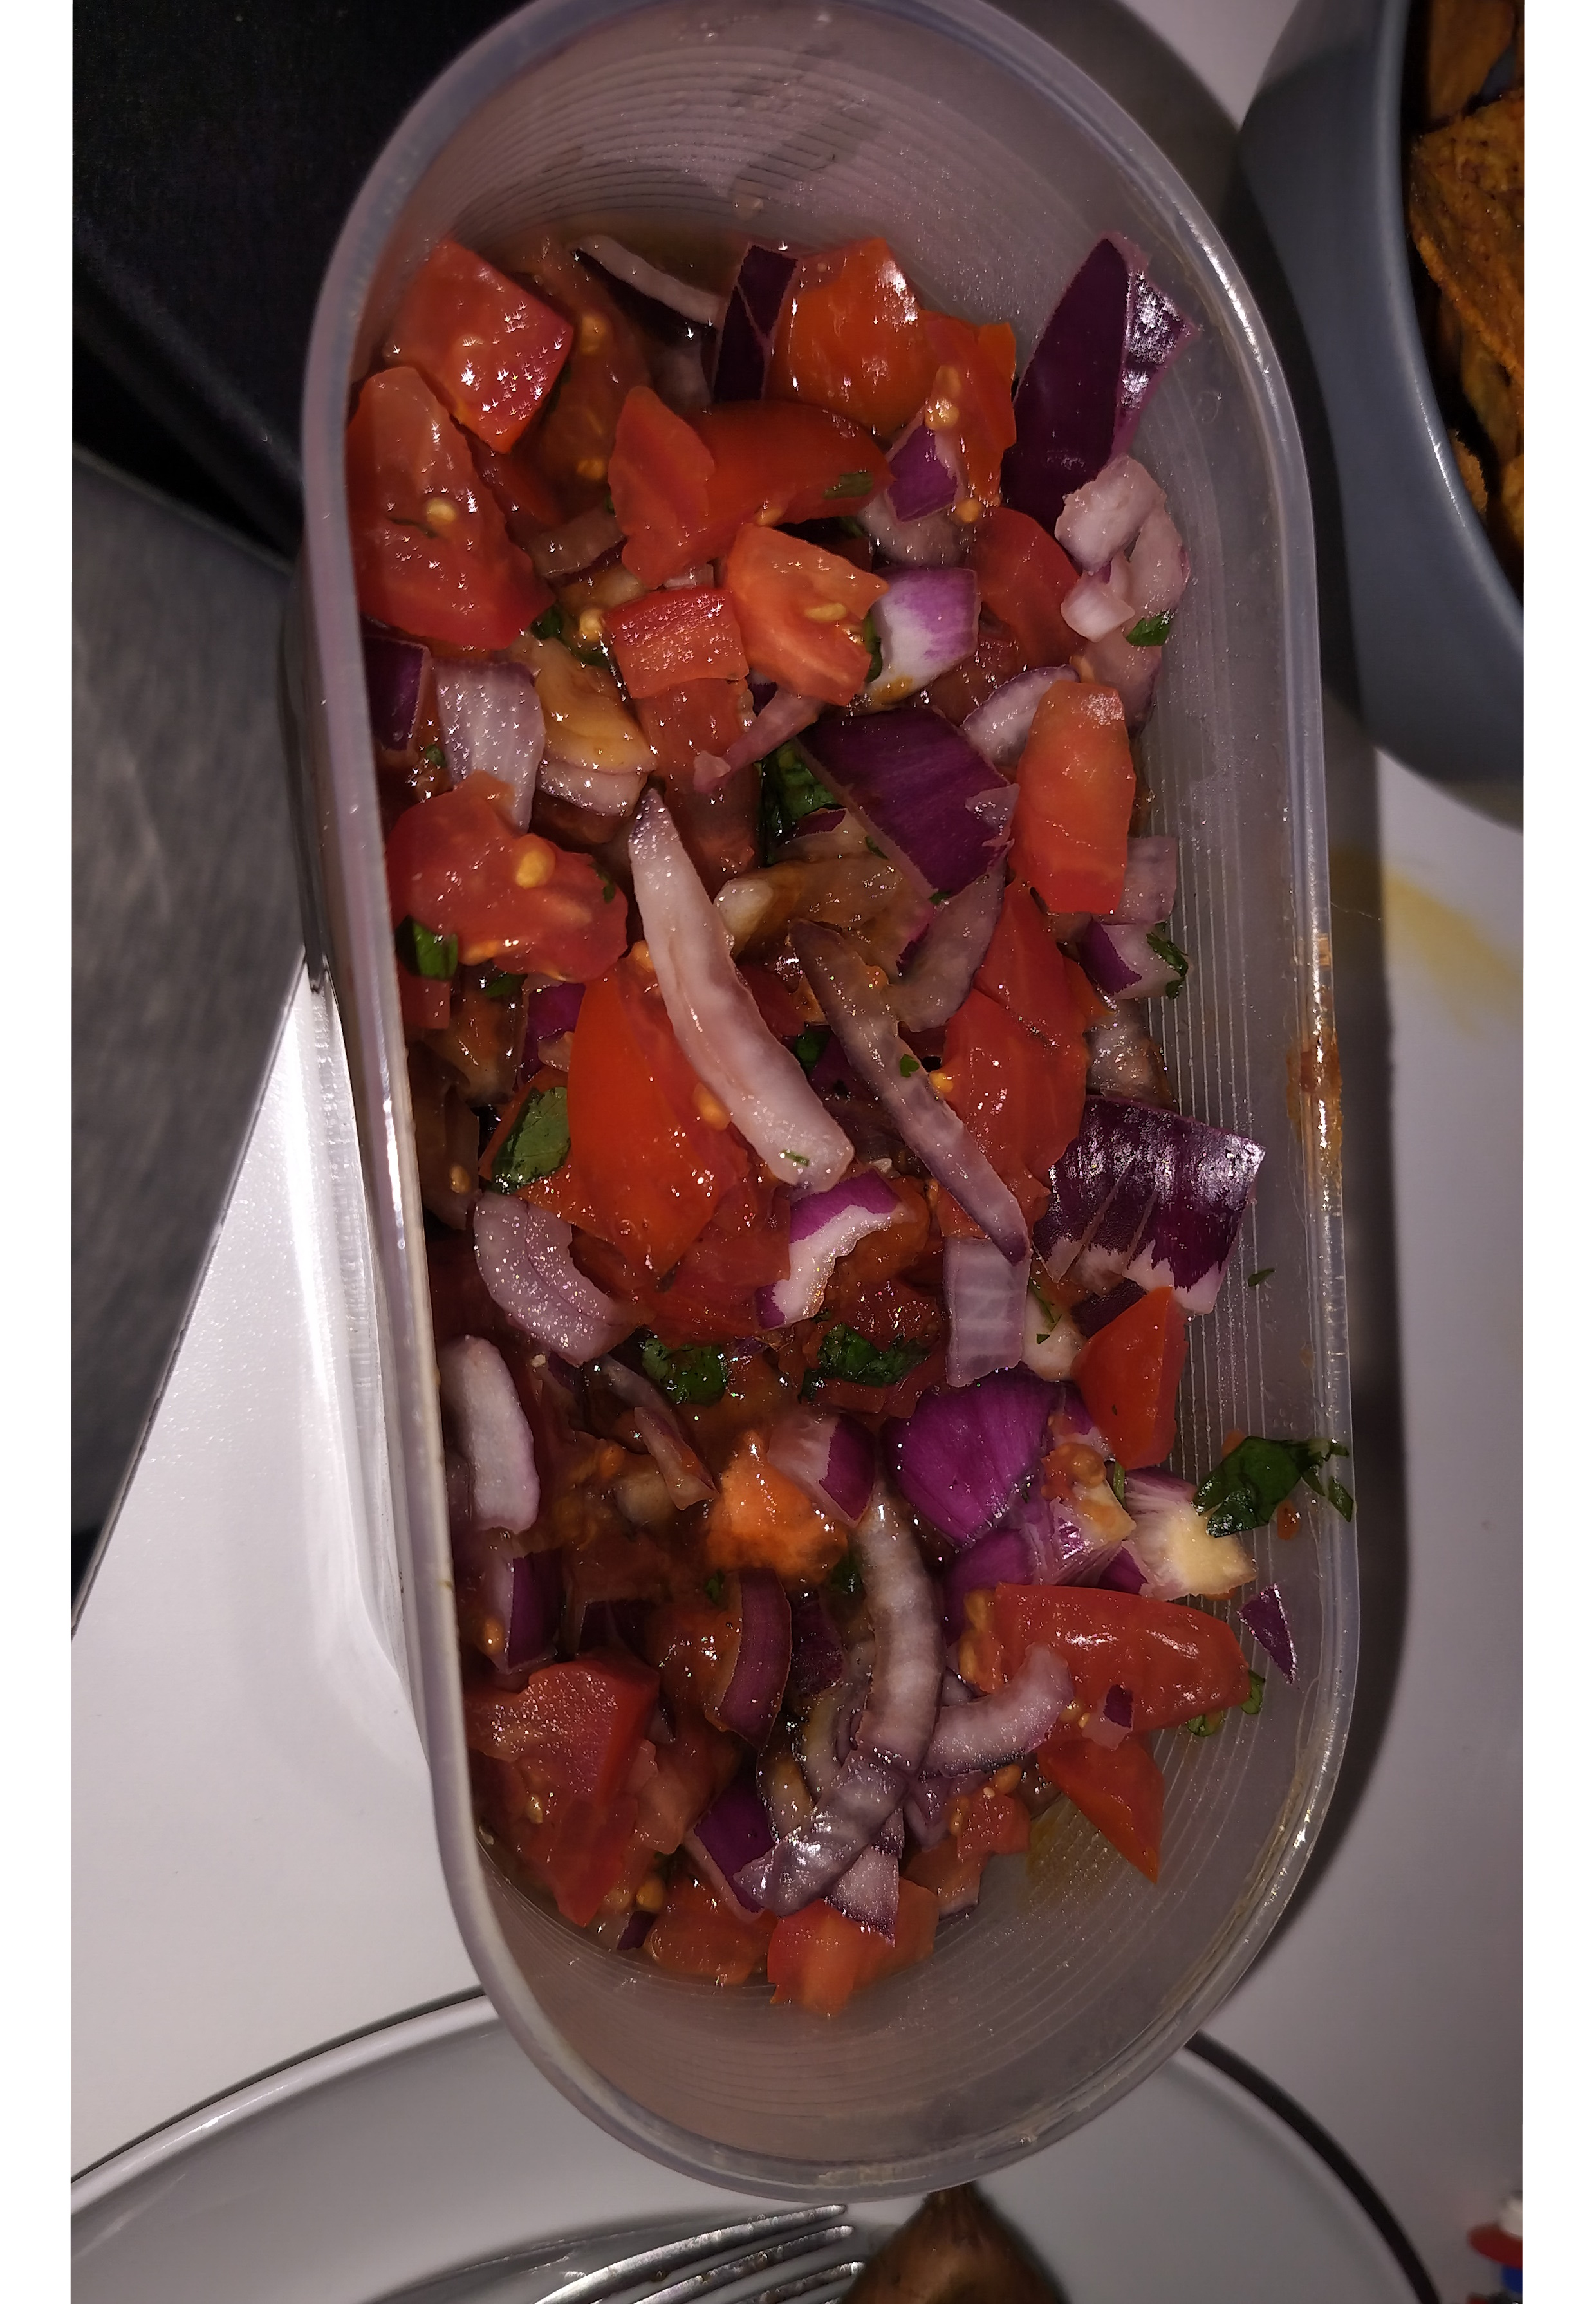
\includegraphics[width=\paperwidth,height=\paperheight]{Billeder/Tilbehør/Pico2.jpg}
    };
\end{tikzpicture}
\newpage\section{Portobello Svampe med Ost}
\begin{minipage}[t]{0.5\textwidth}
\textbf{Ingredienser:}
\begin{itemize}
    \item Portobello Svamp (helst relativ store)
    \item En eller flere af de følgende ost
    \begin{enumerate}
        \item Gedeost
        \item Mozzarella kugle
        \item Blå ost
    \end{enumerate}
\end{itemize}
\end{minipage}
\begin{minipage}[t]{0.5\textwidth}
\begin{enumerate}
    \item Vask portobello svampene, fjern stilken og eventuel lamellerne
    \item Den fjernet stilk og de eventuelle lameller kan skæres i stykker og blandes sammen med den ønskede ost
    \item Steg i ovnen eller på grillen til osten er smeltet (\~15 minutter ved 200 \degree C varmluft)
\end{enumerate}
\end{minipage}
Til denne opskrift er der ikke det store af mål, da det kommer an på hvor ostet man vil have det. Med mozzarella kan en kugle med fordel bruges til 2-3 portobello svampe.
\newpage Her er der et billede af Andrey, i stedet for et billede af portobello svampe med ost.
\begin{figure}
    \centering
    
\includegraphics[width=0.5\linewidth]{Andrey.jpg}
    \caption{Andrey til pride}
\end{figure}
\newpage \section{Svampe Sauce}

\begin{minipage}[t]{0.5\textwidth}
\textbf{Ingredienser:}
\begin{itemize}
    \item 2 spsk smør
    \item 1/2 spsk olivenolie
    \item 300 g champignoner hakket 
    \item 2-3 fed hvidløg, presset
    \item Et skvat hvidvin
    \item 125 mL grøntsagsbouillon
    \item 50 g parmassen
    \item timian
    \item salt og peber
\end{itemize}
\end{minipage}
\begin{minipage}[t]{0.5\textwidth}
\textbf{Fremgangsmåde:}
\begin{enumerate}
    \item Smelt smørret og varm olien i en gryde sammen med svampene ved høj varme.
    \item Når de er blødt tilsæt hvidløget.
    \item Hæl vinen i under omrøring.
    \item Tilsæt grøntsagsbouillonen, fløden og parmesanen, og skru ned for varmen.
    \item Rør i 2-3 minutter, og smag til med timian, salt og peber.
\end{enumerate}
\end{minipage}
\newpage \begin{tikzpicture}[remember picture,overlay,inner sep=0pt,outer sep=0pt]
    \node[anchor=south east] at (current page.south east) {
        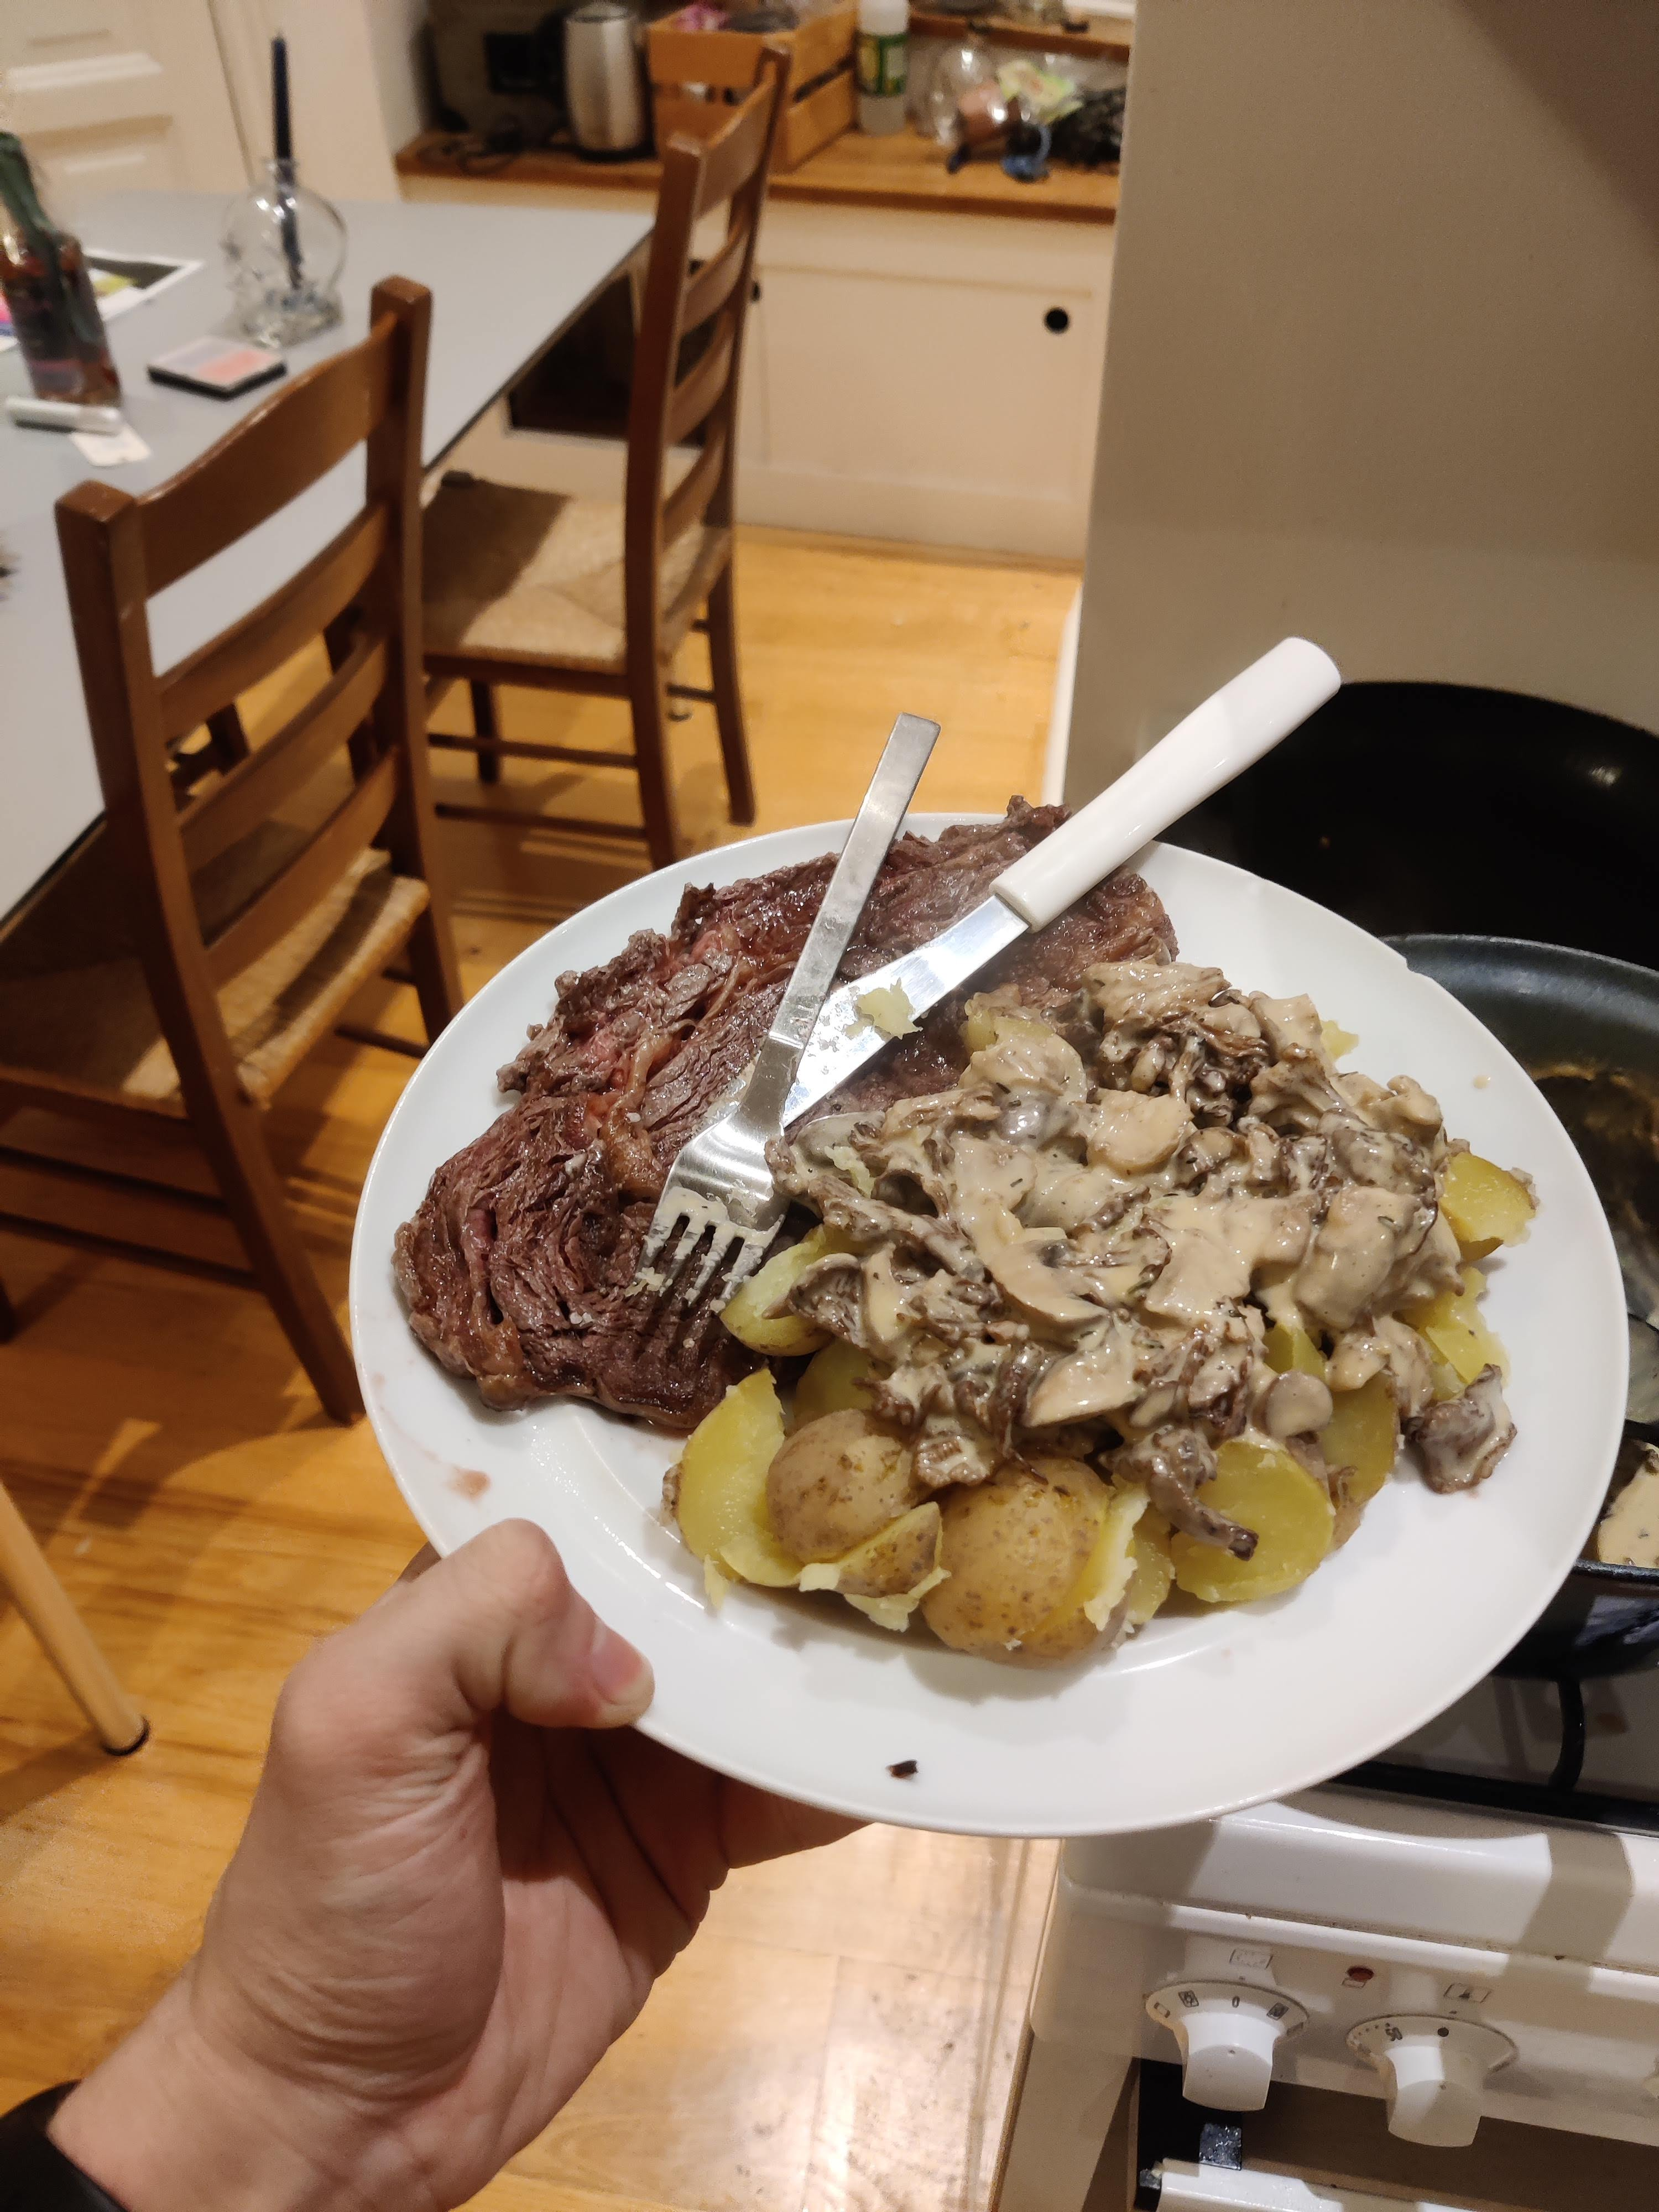
\includegraphics[width=\paperwidth,height=\paperheight]{Billeder/Tilbehør/Svampesauce.jpg}
    };
\end{tikzpicture}
\newpage \section{Tzaziki/Raita}
\begin{minipage}[t]{0.5\textwidth}
\textbf{Ingredienser:}
\begin{itemize}
    \item 1/2 agurk
    \item 1 håndfuld frisk mynte
    \item 2 fed hvidløg
    \item 200 mL græsk yoghurt 10 \% (teknisk set yoghurt naturel til raita)
    \item salt og peber
    \item Eventuelt en smule citronsaft
\end{itemize}
\end{minipage}
\begin{minipage}[t]{0.5\textwidth}
\textbf{Fremgangsmåde:}
\begin{enumerate}
    \item Riv agurken på et mandolin jern til tynde skiver.
    \item Mas så meget af væsken som muligt ud af agurkeskiverne.
    \item Bland dernæst alle ingredienserne, og server køligt.
\end{enumerate}
\end{minipage}
\newpage 
Igen mangler desværre et billede 
\begin{figure}
    \centering
    \includegraphics[width=0.5\linewidth]{Lego.jpg}
    \caption{Mig der, i et shopping center i Virginia, fandt en LEGO® butik}
    
\end{figure}
\newpage \section{Hvide Asparges i Brunet Smør}
\begin{minipage}[t]{0.5\textwidth}
\begin{itemize}
    \item 200g hvide asparges 
    \item 50g smør
    \item Salt
\end{itemize}
\end{minipage}
\begin{minipage}[t]{0.5\textwidth}
\begin{enumerate}
    \item Smelt smørret i en kasserolle.
    \item Dernæst bag de hvide asparges i ovnen ved 200 \degree C dækkede af det brunede smør
\end{enumerate}
\end{minipage}
\newpage 
Og desværre også her 
\begin{figure}
    \centering
    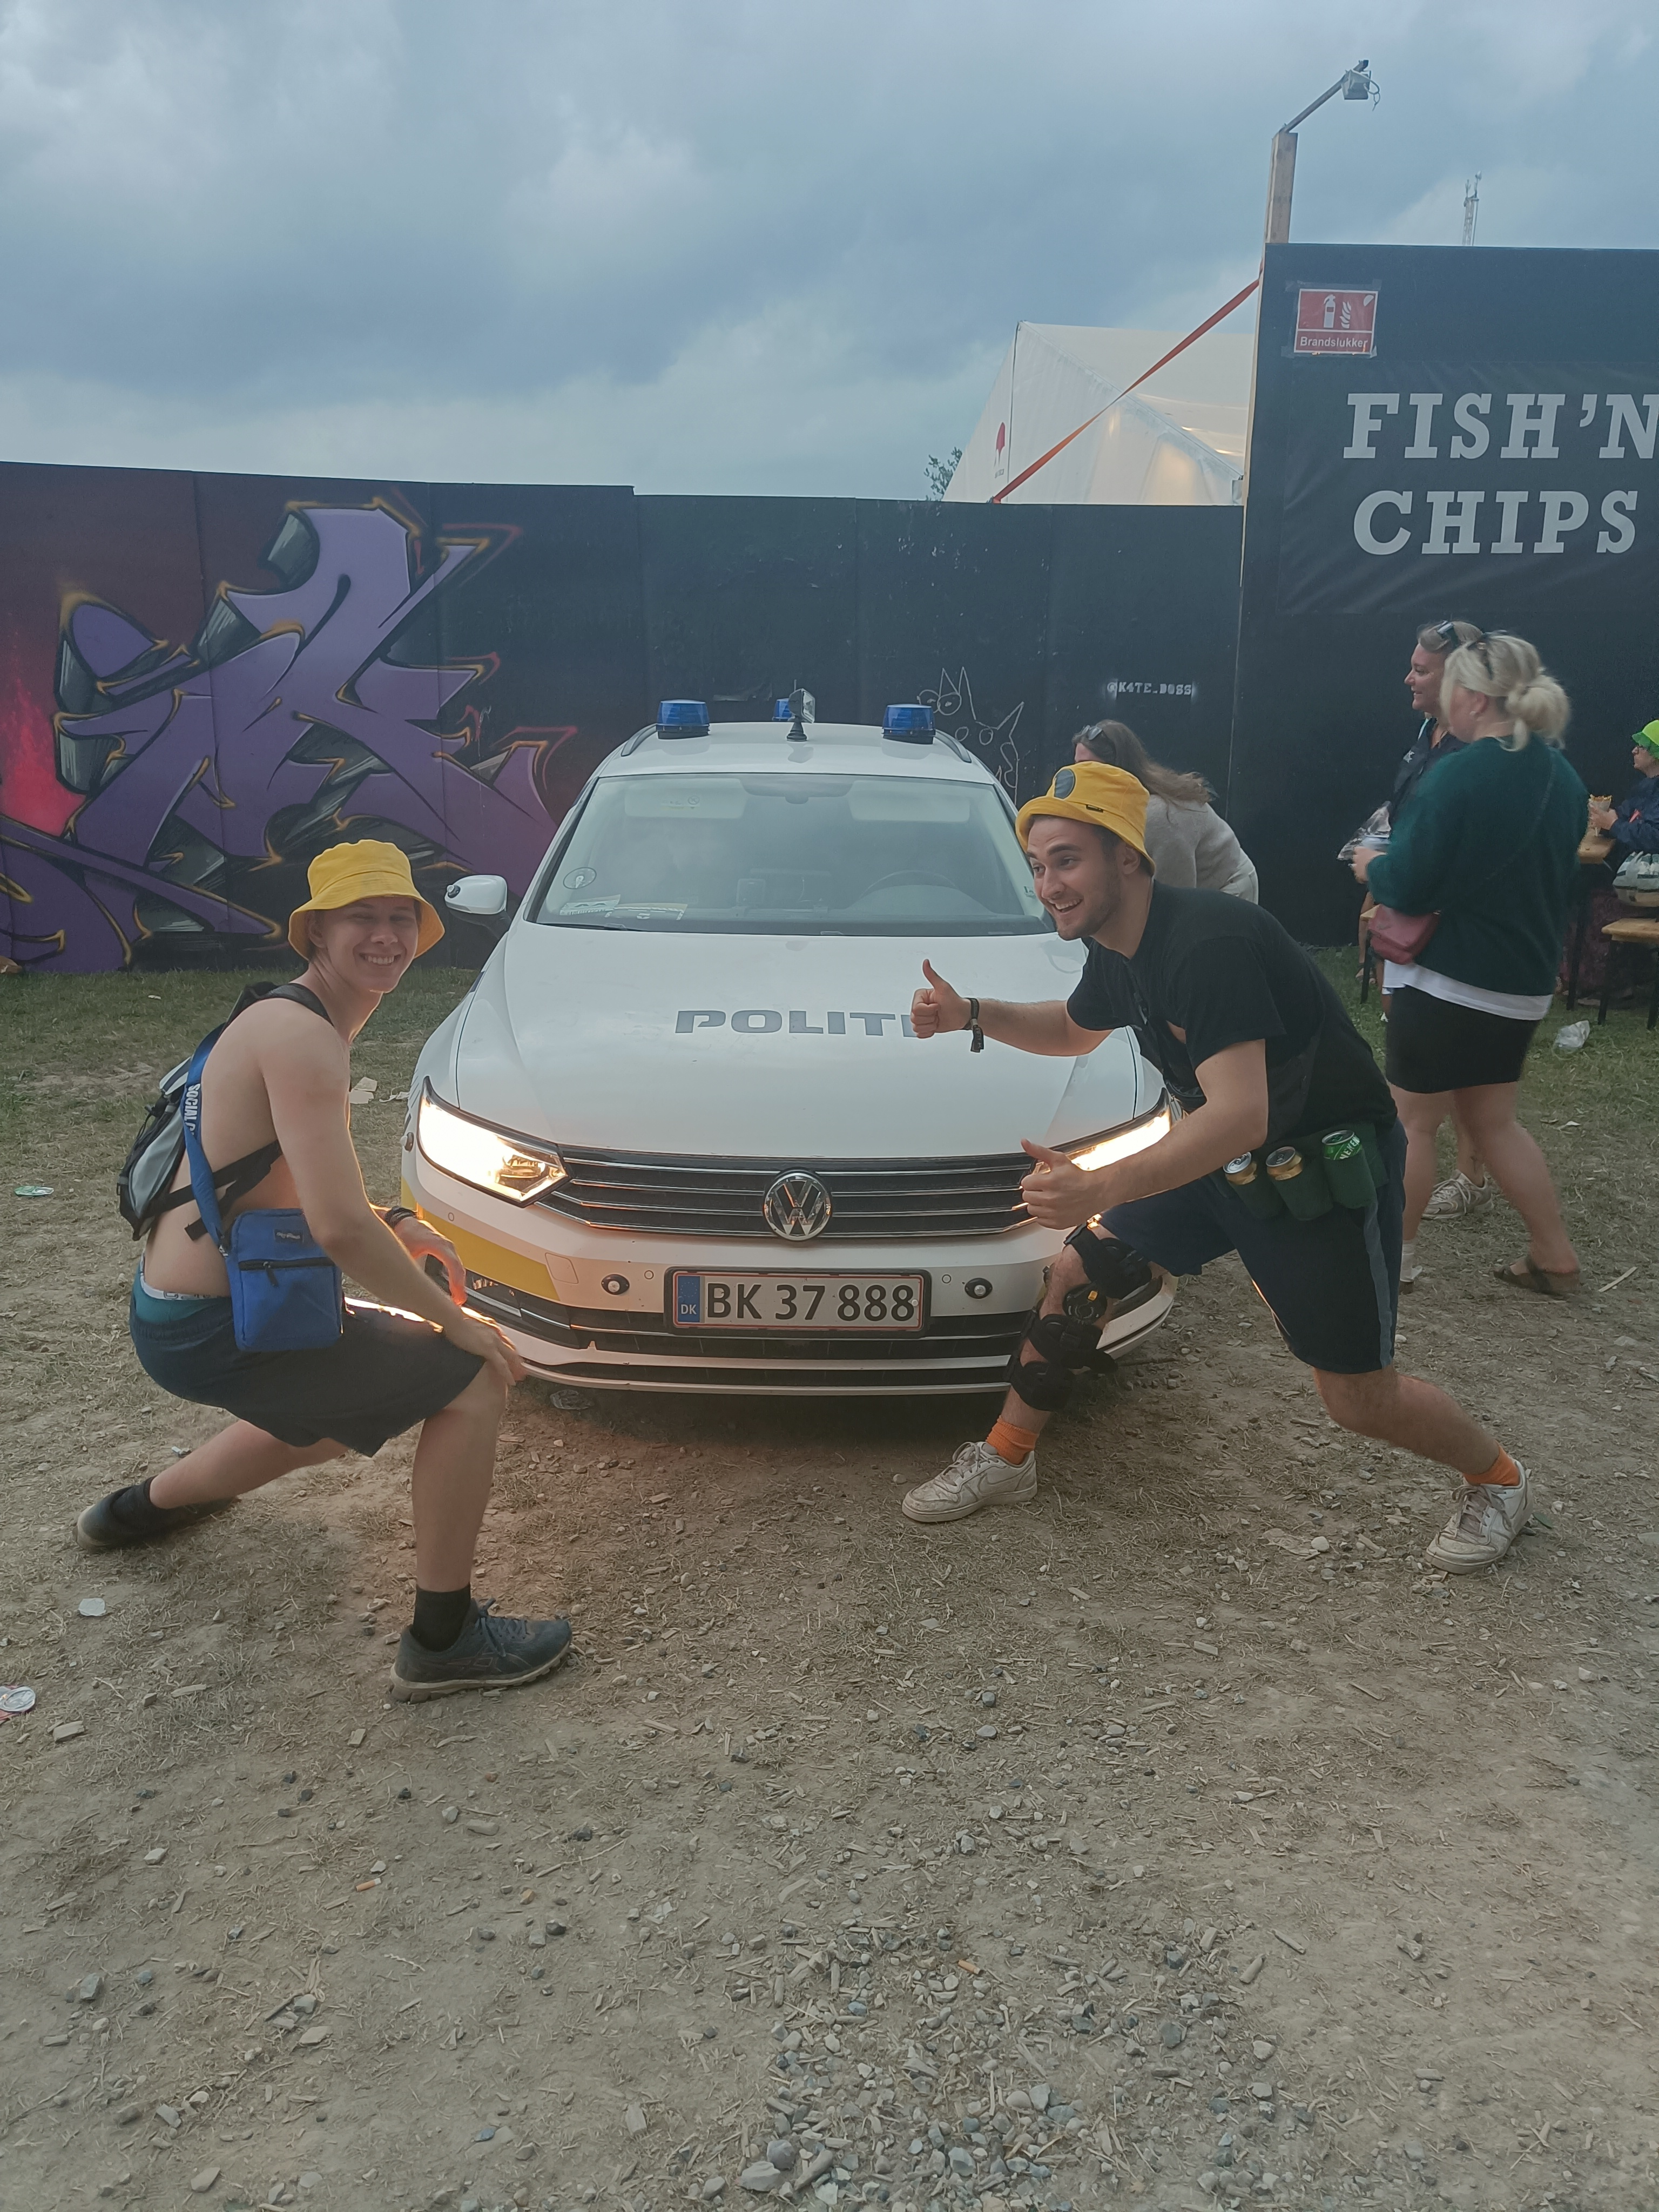
\includegraphics[width=0.5\linewidth]{Roskilde.jpg}
    \caption{Andrey og jeg foran en politi bil på Roskilde}
    
\end{figure}
\chapter{De søde sager}
\minitoc
\newpage\section{Banankage}
\begin{minipage}[t]{0.5\textwidth}
\textbf{Ingredienser:}
\begin{itemize}
  \item 150g smør
  \item 175 g sukker
  \item 1 tsk vaniljesukker
  \item 4 æg
  \item 5 banan, meget modne
  \begin{itemize}
    \item evt. 75g hakket chokolade
    \item evt. 40g val- eller hasselnødder
  \end{itemize}
  \item  175 g hvedemel
   \item1  tsk bagepulver
   \item 1 knivspids salt 
\\ \underline{Topping:}
 \item 100g Smeltet chokolade
\begin{itemize}
    \item evt. 80g hakket hasselnødder
    \item evt. en smule flormelis
\end{itemize} 
\end{itemize}
\end{minipage}
\begin{minipage}[t]{0.5\textwidth}
\textbf{Fremgangsmåde:}
\begin{enumerate}
   \item  Start med at smelte smørret og pisk sammen med sukker og vaniljesukker. 
   \item  Mos bananerne og tilsæt.
   \item  Dernæst tilsæt æggene et ad gangen og chokolade og sukker.
   \item  Rør bagepulver, mel og saltet i.
   \item  Hæld dejen i den ønskede form (f.eks. en springform med smurte sidder, ellers kan en bradepande også gå an), og smid i ovnen på 175 \degree C i 45 minutter
   \item  Hæld den smeltede chokolade på den varme kage og drys de hakkede nødder på 
\end{enumerate}
\end{minipage}
Hvis man ønsker at lave banankage, men ikke har nogle overmodne bananer, kan man få den samme effekt ved at smide dem i fryseren, dette nedbryder cellevæggen.
\newpage
\begin{tikzpicture}[remember picture,overlay,inner sep=0pt,outer sep=0pt]
    \node[anchor=south east] at (current page.south east) { 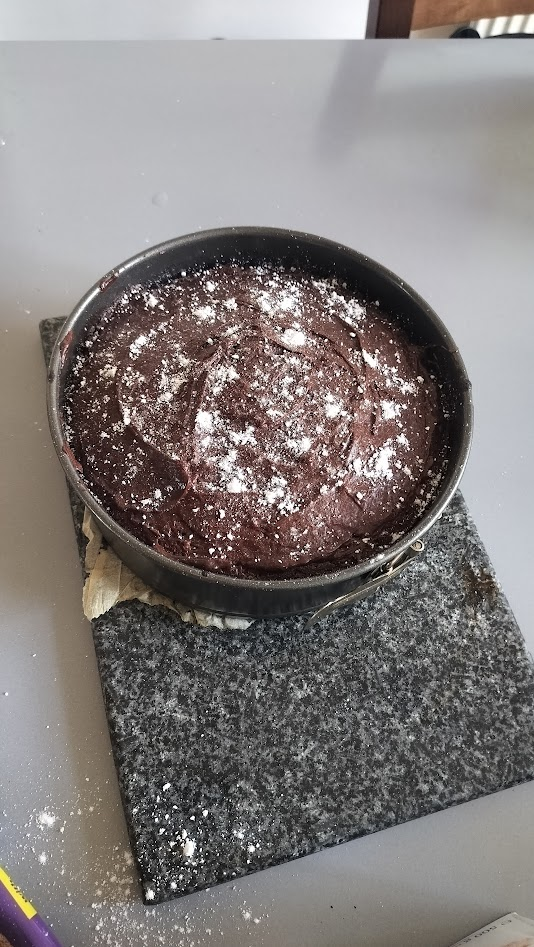
\includegraphics[width=\paperwidth,height=\paperheight]{Billeder/Dessert/banankage2.jpg} };
\end{tikzpicture}

\newpage \section{Brownie}
\begin{minipage}[t]{0.5\textwidth}
\textbf{Ingredienser:}
\begin{itemize}
  \item 100 g mørk chokolade (ca. 70\%)
  \item 100 g smør
  \item 2 æg (sammenpiskede)
  \item 225 g sukker (bland almindeligt sukker, rør sukker og brun farin)
  \item 110 g mel
  \item 1 tsk bagepulver
  \item 50 g valnødder
  \item 1 lille spsk pulverkaffe
  \item salt (knivspids)
\end{itemize}
\end{minipage}
\begin{minipage}[t]{0.5\textwidth}
\textbf{Fremgangsmåde:}
\begin{enumerate}
    \item Smelt smør og chokolade. 
    \item Bland pulverkaffe (opløst i lidt vand) i smør-chokolade massen.
    \item Pisk æg med sukker (må gerne bliver ’skummende’).
    \item Bland de piskede æg med smør-chokolade massen.
    \item Bland mel og bagepulver og valnødder, og vend i dejen.
    \item Hæld dejen i en bageform foret med bagepapir.
    \item Bag ved 180 \degree C grill, i 30-40 minutter
\end{enumerate}
\end{minipage}
Det er lidt varierende hvor langt tid brownien skal have, den er færdig når der kan indføres en gaffel, uden dejen sidder fast på. Credit til Emilies mor Jo for opskriften.
\\ \underline{Samlet tid: 1 1/2 time}
\newpage 
Her mangler jeg desværre også et billede, så her kommer der et billede fra BRSS åbent hus 
\begin{figure}
    \centering
    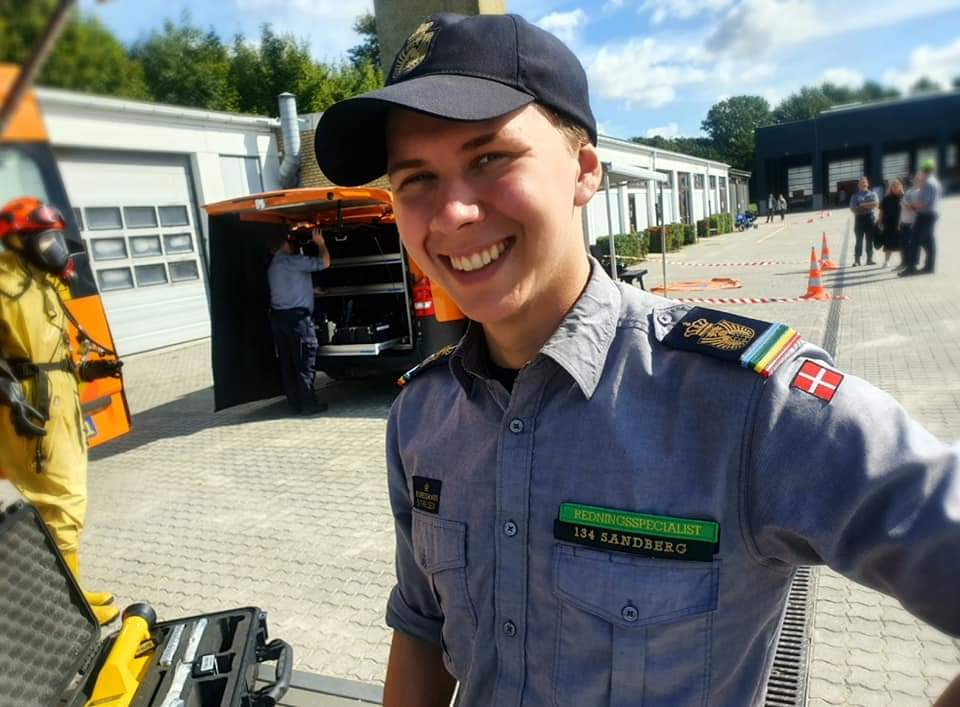
\includegraphics[width=0.5\linewidth]{BRSS.jpg}
    \caption{Åben Hus Beredskabsstyrelsen Sjælland}
\end{figure}
\newpage \section{Gode Råd}
\begin{minipage}[t]{0.5\textwidth}
\textbf{Ingredienser:}
\begin{itemize}
    \item 3 æg
    \item 100 g sukker
    \item 250 g hvedemel
    \item 1.5 tsk kardemomme 
    \item 125 g smeltet margarine
    \item 1/2 dL mælk
\end{itemize}
\end{minipage}
\begin{minipage}[t]{0.5\textwidth}
\textbf{Fremgangsmåde:}
Havde lidt problemer med at tyde opskriften i tide, så derfor kommer der bare et billede af farmos opskrift i på følgnende side.
\end{minipage}
\newpage \begin{figure}[h]
    \centering
    \includegraphics[width=0.5\linewidth]{Billeder//Dessert/Gode råd.jpg}
    \caption{Farmors opskrift på gode råd}
\end{figure}
\newpage \section{Ris a la Mande}
\begin{minipage}[t]{0.5\textwidth}
\textbf{Ingredienser:}
\begin{itemize}
    \item 1L sød mælk
    \item 75 g sukker
    \item 1 stk vaniljestang, flækket (skåret over langs midten)
    \item 180 g grødris
    \item 100 g mandler, hakkede og smuttede
    \item 1 knivspids salt
    \item 4 dL piskefløde
\end{itemize}
\end{minipage}
\begin{minipage}[t]{0.5\textwidth}
\begin{enumerate}
    \item Bring sødmælk i kog under opsyn (rør i den en gang imellem).
    \item Skru ned for varmen når sødmælken begynder at dampe, og ad stå under låg i 2 minutter.
    \item Vend den flækket vaniljestang i sukker således vaniljekornene inden i ikke klumper, og smid det hele (inklusiv den hele stang), i mælken. 
\item Kog i 20 minutter, og lad køle af, tilsæt de hakkede smuttede mandler.
\item Pisk fløden til flødeskum og vend i risengrøden, omtrent 1 time inden servering.
\end{enumerate}
\end{minipage}
\newpage \begin{tikzpicture}[remember picture,overlay,inner sep=0pt,outer sep=0pt]
    \node[anchor=south east] at (current page.south east) {
        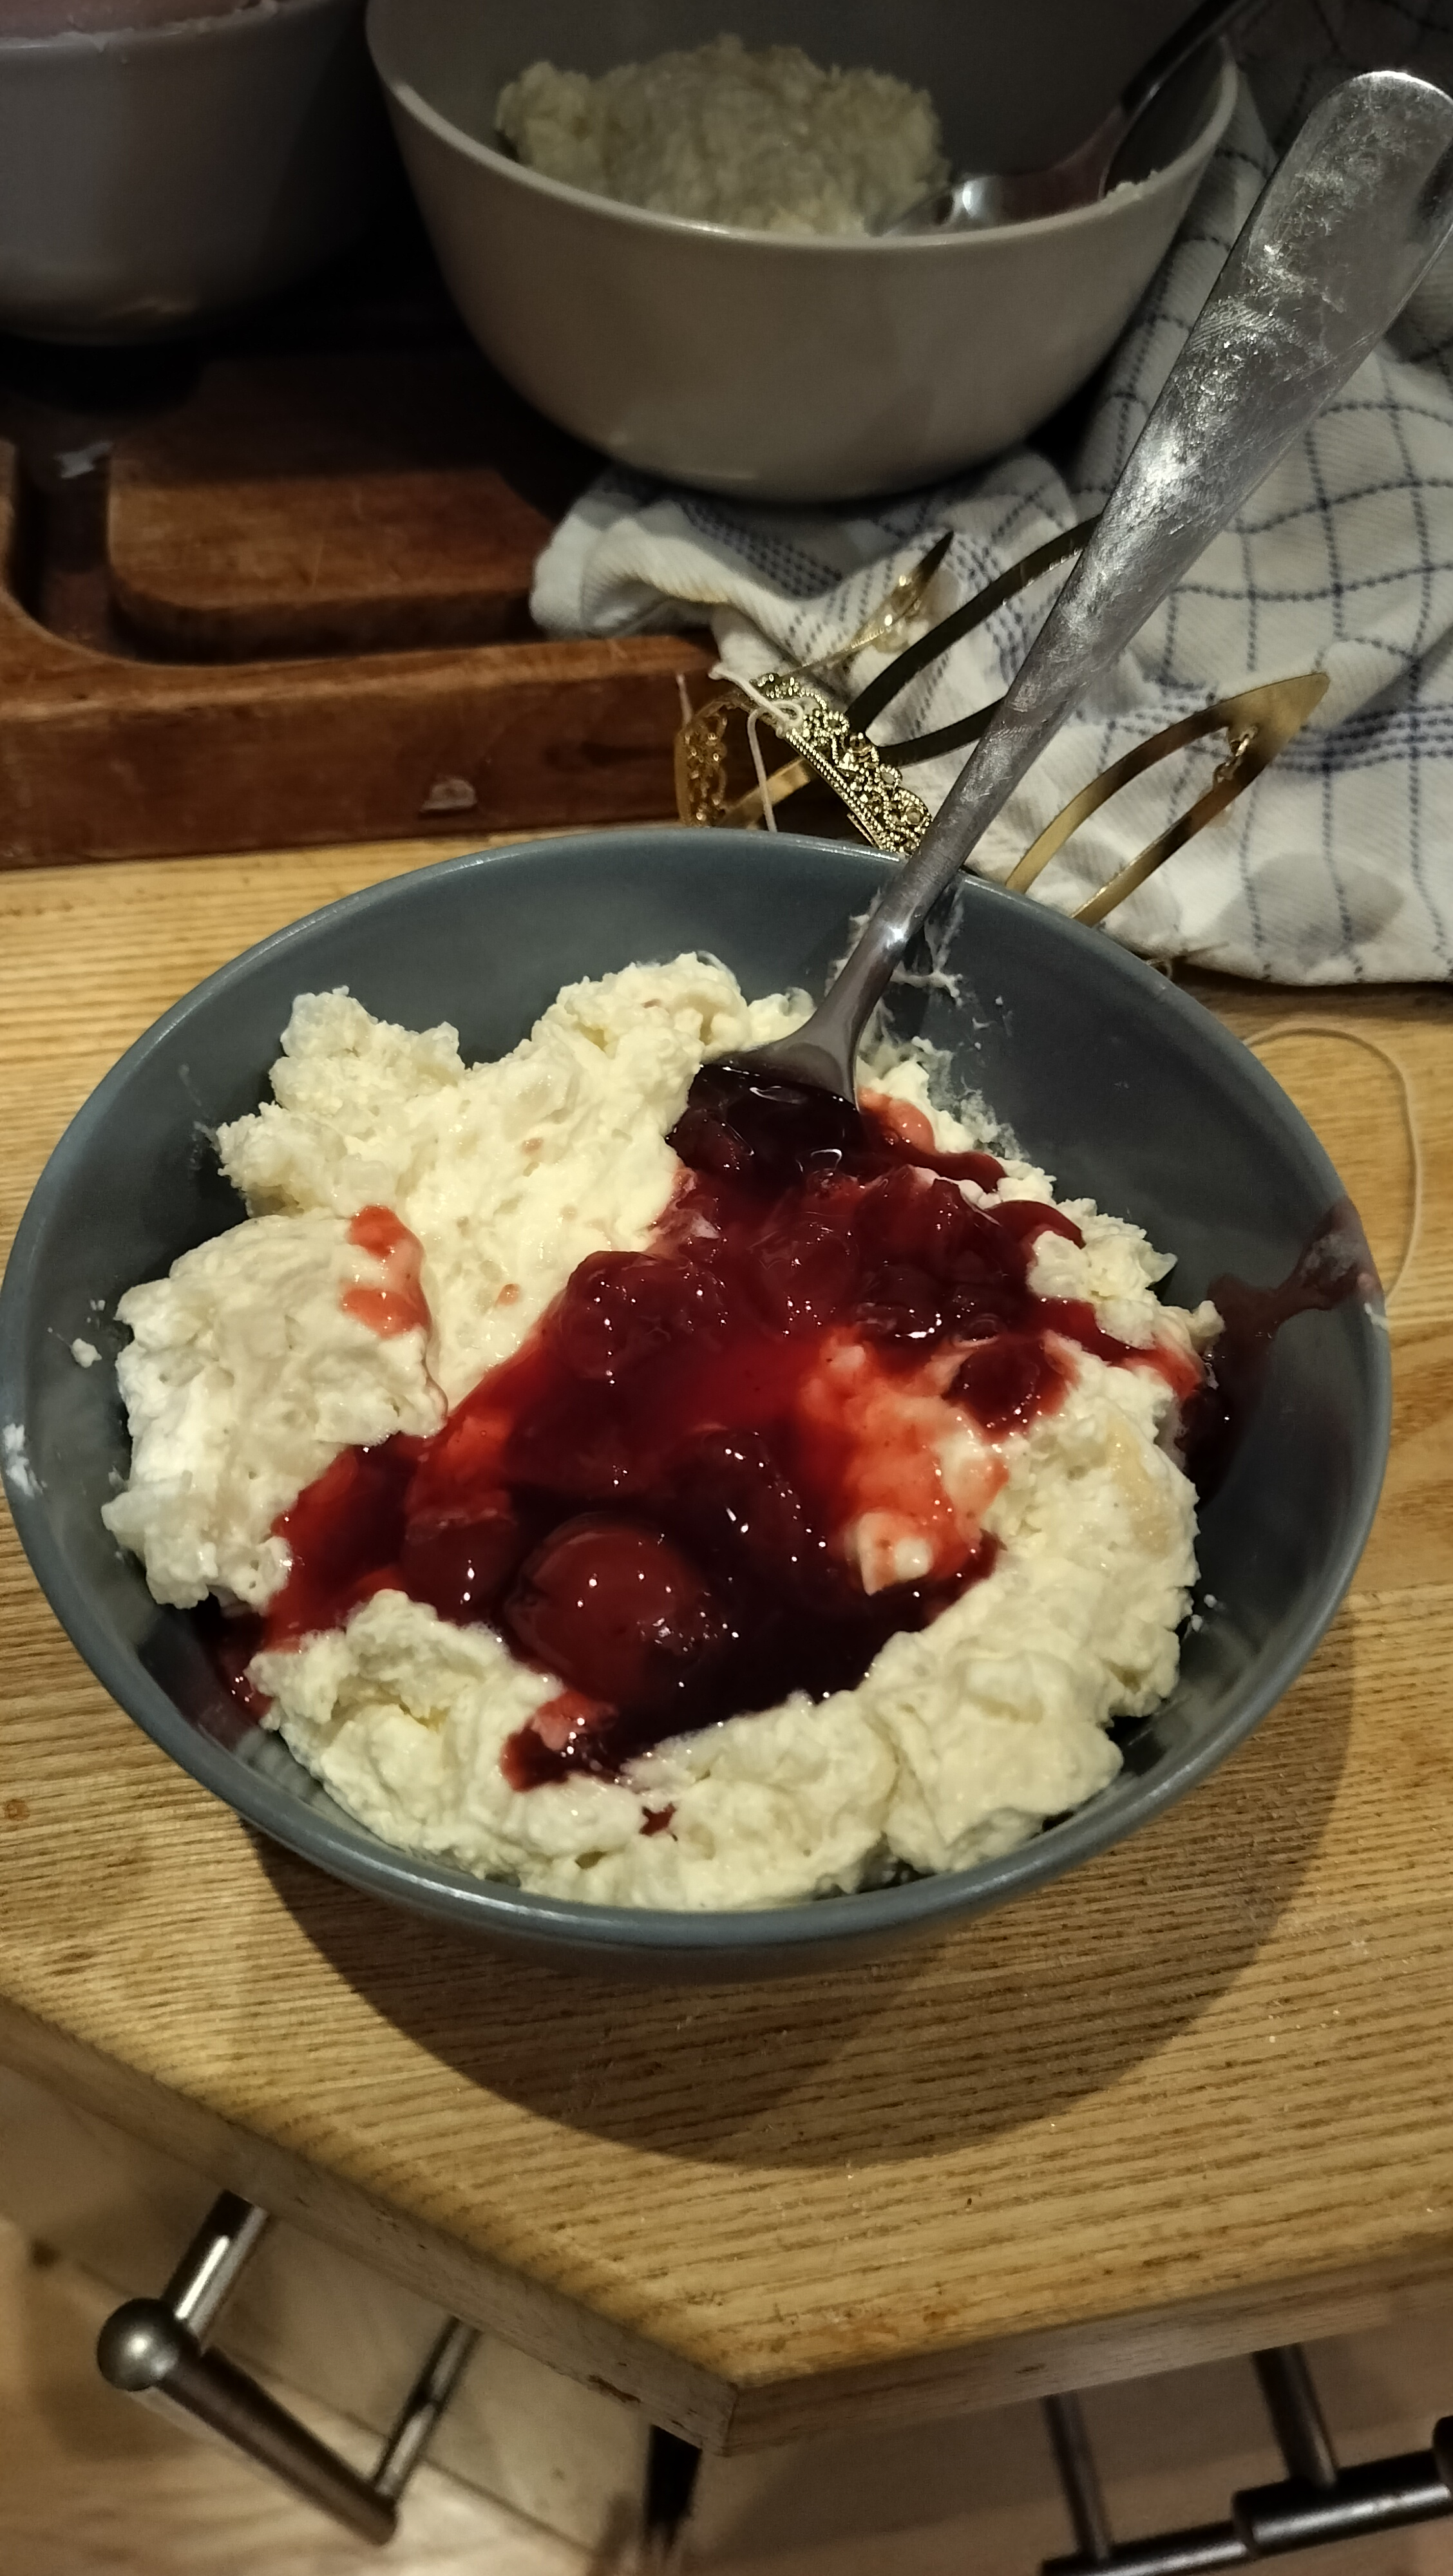
\includegraphics[width=\paperwidth,height=\paperheight]{Billeder/Dessert/Ris_a_La_mande.jpg}
    };
\end{tikzpicture}
\newpage \section{Marengs}
\begin{minipage}[t]{0.5\textwidth}
\textbf{Ingredienser:}
\begin{itemize}
    \item 140 g æggehvider
    \item $\sim$ 300 g flormelis
\end{itemize}
\end{minipage}
\begin{minipage}[t]{0.5\textwidth}
\textbf{Fremgangsmåde:}
\begin{enumerate}
    \item Forvarm ovn til 80 \degree C
    \item Pisk æggehviden til de ikke længere er gennemsigtige
    \item Tilføj dernæst flormelissen lidt efter lidt
    \begin{itemize}
        \item At tilføje flormelis til æggehviden minder meget om når man laver glasur, tilsæt de lidt efter lidt til det til sidst er "svært" at opløse mere flormelis i
    \end{itemize}
    \item Pisk mere end man umiddelbart skulle tro, det skal blive meget luftigt
    \item Put ned i pose, til at trykke ud som "kys". Eller hæld i springform til brug til kage
    \item Bag i ovnen ved 80 \degree C i \~ \space 1 time
\end{enumerate}
\end{minipage}
\textcolor{white}{white}\\
Til sidst kan der eventuelt skrues op for varmen, men dette giver "pludselig" udvidelse af marengsene, men sikre de bliver færdige.
OBS. Prøv at lave dem så tynde/luftige som muligt da de ellers kan blive klistrede indeni. De skal dermed have længere i ovnen, for at bliver bagt helt igennem, og dermed forårsage at de bliver lidt gyldne/ en smule brændte på ydersiden.  
\newpage \begin{tikzpicture}[remember picture,overlay,inner sep=0pt,outer sep=0pt]
    \node[anchor=south east] at (current page.south east) {
        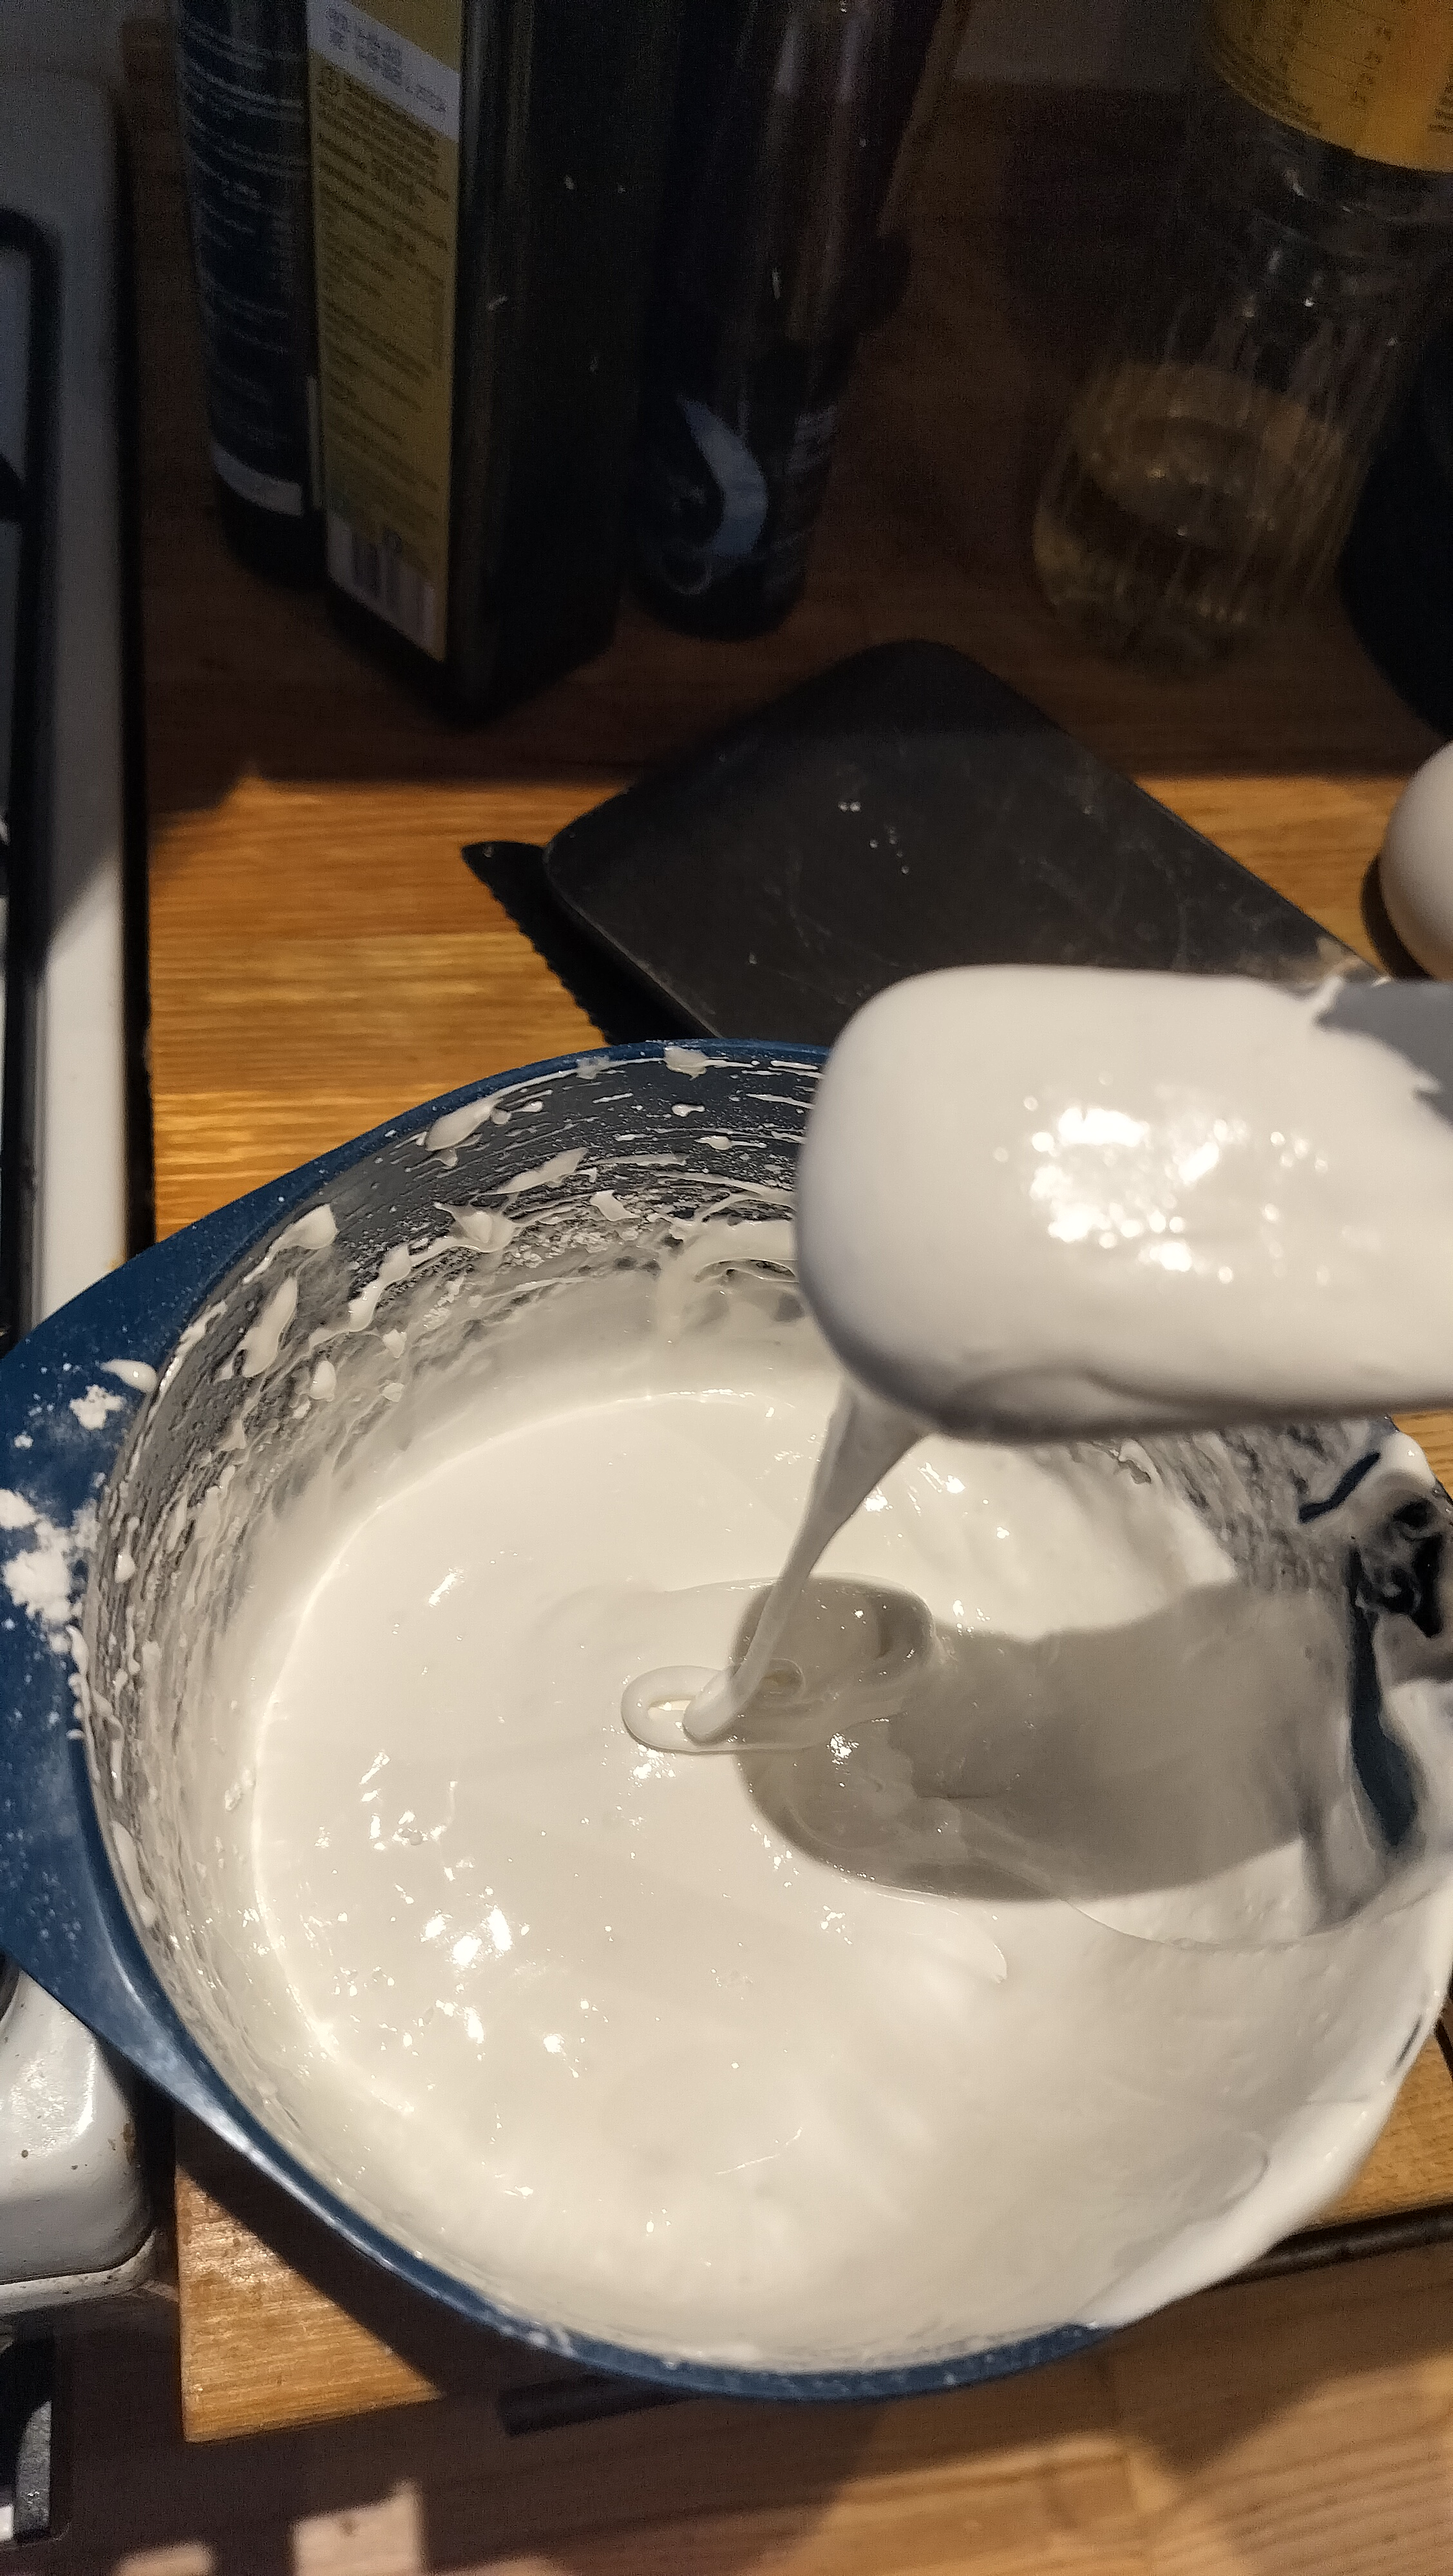
\includegraphics[width=\paperwidth,height=\paperheight]{Billeder/Dessert/Marengs_Flydende.jpg}
    };
\end{tikzpicture}
\chapter{Brød}
\minitoc
Synes især at jeg har haft stor succes i forhold til bagning af brød. Har som udgangspunkt ikke talt det med som en ny af de månedlige opskrifter. Har desværre ikke været så god til at huske at tage billeder af brødet, så lige nu kommer det bare til at være arbitrære billeder. Har dog heldigvis fået indhentet nogle på det sidste.
\newpage \section{Brioche}
\begin{minipage}[t]{0.5\textwidth}
\textbf{Ingredienser:}
\begin{itemize}
    \item 3 dL mælk
    \item 25 g gær
    \item 2 æg
    \item 125 g smør, skåret i tern, stuetempereret
    \item 2 spsk sukker
    \item 1.5 tsk salt
    \item 1 knivspids stødt kardemomme
    \item 550 g hvedemel
\end{itemize}
Pensling:
\begin{itemize}
    \item 1 æg
    \item Evt. sesamfrø
    \item Evt. græskarkerne
\end{itemize}
\end{minipage}
\begin{minipage}[t]{0.5\textwidth}
\textbf{Fremgangsmåde:}
\begin{enumerate}
    \item Varm mælken til lunken, og rør gæren ud i.
    \item Tilsæt æg, smør, sukker, salt, kardemomme og 250g af hvedemelet.
    \item Rør dejen sammen til ensartet konsistens, tilsæt dejen lidt efter lidt.
    \item Lad dejen hæve i 2 timer ved stuetemperatur.
    \item Form dejen til boller (cirka 10), og lad dem stå til hævning i en time.
    \item Pensel med æg og tilsæt ønskede krydderier, og bag i forvarmet ovn på 175 \degree C varmluft i omtrent 20 minutter
\end{enumerate}
\end{minipage}
\newpage Her kunne der være et billede af nogle briocheboller, men i stedet for er der et billede af Artemis
\begin{figure}
    \centering
    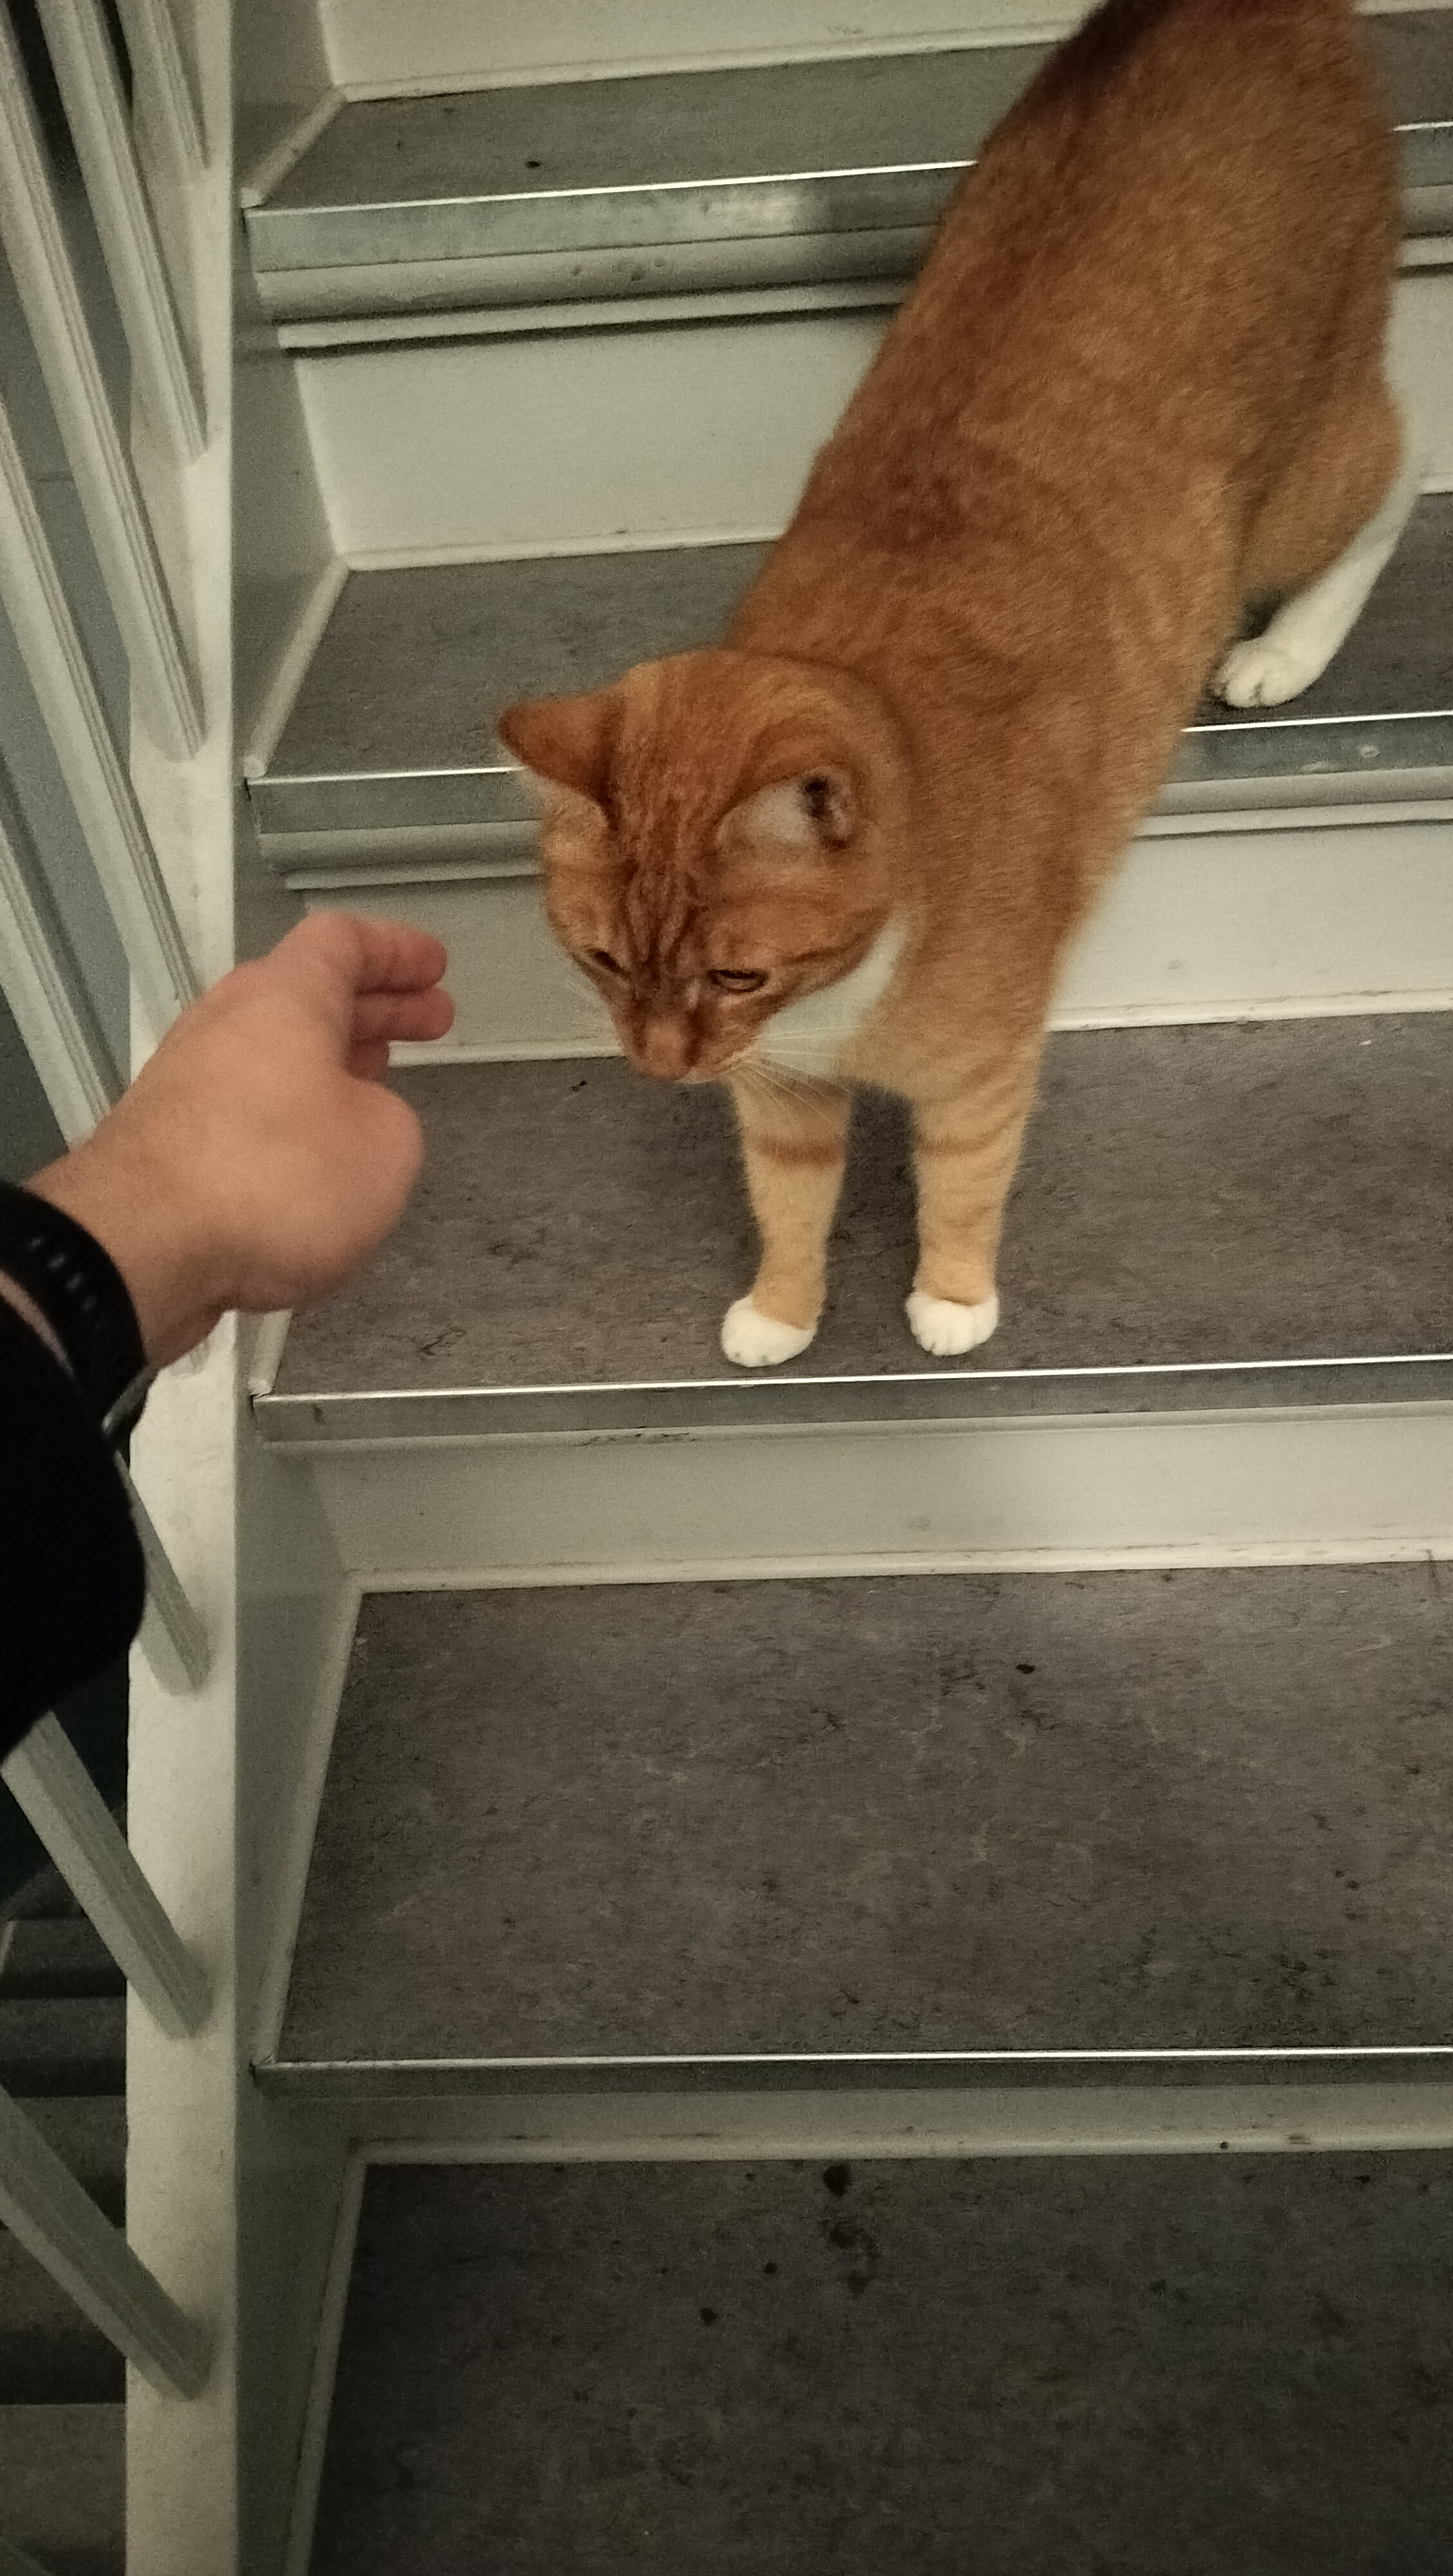
\includegraphics[width=0.5\linewidth]{IMG20231108195607.jpg}
    \caption{Artemis}
\end{figure}
\newpage \section{Ciabattabrød}
\begin{minipage}[t]{0.5\textwidth}
\textbf{Ingredienser:}
\begin{itemize}
    \item 7 dL lunkent vand (stuetemperatur)
    \item 10 g gær
    \item 2 tsk sukker
    \item 2 tsk salt
    \item 800 Manitoba hvedemel
\end{itemize}
Pensling
\begin{itemize}
    \item 2 spsk olivenolie
    \item Evt. Timian
    \item Flagesalt eller groft salt
\end{itemize}
\end{minipage}
\begin{minipage}[t]{0.5\textwidth}
\textbf{Fremgangsmåde:}
\begin{enumerate}
    \item Hæld vandet i en skål, og rør sukker og gær ud.
    \item Tilsæt melet og saltet til vandet.
    \item Rør dejen til en ensartet masse, dæk til med viskestykke og lad hæve i 5 timer.
    \item Hæld dejen ud på et meldækket bord, og fold dejen gentagne gange.
    \item Del dejen i 2 stykker, pensel med olivenolie, og læg på en bageplade.
    \item Bag i en forvarmet ovn på 275 \degree C varmluft.
\end{enumerate}
\end{minipage}
\newpage \begin{tikzpicture}[remember picture,overlay,inner sep=0pt,outer sep=0pt]
    \node[anchor=south east] at (current page.south east) {
        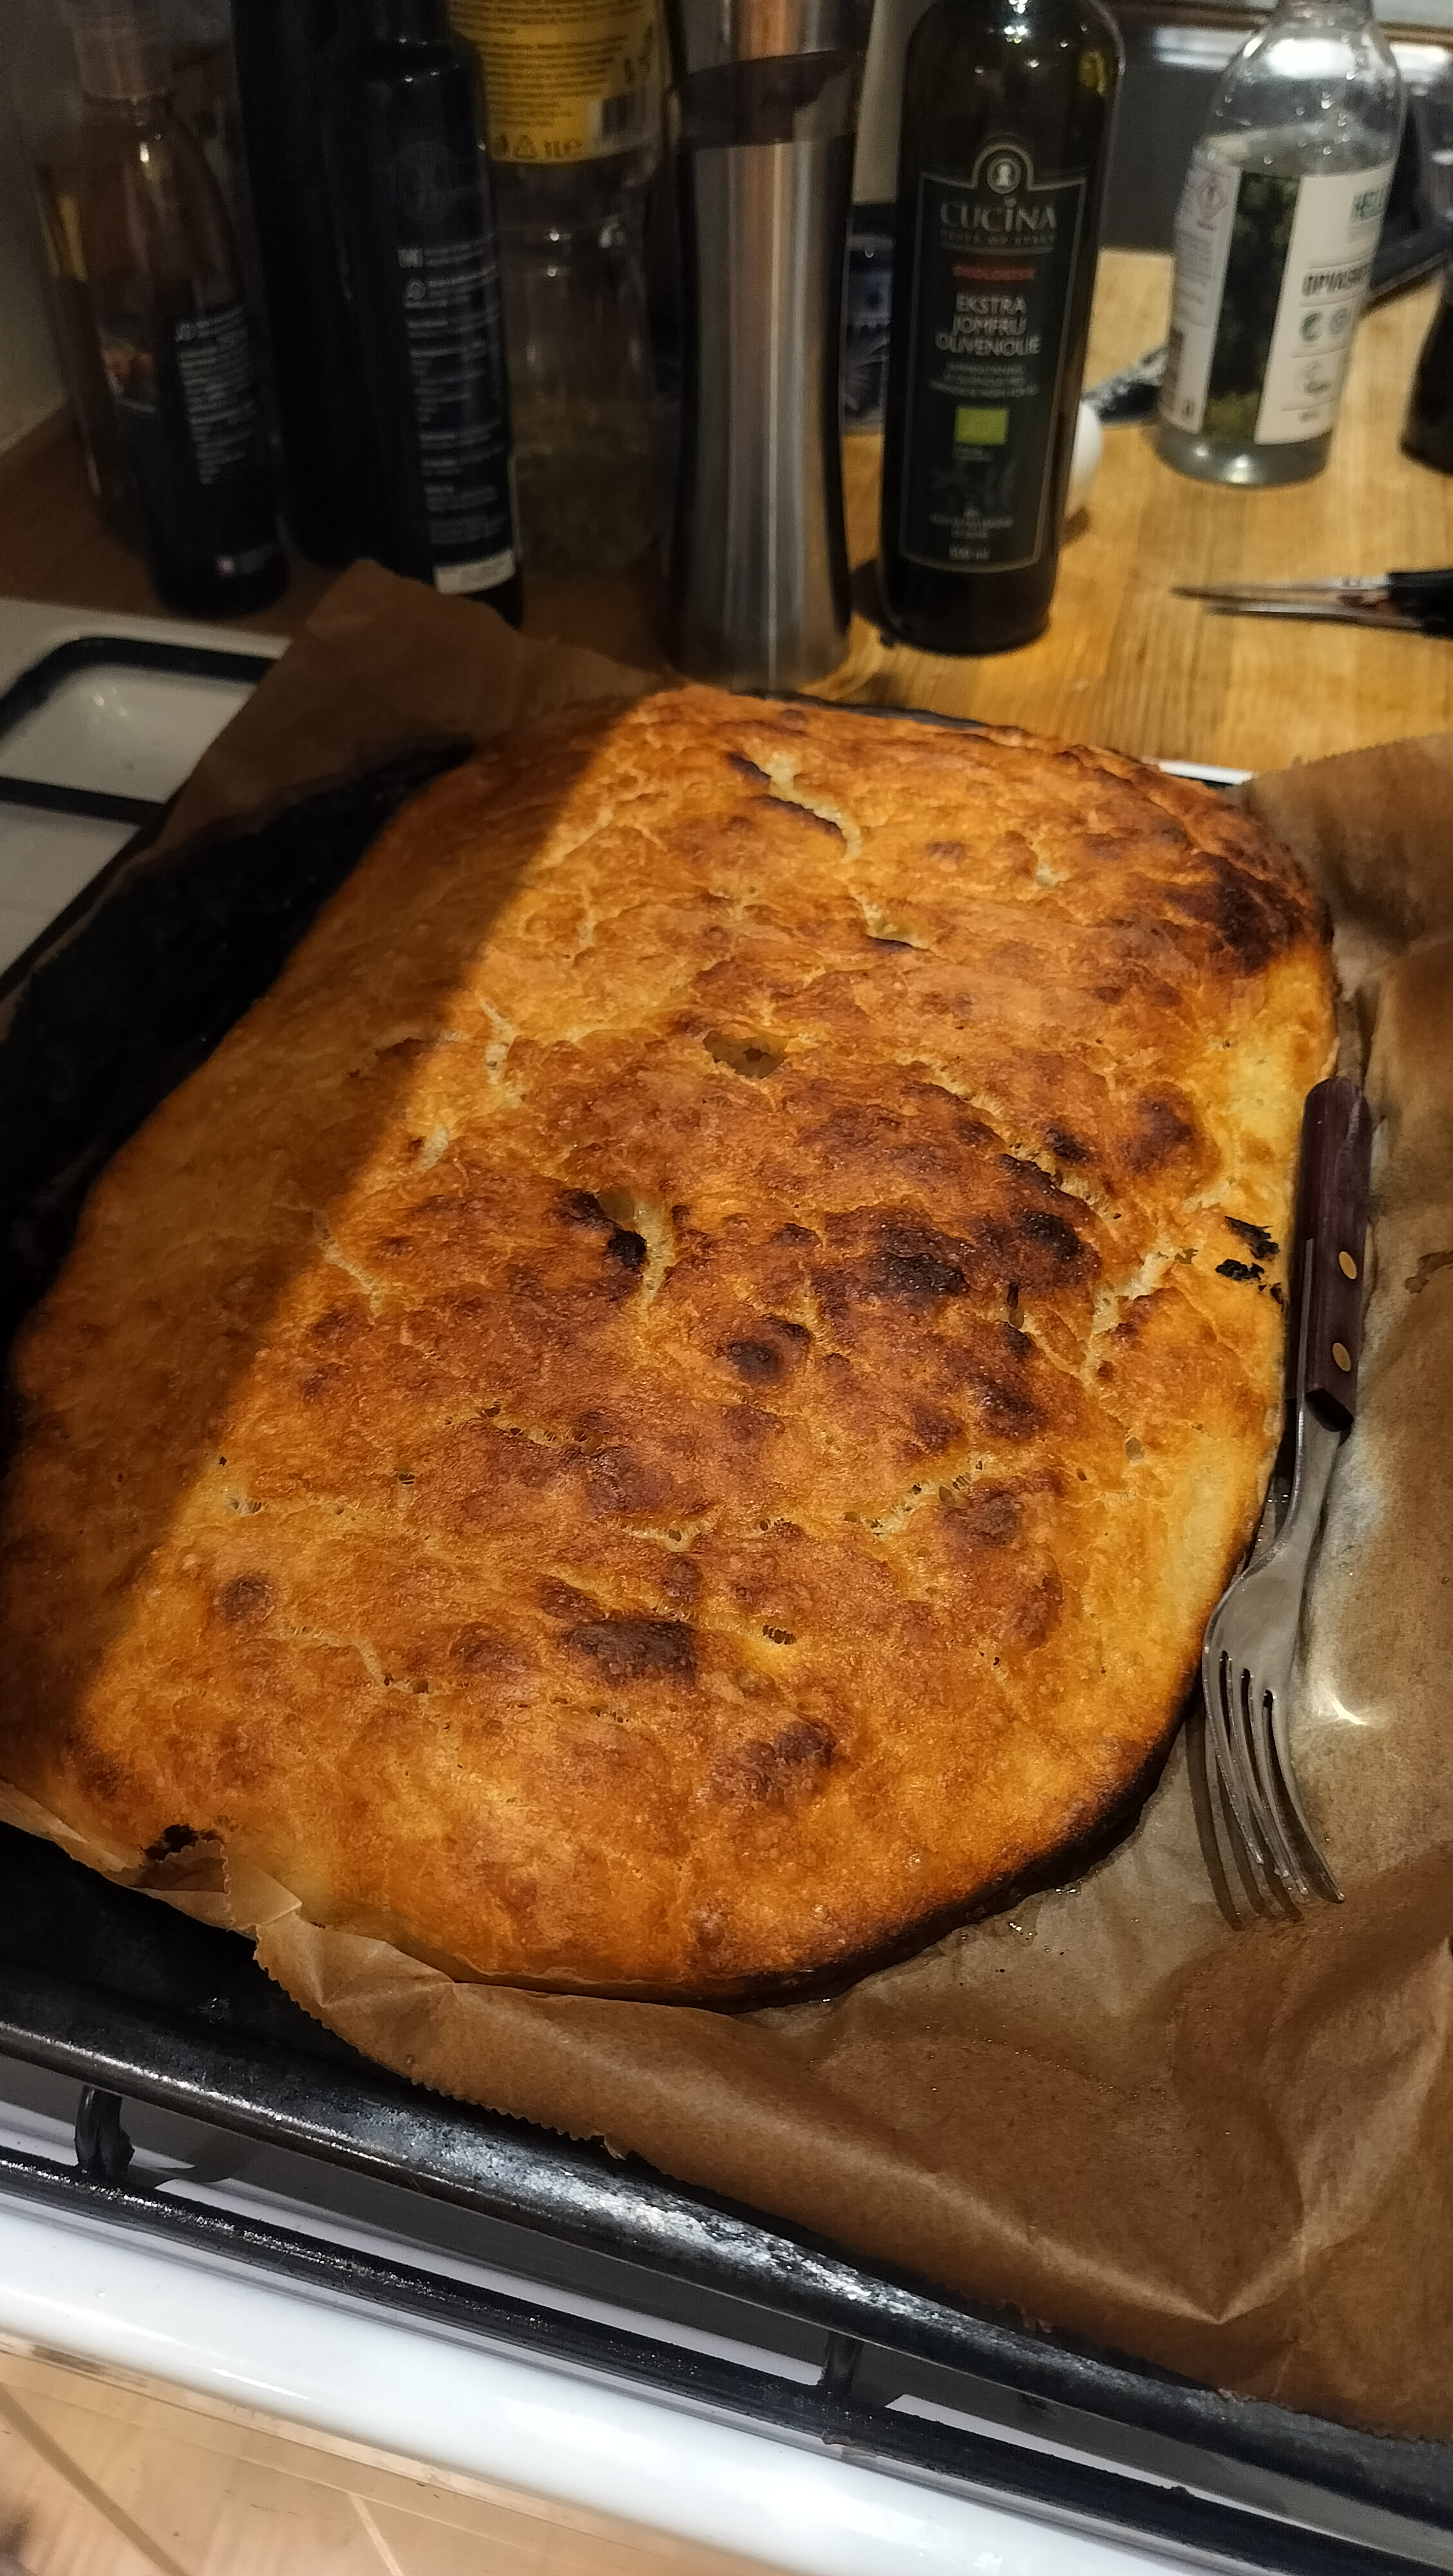
\includegraphics[width=\paperwidth,height=\paperheight]{Billeder/Brød/Ciabatta.jpg}
    };
\end{tikzpicture}
%\newpage Her skulle der også været et billede, så i stedet for kommer der et billede af Devils Starways
%\begin{figure}
%    \centering
%    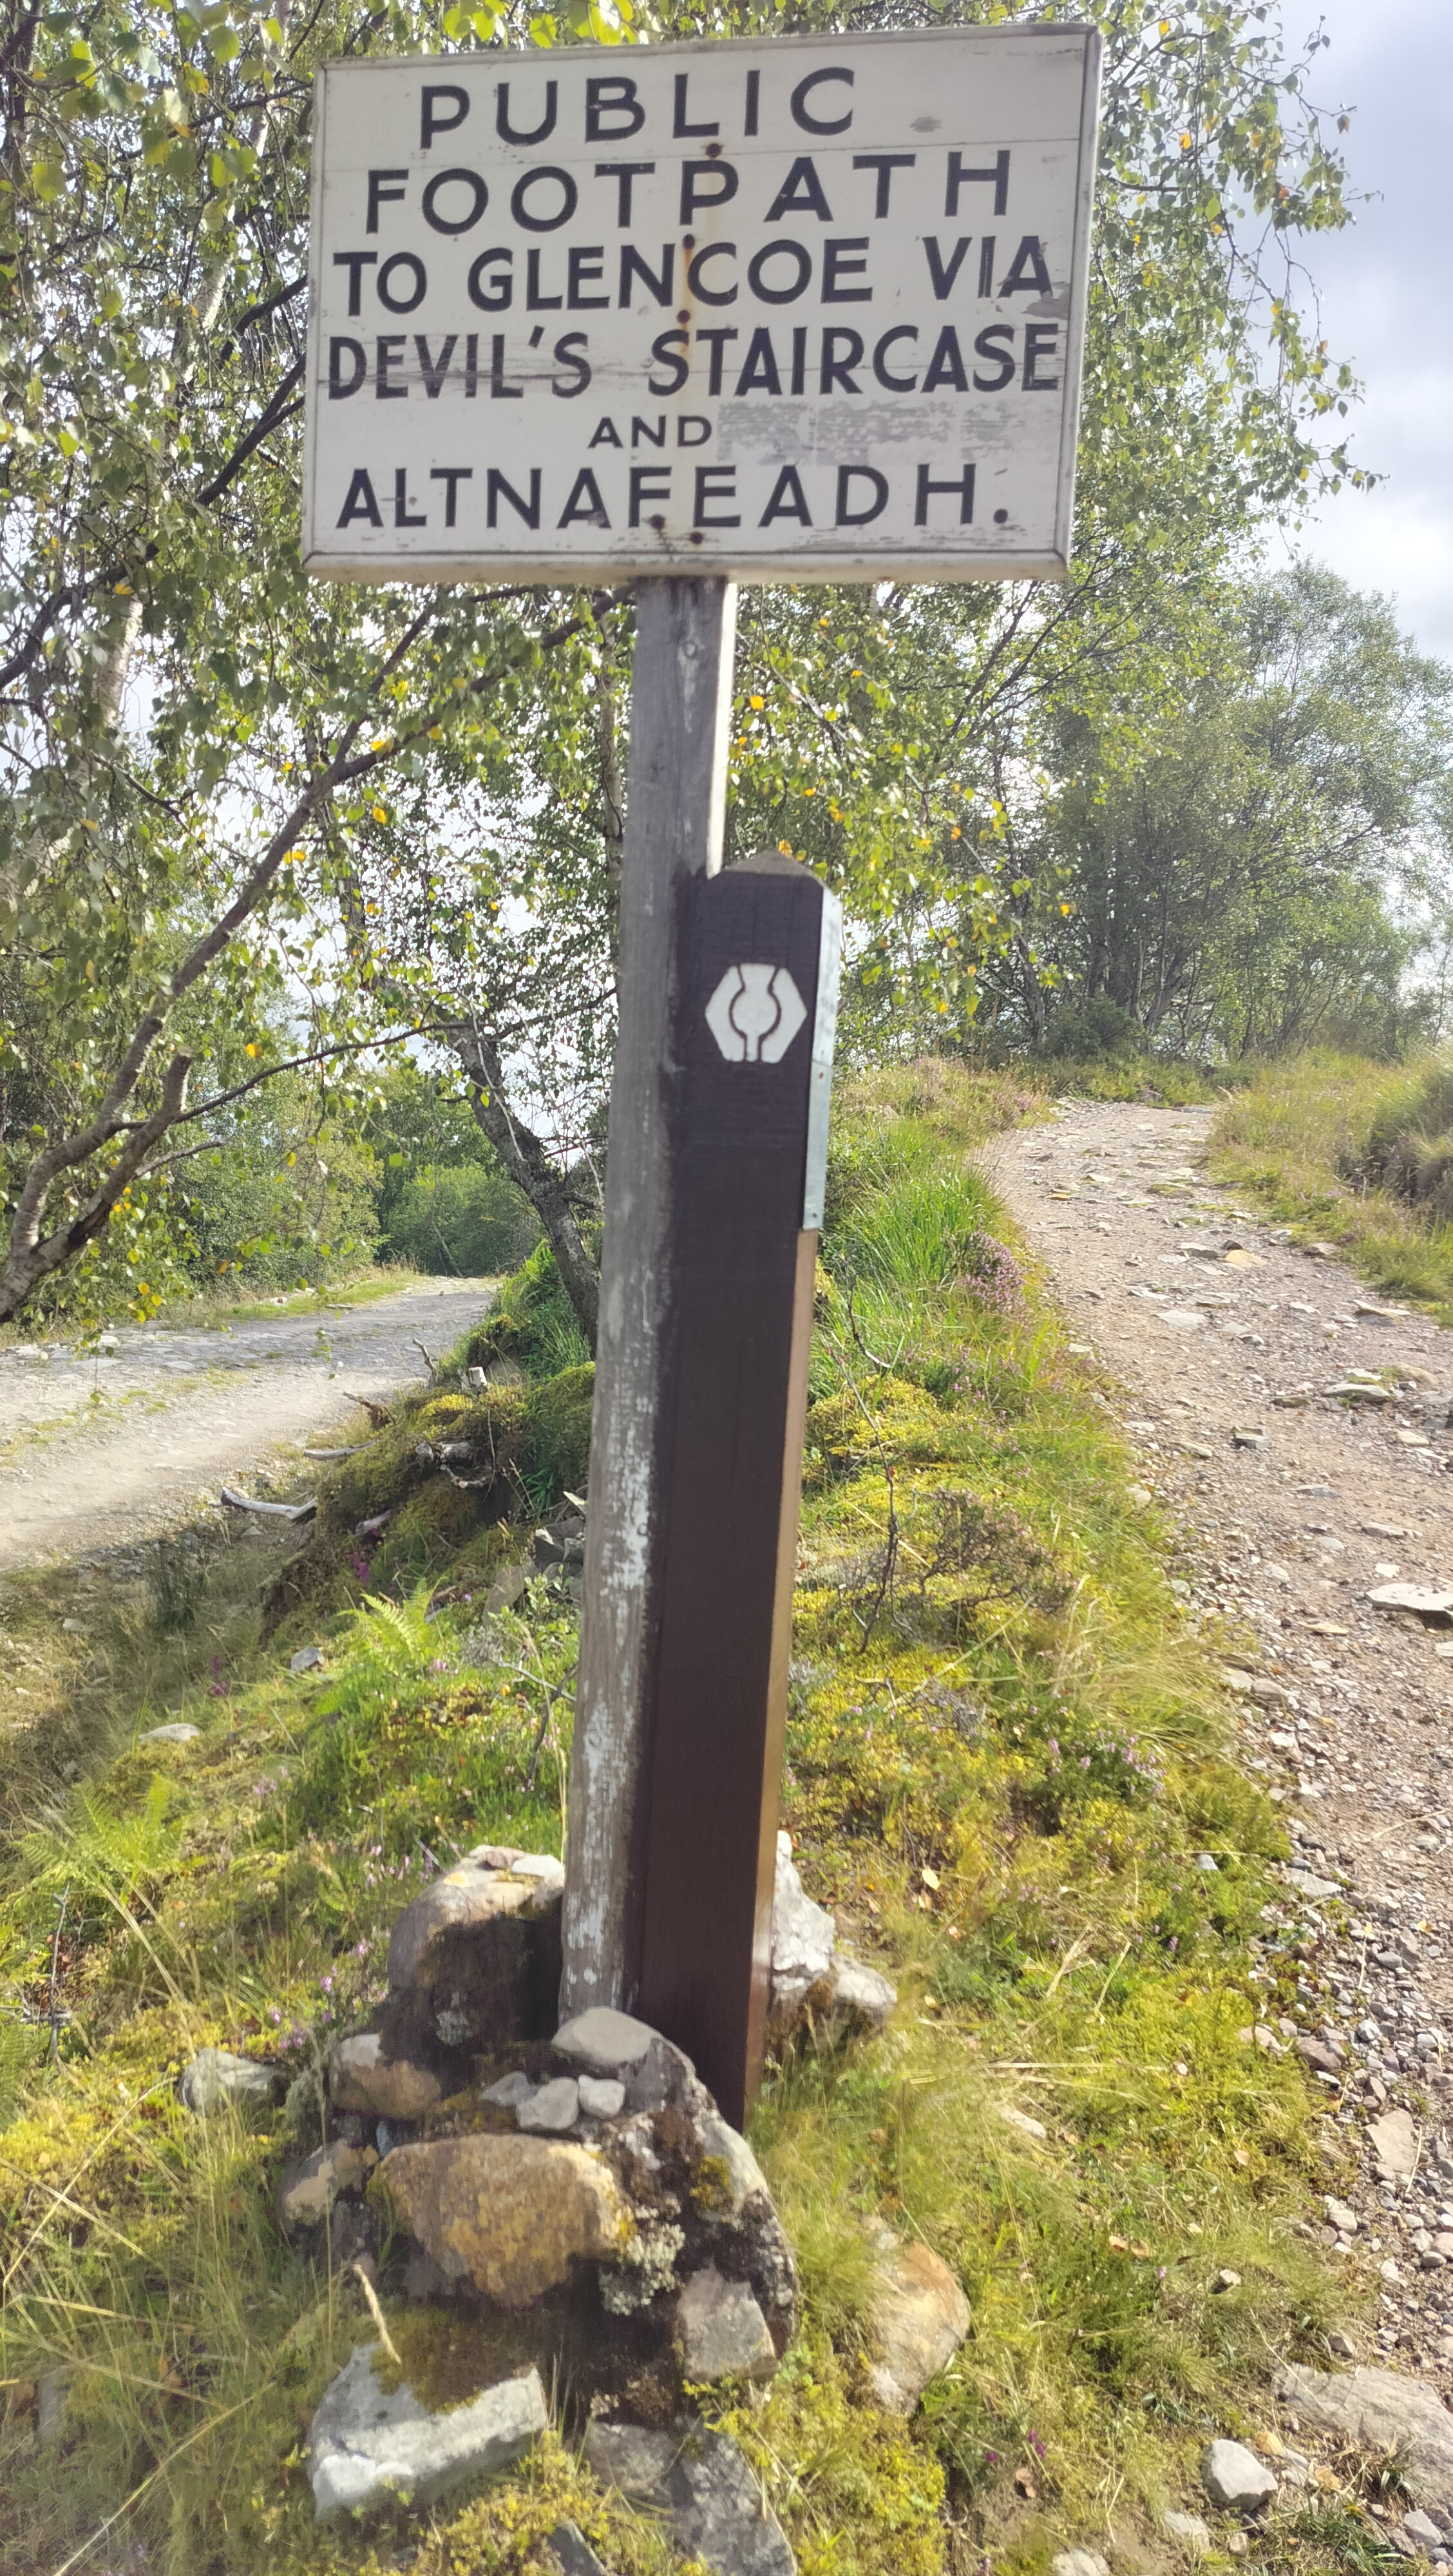
\includegraphics[width=0.5\linewidth]{Devils_stairway.jpg}
%    \caption{Devils stairway}
%\end{figure}
\newpage \section{Focaccia}
\begin{minipage}[t]{0.5\textwidth}
\textbf{Ingredienser:}
\begin{itemize}
    \item 4 dL vand
    \item 20 g gær
    \item 3 spsk olivenolie
    \item 1 tsk salt
    \item 100 g grahamsmel
    \item 400 g hvedemel
\end{itemize}
Topping:
\begin{itemize}
    \item 1 tsk flagesalt (eller groft salt)
    \item 4 fed hvidløg, presset
    \item Rosmarin (eventuelt frisk)
    \item Evt. 100 g oliven, skiveskåret
    
\end{itemize}
\end{minipage}
\begin{minipage}[t]{0.5\textwidth}
\textbf{Fremgangsmåde:}
\begin{enumerate}
    \item Rør gæren ud i en skål med vand.
    \item Tilsæt olien, saltet og grahamsmellen og rør rundt.
    \item Tilsæt hvedemelet lidt efter lidt, og ælt til dejen er klistret og blød.
    \item Dæk dejen til og lad den hæve i 1 time.
    \item Læg dejen ud på en bradepande, og lad den hæve en halv time yderligere.
    \item Tryk fordybninger i dejen, og pensel med olivenolie og drys de ønskede toppings.
    \item Bag i en forvarmet ovn ved 180 \degree C i 20 minutter
\end{enumerate}
\end{minipage}
\\ Når man lader dejen hæve på en bradepande er det vigtigt det ikke er for lang tid, en længerevarende hævning får brødet til at "miste" pusten, dette giver en mindre hævning under bagning og i sidste ende et mindre luftigt brød. 
Focaccia er et relativ hurtigt brød at bage med en vente tid på omtrent 1 time og 50 minutter med 10-15 minutters arbejdstid. En samlet tid på \underline{2 timer og 5 minutter}
\newpage \begin{tikzpicture}[remember picture,overlay,inner sep=0pt,outer sep=0pt]
    \node[anchor=south east] at (current page.south east) {
        \includegraphics[width=\paperwidth,height=\paperheight]{Billeder/Brød/Focaccia.jpg}
    };
\end{tikzpicture}
\newpage \section{Naan}
\begin{minipage}[t]{0.5\textwidth}
\textbf{Ingredienser:}
\begin{itemize}
    \item 1 dL stuetempereret vand
    \item 25 g gær
    \item 1 dL mælk
    \item 1 æg, sammenpisket
    \item 1 dL græsk yoghurt 10\%
    \item 3 spsk olivenolie
    \item1 tsk salt
    \item1 tsk sukker
    \item450 g hvedemel
\end{itemize}
    Pensling og smag
\begin{itemize}
    \item 50 g smør, smeltet
    \item Friske koriander, finthakket
    \item 2 fed hvidløg, pressede
    \begin{itemize}
        \item  evt 1 spsk nigella frø. \\
        Nigella frø kan fås i Inco og lignende (jeg synes ikke de tilføje det store til smagen, men giver noget til looket)
        \end{itemize}
\end{itemize}
\end{minipage}
\begin{minipage}[t]{0.5\textwidth}
\begin{enumerate}
    \item Kom vand i en skål og rør gær ud i væsken. Tilsæt mælk, æg, yoghurt, olivenolie, sukker og salt samt 250g af  melet. 
    \item Rør det grundigt igennem og tilsæt så lidt efter lidt mere mel.Ælt dejen godt, til den er smidig, blød og stadig klistret og kom den i en skål.
    \item Dæk dejen til og lad den hæve i en times tid til omtrent dobbelt størrelse. Del dejen i 2 dele og tryk eller rul hver del flad og i dråbeform. 
    \item Læg dem på en bageplade med bagepapir, dæk dem til og lad dem hæve i et kvarters tid.
    \item Pensl brødene med smeltet smør og drys med de ønskede krydderier.
    \item Bag brødene i en forvarmet ovn ved 175 \degree C varmluft i cirka 20 minutter.

\end{enumerate}
\end{minipage}

\newpage \begin{tikzpicture}[remember picture,overlay,inner sep=0pt,outer sep=0pt]
    \node[anchor=south east] at (current page.south east) {
        \includegraphics[width=\paperwidth,height=\paperheight]{Billeder/Brød/Naan.jpg}
    };
\end{tikzpicture}
\newpage \section{Pizzadej}
\begin{minipage}[t]{0.5\textwidth}
\textbf{Ingredienser:}
\begin{itemize}
    \item 25 g gær eller 5 g gær til koldhævning
    \item 2.5 dL vand
    \item 3 spsk olivenolie
    \item 1 tsk salt
    \item 500g hvedemel
\end{itemize}
\underline{Ekstra:}
    \begin{itemize}
        \item  1 spsk olivenolie til smøring
        \item Masser af mel til udrulning
    \end{itemize}
\end{minipage}
\begin{minipage}[t]{0.5\textwidth}
\textbf{Fremgangsmåde:}
\begin{enumerate}
    \item Bland gæren med lunkent vand, 25 gram til ~1 times hævning og 5g til koldhævning
    \item Kom 1/3 af melen i, olivenolien og salt i og rør til ens konsistens, dernæst tilføj det sidste mel lidt efter lidt
    \item Drys mel på bordet og ælt dejen til smidig. Olier en skål og kom dejen i, tildæk med viskestykke og lad hæve i 1 time eller natten over
    \item Til sidst kan dejen med fordell deles i 2, så der kan laves med 2 forskellige slags fyld, bag i 250 \degree C forvarmet ovn i cirka 10 minutter 
\end{enumerate}
\end{minipage}
\newpage 
Her mangler der igen et billede så der kommer et billede af et meget stort spidskål 
\begin{figure}
    \centering
    \includegraphics[width=0.5\linewidth]{Spidskål.jpg}
    \caption{Spidskål}
\end{figure}

% \chapter{Drinks}

\end{document}
